\documentclass[a4paper,oneside,11pt]{book}
	
\usepackage[spanish]{babel}
\usepackage[utf8]{inputenc}

% -------------------------------------------------------------------------
% puede que queramos usar el símbolo del euro.
\usepackage{eurosym}
% Para incluir graficos en JPG => compilar con pdflatex.
%\usepackage[pdftex]{graphicx}
% Para incluir graficos EPS => compilar con latex.
\usepackage[dvips]{graphicx}
% Para escribir en color cuando compilamos con pdflatex
\usepackage[pdftex,usenames,dvipsnames]{color}
\definecolor{gray}{RGB}{235,235,235}

\usepackage{float} % para incluir [H] (here) en las imágenes
% -------------------------------------------------------------------------
\usepackage{hyperref} % Para incluir enlaces
% -------------------------------------------------------------------------

% Paquete fancyhdr -> Para modificar la cabecera y pie de paginas.
% http://tug.ctan.org/tex-archive/macros/latex/contrib/fancyhdr/
\usepackage{fancyhdr}
\usepackage{fancybox}
\pagestyle{fancy}
\fancyhf{}
\fancyhf[HR]{\thepage}
\fancyhf[HL]{\nouppercase\rightmark}
\headwidth=16cm

% Para incluir subfiguras.
\usepackage{subfigure}

% Ajuste de margenes
\usepackage{anysize}
\marginsize{3cm}{2cm}{2cm}{2cm}	% izquierda, derecha, arriba, abajo
\parskip=6pt	% Personalizamos la separacion entre parrafos.
\parindent=10pt	% Personalizamos el identado en la primera linea del nuevo parrafo.
\setcounter{secnumdepth}{3}	% Numero maximo de niveles de profundidad en las secciones.

% -------------------------------------------------------------------------

% Package booktabs -> Para mejorar el aspecto de las tablas o cuadros.
% http://www.ctan.org/tex-archive/macros/latex/contrib/booktabs/
\usepackage{booktabs}

% Package rotating -> Para poder girar las tablas y dibujarlas a lo largo
% del folio en vez de a lo ancho.
\usepackage{rotating}

% Packages multicol y multirow, para manejar tablas de filas y columnas multiples.
\usepackage{multicol}
\usepackage{multirow}

\usepackage{tabularx}


% Packages para apendices y renombrado de la pagina de apendices
\usepackage{appendix}
\renewcommand{\appendixname}{Apéndices}
\renewcommand{\appendixtocname}{Apéndices}
\renewcommand{\appendixpagename}{Apéndices}
% -------------------------------------------------------------------------
% Compilar con bibtex book.gls.aux
\usepackage[refpages]{gloss}
% -------------------------------------------------------------------------
\usepackage[margin=2cm,font=footnotesize,labelfont=bf]{caption} 
% -------------------------------------------------------------------------
% Comando para realizar las referenfias a etiquetas
\newcommand{\fullref}[1]{\ref{#1} de la página \pageref{#1}}
% -------------------------------------------------------------------------

\title{\bf Desarrollo Aplicación Web de Gestión Deportiva para Entrenadores de Natación}
\author{Roberto Marco Sánchez}
\date{\today}

\begin{document}
	
	% \maketitle sirve para generar automática una portada predefinida. Se incluye portada personalizada
	\include{pfc_portada}

	% Documentos adicionales
	%
% Certificado
%

\begin{center}
	\begin{minipage}[t][6cm][l]{.8\textwidth}
		\begin{center}
			% Nombre del director del proyecto
			D. {\sc Borja Rubio reyes}

			% A los profesores les gusta que se indique su grado o posición en la estructura de la universidad :-P
			Profesor de Escuela Ingeniería Informática

			% Departamento al que pertenece el director y en el que se realiza el proyecto.
			Departamento de Ingeniería del Software

			Universidad de Las Palmas de Gran Canaria
		\end{center}
	\end{minipage}
\end{center}

% El director certifica que el proyecto obra de su proyectando constituye su Proyecto de Fin de Carrera en la titulación indicada.
CERTIFICA:
Que la memoria titulada {\it ``Aplicación Web de Gestión Deportiva para Entrenadores de Natación''} ha sido realizada por {\sc Roberto Manuel Marco} bajo mi dirección y constituye su Proyecto de Fin de Carrera de Ingeniería Informática.

\vspace{5cm}

En Las Palmas de Gran Canaria, a \today

% Espacio para que pueda firmar el certificado que debe acompañar al proyecto.
\vspace{3cm}

\begin{center}
	\begin{minipage}[t][4cm][l]{.5\textwidth}
	% Nombre del director del proyecto
	D. {\sc Borja Rubio Reyes}
	\\
	Tutor del proyecto
	\end{minipage}
\end{center}

	%
% Resumen del proyecto de fin de carrera
%

\section*{Resumen:}

Lorem ipsum dolor sit amet, consectetuer adipiscing elit. Nullam at lacus quis massa condimentum faucibus. In facilisis augue sit amet mi. Nulla hendrerit aliquam nunc. Vestibulum sed elit. Sed tempus porttitor lorem. Nulla facilisi. Vestibulum a sem ut ligula molestie tempor. Sed lacinia ultricies neque. Integer vitae lacus. Vestibulum ante ipsum primis in faucibus orci luctus et ultrices posuere cubilia Curae; Nullam rutrum lacus at nisi. Integer ultrices velit et diam. Phasellus sed justo eu nibh consequat posuere. Ut in dolor. Nulla purus. Integer in neque. Curabitur magna nunc, facilisis sit amet, volutpat placerat, imperdiet eu, est. Sed justo leo, porttitor at, accumsan ac, posuere vel, sem. Maecenas non dui et augue ullamcorper vulputate. Phasellus semper arcu ut sapien.

Suspendisse consectetuer iaculis nibh. Nulla volutpat, lacus sit amet laoreet commodo, ante enim rutrum mi, eget tempor tortor lorem quis turpis. Cras vestibulum lectus at metus. In lacinia, mi pulvinar iaculis rhoncus, nisl enim eleifend ante, id aliquet leo enim sed turpis. Pellentesque sit amet nisi in ligula dignissim malesuada. Sed at sapien nec sem rutrum sagittis. Integer viverra odio euismod urna. Nam tempus eros vitae augue. Suspendisse dolor erat, mattis sit amet, commodo ut, molestie et, nunc. Pellentesque habitant morbi tristique senectus et netus et malesuada fames ac turpis egestas. Duis accumsan. Phasellus tempor velit vel sapien.

Suspendisse placerat vulputate mauris. Nulla dolor velit, feugiat nec, sollicitudin at, sollicitudin a, odio. Donec feugiat orci pharetra elit ornare condimentum. Suspendisse a metus. Curabitur vel tortor. Nulla sit amet ante. Lorem ipsum dolor sit amet, consectetuer adipiscing elit. Lorem ipsum dolor sit amet, consectetuer adipiscing elit. Aenean consequat mi vel lacus. Cras adipiscing faucibus mi.

In pulvinar tincidunt mi. Nunc metus erat, dapibus eu, tempor non, interdum vitae, leo. Curabitur metus. Aliquam justo nibh, facilisis eget, dignissim id, feugiat vitae, justo. Aenean eleifend faucibus lectus. Pellentesque feugiat enim id sem. Suspendisse congue risus sit amet eros. Phasellus eget neque sed turpis consectetuer tempor. Sed eleifend ante. Cum sociis natoque penatibus et magnis dis parturient montes, nascetur ridiculus mus. Phasellus elit. In hac habitasse platea dictumst.

Vestibulum viverra tincidunt libero. Sed molestie, augue a posuere tristique, magna dui facilisis arcu, eu suscipit nisl leo sed erat. Aenean congue ullamcorper diam. Aenean felis. Ut ante. Donec id lacus. Integer eget lectus vestibulum purus condimentum venenatis. Pellentesque porttitor massa ut arcu. Proin tempus, nulla in sagittis aliquet, magna mi euismod magna, id gravida leo lacus non turpis. Ut ultricies dui vel dolor.

	\include{pfc_palabras_clave}
	%
% Dedicatoria
%
\chapter*{}

\begin{flushright}
	{\it ``Nuestra recompensa se encuentra en el esfuerzo y no en el resultado. Un esfuerzo total es una victoria completa''}. Mahatma Gandhi
\end{flushright}

	\include{pfc_agradecimientos}

	% FRONTMATTER: TOC, LOF, LOT y descripción/organización de la memoria.
	\frontmatter
	
	% Glosario		
	\makegloss
	
	% FRONTMATTER: TOC, LOF, LOT y descripcion/organizacion de la memoria.
	\frontmatter

	\tableofcontents
	\listoffigures
	\listoftables
	
	
	% MAINMATTER: El contenido, capitulo a capitulo, de la memoria.
	\mainmatter
	
	\include{pfc_frontmatter_intro}
	% ----------------------------------
% Cap
% ----------------------------------
\chapter{Antecedentes} % (fold)
\label{cha:antecedentes}

% chapter antecedentes (end)
	%
% Capítulo 3a - Metodologías y Tecnologías
%
\chapter[Metodologías y Tecnologías]{
	Metodologías y Tecnologías
	\label{cap:metodologia}
}

En el presente capítulo se va a justificar la metodología seguida en la definición e implementación del proyecto, así como las tecnologías software empleadas.

% ----------------------------------
% Sec Metodología
% ----------------------------------
\section{Metodologías} % (fold)
  \label{sec:metodologias}

  Para asegurar el éxito durante el desarrollo de software no es suficiente contar con notaciones de modelado y herramientas, hace falta un elemento importante: la {\bf metodología de desarrollo}, la cual nos provee de una dirección a seguir para la correcta aplicación de los demás elementos.

  	Generalmente el proceso de desarrollo llevaba asociado un marcado énfasis en el control del proceso mediante una rigurosa definición de roles, actividades y artefactos, incluyendo modelado y documentación detallada. Este esquema «tradicional» para abordar el desarrollo de software ha demostrado ser efectivo y necesario en proyectos de gran tamaño (respecto a tiempo y recursos), donde por lo general se exige un alto grado de ceremonia en el proceso. Sin embargo, este enfoque no resulta ser el más adecuado para muchos de los proyectos actuales donde el entorno del sistema es muy cambiante, y en donde se exige reducir drásticamente los tiempos de desarrollo pero manteniendo una alta calidad.

  	Ante las dificultades para utilizar metodologías tradicionales con estas restricciones de tiempo y flexibilidad, muchos equipos de desarrollo se resignan a prescindir de las buenas prácticas de la Ingeniería del Software, asumiendo el riesgo que ello	conlleva. 

  A la hora de afrontar el desarrollo de este Proyecto Fin de Carrera, se han evaluado las dos metodologías más usadas actualmente para elegir la que más se ajusta al desarrollo.
  
  % ----------------------------------
  % Sub Proceso Unificado de Desarrollo
  % ----------------------------------
  \subsection{Proceso Unificado de Desarrollo} % (fold)
    \label{sub:proceso_unificado_de_desarrollo}
    
    El Proceso Unificado de Desarrollo de Software (PUD) es una metodología para acometer el desarrollo de sistemas informáticos, propuesta por Ivar Jacobson, Grady Booch y James Rumbaugh. Tiene las siguientes características:
    
    \begin{itemize}
      \item Se trata de un estándar avalado por la OMG, {\it Object Management Group}, consorcio de alrededor de 800 miembros (compañías de la industria del software), que busca el desarrollo de especificaciones para la industria del software que sea técnicamente excelentes, comercialmente viables e independientes del vendedor. OMG define {\it object management} como el desarrollo software que modela el mundo real mediante su representación como objetos. Estos objetos no son más que el encapsulamiento de atributos, relaciones y métodos de componentes software identificables.
      \item Recoge la experiencia de tres grandes metodologías anteriores: {\it OMG (Object Modeling Technique)} de Rumbaugh, {\it OOAD (Object-Oriented Analysis and Design)} de Booch y {\it Objectory} de Jacobson.
       \item Actualmente se usa en la mayoría de las empresas para grandes proyectos y se imparte por muchas instituciones.
    \end{itemize}
  
    El PUD es un {\bf proceso de desarrollo software}. Un proceso de desarrollo de software es el conjunto de actividades necesarias para transformar los requisitos de un usuario en un sistema software. Sin embargo, el proceso unificado es más que un proceso de trabajo, es un marco de trabajo genérico que puede especializarse para una gran variedad de sistemas software, para diferentes áreas de aplicación, diferentes tipos de organizaciones y diferentes niveles de aptitud.
  
    El PUD está basado en componentes y utiliza UML. Está dirigido por casos de uso, porque con éstos se especifican las funcionalidades que el sistema proporciona al usuario. Los casos de uso representan los requisitos funcionales y fuerzan a pensar en términos de importancia para el usuario y no sólo en términos de funciones que sería bueno tener. Los casos de uso no sólo son una herramienta para especificar los requisitos del sistema, sino que también guían su diseño, implementación y prueba. En conclusión se podría decir que guían el desarrollo software.
  
    El PUD está centrado en la arquitectura, pues la manera en que se organiza el sistema depende de los casos de uso clave y debe en tener en cuenta la comprensibilidad, la facilidad de adaptación al cambio y la reutilización. Los casos de uso clave son aquellos que dotan al sistema con la funcionalidad fundamental para los usuarios y sin los cuales, los demás casos de uso no tienen sentido.
  
    El PUD es iterativo e incremental. El trabajo se divide en partes más pequeñas llamadas iteraciones. En cada iteración se recorren los flujos de trabajo (requisitos, análisis y diseño, implementación y pruebas) y se obtiene una versión interna. En síntesis, en cada iteración se amplía el sistema con nuevos casos de uso, se identifican nuevos riesgos y se mitigan los ya conocidos. Las iteraciones se agrupan en fases, que por orden secuencial son las siguientes: {\it inicio, elaboración, construcción y transición}. Cada una centra sus esfuerzos más en unos flujos de trabajo que en otros. La etapa de inicio se centra en la captura de requisitos y él análisis. La etapa de elaboración lo hace con el análisis y el diseño. Las etapas de construcción y transición se centran en el diseño, implementación y pruebas.
  
    El PUD es una metodología de desarrollo pensada para proyectos grandes, a largo plazo  y con un equipo de desarrollo numeroso.

  % subsection proceso_unificado_de_desarrollo (end)

  % ----------------------------------
  % Sub Metodologías Ágiles
  % ----------------------------------
  \subsection{Metodologías Ágiles} % (fold)
    \label{sub:metodologias_agiles}
    
    A principios de la década del ’90, surgió un enfoque que fue bastante revolucionario para su momento ya que iba en contra de toda creencia de que mediante procesos altamente definidos se iba a lograr obtener software en tiempo, costo y con la requerida calidad. El enfoque fue planteado por primera vez por J. Martin (Nueva York, 1991)  y se dio a conocer en la comunidad de Ingeniería de Software con el nombre de RAD o {\it Rapid Application Development}. RAD consistía en un entorno de desarrollo altamente productivo, en el que participaban grupos pequeños de programadores utilizando herramientas que generaban código en forma automática tomando como entradas sintaxis de alto nivel. En general, se considera que este fue uno de los primeros hitos en pos de la agilidad en los procesos de desarrollo.
    
    La historia de las Metodologías Ágiles y su apreciación como tales en la comunidad de la Ingeniería de Software tiene sus inicios en la creación de una de las metodologías utilizada como arquetipo: {\it XP - eXtreme Programming}, que nace de la mente de Kent Beck, tomando ideas recopiladas junto a Ward Cunningham.

    Durante 1996, Beck es llamado por Chrysler como asesor del proyecto {\it Chrysler Comprehensive Compensation (C3) payroll system}. Dada la poca calidad del sistema que se estaba desarrollando, Beck decide tirar todo el código y empezar de cero utilizando las prácticas que él había ido definiendo a lo largo del tiempo. El sistema, que administra la liquidación de aproximadamente 10.000 empleados, y consiste de 2.000 clases y 30.000 métodos, es puesto en operación en Mayo de 1997 casi respetando el calendario propuesto. Como consecuencia del éxito de dicho proyecto, Kent Beck dio origen a XP iniciando el movimiento de metodologías ágiles al que se anexarían otras metodologías surgidas mucho antes que el propio Beck fuera convocado por Chrysler.
    	
    Es así como que este tipo de metodologías fueron inicialmente llamadas «metodologías livianas». Sin embargo, aun no contaban con una aprobación, pues se le consideraba por muchos desarrolladores como meramente intuitiva. Luego, con el pasar de los años, en febrero de 2001, tras una reunión celebrada en Utah-EEUU, nace formalmente el término «ágil» aplicado al desarrollo de software. En esta misma reunión participan un grupo de 17 expertos de la industria del software, incluyendo algunos de los creadores o impulsores de metodologías de software con el objetivo de esbozar los valores y principios que deberían permitir a los equipos desarrollar software rápidamente y respondiendo a los cambios que puedan surgir a lo largo del proyecto. Se pretendía ofrecer una alternativa a los procesos de desarrollo de software tradicionales, caracterizados por ser rígidos y dirigidos por la documentación que se genera en cada una de las actividades desarrolladas.

    Tras esta reunión se creó {\it The Agile Alliance}, una organización, sin ánimo de lucro, dedicada a promover los conceptos relacionados con el desarrollo ágil de software y ayudar a las organizaciones para que adopten dichos conceptos. El punto de partida fue el Manifiesto Ágil, un documento que resume la filosofía «ágil».
    
    % ----------------------------------
    % SubSub El Manifiesto Ágil
    % ----------------------------------
    \subsubsection{El Manifiesto Ágil} % (fold)
    \label{ssub:el_manifiesto_agil}
    
      Según el Manifiesto se valora:
      
      \begin{itemize}
        \item {\bf Al individuo y las interacciones del equipo de desarrollo sobre el proceso y las herramientas.} La gente es el principal factor de éxito de un proyecto software. Es más importante construir un buen equipo que construir el entorno. Muchas veces se comete el error de construir primero el entorno y esperar que el equipo se adapte automáticamente. Es mejor crear el equipo y que éste configure su propio entorno de desarrollo en base a sus necesidades.
        \item {\bf Desarrollar software que funciona más que conseguir una buena documentación}. La regla a seguir es «no producir documentos a menos que sean necesarios de forma inmediata para tomar un decisión importante». Estos documentos deben ser cortos y centrarse en lo fundamental.
        \item {\bf La colaboración con el cliente más que la negociación de un contrato}. Se propone que exista una interacción constante entre el cliente y el equipo de desarrollo. Esta colaboración entre ambos será la que marque la marcha del proyecto y asegure su éxito.
        \item {\bf Responder a los cambios más que seguir estrictamente un plan}. La habilidad de responder a los cambios que puedan surgir a los largo del proyecto (cambios en los requisitos, en la tecnología, en el equipo, etc.) determina también el éxito o fracaso del mismo. Por lo tanto, la planificación no debe ser estricta sino flexible y abierta.
      \end{itemize}
      
      Los valores anteriores inspiran los doce principios del manifiesto. Son características que {\bf diferencian un proceso ágil de uno tradicional}. Los dos primeros principios son generales y resumen gran parte del espíritu ágil. El resto tienen que ver con el proceso a seguir y con el equipo de desarrollo, en cuanto metas a seguir y organización del mismo. Los principios son:
      
      \begin{enumerate}
        \item {\it La prioridad es satisfacer al cliente mediante tempranas y continuas entregas de software que le aporte un valor.}
        \item {\it Dar la bienvenida a los cambios. Se capturan los cambios para que el cliente tenga una ventaja competitiva.}
        \item {\it Entregar frecuentemente software que funcione desde un par de semanas a un par de meses, con el menor intervalo de tiempo posible entre entregas.}
        \item {\it La gente del negocio y los desarrolladores deben trabajar juntos a lo largo del proyecto.}
        \item {\it Construir el proyecto en torno a individuos motivados. Darles el entorno y el apoyo que necesitan y confiar en ellos para conseguir finalizar el trabajo.}
        \item {\it El diálogo cara a cara es el método más eficiente y efectivo para comunicar información dentro de un equipo de desarrollo.}
        \item {\it El software que funciona es la medida principal de progreso.}
        \item {\it Los procesos ágiles promueven un desarrollo sostenible. Los promotores, desarrolladores y usuarios deberían ser capaces de mantener una paz constante.}
        \item {\it La atención continua a la calidad técnica y al buen diseño mejora la agilidad.}
        \item {\it La simplicidad es esencial.}
        \item {\it Las mejores arquitecturas, requisitos y diseños surgen de los equipos organizados por sí mismos.}
        \item {\it En intervalos regulares, el equipo reflexiona respecto a cómo llegar a ser más efectivo, y según esto ajusta su comportamiento.}
      \end{enumerate}
      
    % subsubsection el_manifiesto_Ágil (end)
    
    % ----------------------------------
    % SubSub Programación Extrema
    % ----------------------------------
    \subsubsection{Programación Extrema} % (fold)
    \label{ssub:programacion_extrema}
      
      La programación extrema (XP) es una de las metodologías de desarrollo software con más éxito en la actualidad. Se utiliza en proyectos con equipo de desarrollo pequeños y con plazos de entrega corto. La metodología consiste en una programación rápida o extrema. Una particularidad es tener como miembro del equipo al usuario final. Esta metodología tiene las siguientes características:

      \begin{itemize}
        \item {\bf Pruebas Unitarias}. Las pruebas se realizan a los principales procesos sistemáticamente durante todo el desarrollo.
        \item {\bf Refactorización}. El código se cambia constantemente para que sea lo más reutilizable y flexible posible. La refactorización consiste en el cambio del código para añadir más calidad al mismo pero sin cambiar la funcionalidad de la aplicación.
        \item {\bf Programación en pares}. Esta metodología propone la programación en pares, lo cuál consiste en que dos desarrolladores participen en un proyecto en un mismo puesto de trabajo. cada miembro lleva a cabo la acción que el otro no está haciendo en ese momento. Es como el piloto y el copiloto: mientras uno conduce, el otro consulta el mapa.
      \end{itemize}

      XP propone que el desarrollo comienza dotando a la aplicación de poca funcionalidad que va siendo aumentada a medida que avanza el desarrollo con retroalimentación continua. La gestión del cambio se convierte en parte esencial del desarrollo. El coste del cambio no depende de la fase o etapa. Por último, no se introducen funcionalidades antes de que sean necesarias.

      XP incorpora activamente al cliente en el proceso de desarrollo. El cliente decide qué se implementa. Sabe en todo momento el estado real y el progreso del proyecto. Puede añadir, cambiar o quitar requisitos en cualquier momento. Puede obtener un sistema funcionando en 3 ó 4 meses.

      XP ofrece al desarrollador el poder de decidir cómo se implementa los procesos y crear el sistema con la mejor calidad posible. Puede disponer del cliente en cualquier momento para que le aclare algunos requisitos. Puede estimar el esfuerzo necesario para implementar el sistema y puede cambiar los requisitos en base a nuevos descubrimientos.

      Lo fundamental es en esta metodología es:
      \begin{itemize}
        \item {\bf La comunicación:} entre los usuarios y los desarrolladores.
        \item {\bf La simplicidad:} al desarrollar y codificar los módulos del sistema.
        \item {\bf La retroalimentación:} concreta y frecuente del equipo de desarrollo, el cliente y usuarios finales.
      \end{itemize}
      
    % subsubsection programación_extrema (end)
    
  % subsection metodologías_Ágiles (end)

  % ----------------------------------
  % Sub Proceso Unificado de Desarrollo vs Desarrollos ágiles
  % ----------------------------------
  \subsection{Proceso Unificado de Desarrollo vs Metodologías Ágiles} % (fold)
    \label{sub:proceso_unificado_de_desarrollo_vs_metodologias_agiles}

    El hecho de que PUD siga un ciclo de vida que se puede considerar iterativo e incremental no implica que se le pueda considerar una metodología ágil, y eso que sobre el papel podría considerarse que verifica los principios del manifiesto ágil.

    Por este motivo, aquellos que consideran que el PUD es ágil tienen una buena coartada. Se esté o no de acuerdo con que se considere una metodología ágil, lo que no deja dudas es que se trata de una metodología de carácter {\bf adaptativo}, fruto de su vocación iterativa, incremental y unificada.

    ¿Cuál es la razón por la que no considerarla una metodología ágil? Principalmente porque el marco de trabajo que define implica liberaciones muy tardías en entornos de producción. Es cierto que en la etapa de construcción en cada iteración se pueden liberar versiones en entornos de desarrollo (o incluso preproducción) y que en las etapas finales de la construcción se pueden incluso hacer implantaciones en producción (si bien esta es la responsabilidad principal de la siguiente, la de transición). Es decir, los usuarios seleccionados para participar en el proyecto de desarrollo de software, pueden proporcionar {\it feedback} en todas las etapas, siendo el más importante el que pueden proporcionar cuando están probando/trabajando con el sistema. Sin embargo, este {\it feedback} cuando resulta realmente valioso es cuando se está haciendo un uso real del sistema en un entorno de producción.

    Esta característica, junto al hecho de que PUD plantea un marco de trabajo donde el proceso cobra una importancia especial, hace que la respuesta al cambio no sea ágil, ya que principalmente en la etapa de transición es donde se itera sobre el producto para ir adaptando el sistema a las necesidades y expectativas del usuario en aquellos aspectos en los que no se ha acertado en fases anteriores o como consecuencia de cambios en el negocio que se hayan producido durante el proceso de desarrollo. Estas iteraciones se hacen sobre la versión del producto en la que se ha trabajado durante el ciclo de vida PUD, por lo que el esfuerzo necesario para hacer las modificaciones es mayor y, en consecuencia, el tiempo que tarda el usuario en poder disfrutar de ellos en el entorno de producción también es superior.

    También se puede plantear el desarrollo como una secuencia de PUD, de manera que el proceso de desarrollo sea más liviano. De esta forma sí que se acercaría más a las metodologías ágiles.
    
  % subsection proceso_unificado_de_desarrollo_vs_desarrollos_ágiles (end)

  % ----------------------------------
  % Sub Elección de la metodología
  % ----------------------------------
  \subsection{Elección de la metodología} % (fold)
    \label{sub:eleccion_de_la_metodologia}

    En la actualidad, no hay una metodología universal para el desarrollo de software. Lo realmente importante es conocer varios métodos y seleccionar una mezcla de los enfoques que sean más apropiados para cualquier situación dada.
    
    Las metodologías tradicionales presentan los siguientes problemas a la hora de abordar proyectos:
    
    \begin{itemize}
      \item Existen unas costosas fases previas de especificación de requisitos, análisis y diseño. La corrección durante el desarrollo de errores introducidos en estas fases será costosa, es decir, se pierde flexibilidad ante los cambios.
      \item El proceso de desarrollo está encorsetado por documentos firmados.
      \item El desarrollo es más lento. Es difícil para los desarrolladores entender un sistema complejo en su globalidad.
    \end{itemize}

    Por otro lado, las metodologías ágiles de desarrollo están especialmente indicadas en proyectos con requisitos poco definidos o cambiantes. Estas metodologías se aplican bien en equipos pequeños que resuelven problemas concretos, lo que no está reñido con su aplicación en el desarrollo de grandes sistemas, ya que una correcta modularización de los mismos es fundamental para su exitosa implantación. Dividir el trabajo en módulos abordables minimiza los fallos y el coste.
    
    Dada la naturaleza del Proyecto Fin de Carrera y después de estudiar dos de las metodologías más usadas actualmente en el desarrollo software, se adoptará una fusión ambas: el Proceso Unificado de Desarrollo y la Programación Extrema. Será un proceso guiado por la arquitectura (especificación de casos de uso) y con trabajo junto al usuario final del software. 
    
    Los principales motivos de la elección han sido:
    
    \begin{itemize}
      \item Necesidad de formalizar el proceso con una buena documentación. PUD es fundamental, puesto que proporciona los artefactos y modelos para ello.
      \item Equipo de desarrollo formado por una persona. Las metodologías ágiles permiten a los pequeños grupos de desarrollo concentrarse en la tarea de construir software fomentando prácticas de fácil adopción y en un entorno ordenado que permiten que los proyectos finalicen exitosamente.
      \item El proyecto se construye integrando al usuario final en el desarrollo del mismo. 
      \item La naturaleza del software es cambiante, por lo que hay bastantes posibilidades de que en un futuro se incorporen nuevos requisitos. El uso de metodologías ágiles ayuda a aumentar la capacidad de respuesta ante cambios de requisitos a lo largo del desarrollo.
      \item El tamaño de la aplicación construida es muy inferior a la gran mayoría de las aplicaciones comerciales, por lo que es importante promover iteraciones rápidas para sacar versiones funcionales de incrementos lo antes posible.
      \item Es importante disponer de versiones funcionando a medida que se avanza en el desarrollo para realizar pruebas de viabilidad.
      \item Importancia de la simplicidad, eliminando el trabajo innecesario.
      \item Atención continua a la excelencia técnica y al buen diseño.
      \item Mejora continua de los procesos.
    \end{itemize}  
    
    La metodología se complementará con UML para la descripción de los distintos diagramas del modelado.    
    
  % subsection elección_de_la_metodología (end)

% section Metodologia (end)

% ----------------------------------
% Sec Tecnologías
% ----------------------------------
\section{Tecnologías} % (fold)
  \label{sec:tecnologias}

  \begin{center}{
  	\fboxsep 10px
  	\fcolorbox{white}{gray}{\parbox{0.95\textwidth}{
  		Tecnologías: Ruby, MySQL, HTML, CSS, XML, Javascript, DOM, JSON, Ajax
  }}}\end{center}
  
  
  % ----------------------------------
  % Sub Ruby
  % ----------------------------------
  \subsection{Ruby} % (fold)
    \label{sub:tec_ruby}
    
    Ruby es un lenguaje de programación interpretado, reflexivo y orientado a objetos, creado por el programador japonés Yukihiro «Matz» Matsumoto, quien comenzó a trabajar en Ruby en 1993, y lo presentó públicamente en 1995. Combina una sintaxis inspirada en Python y Perl con características de programación orientada a objetos similares a Smalltalk. Comparte también funcionalidad con otros lenguajes de programación como Lisp, Lua, Dylan y CLU. Ruby es un lenguaje de programación interpretado en una sola pasada y su implementación oficial es distribuida bajo una licencia de software libre.
    
    % ----------------------------------
    % SubSub Semántica
    % ----------------------------------
    \subsubsection{Semántica} % (fold)
    \label{ssub:ruby_semantica}
      Ruby es orientado a objetos: todos los tipos de datos son un objeto, incluidas las clases y tipos que otros lenguajes definen como primitivas {\it (como enteros, booleanos y «nil»).} Toda función es un método. Las variables siempre son referencias a objetos, no los objetos mismos. Ruby soporta herencia con enlace dinámico, {\it mixins} y métodos {\it singleton} (pertenecientes y definidos por un sola instancia más que definidos por la clase). A pesar de que Ruby no soporta herencia múltiple, la clases pueden importar módulos como {\it mixins}. La sintaxis procedural está soportada, pero todos los métodos definidos fuera del ámbito de un objeto son realmente métodos de la clase {\it Object}. Como esta clase es padre de todas las demás, los cambios son visibles para todas las clases y objetos.
      
      Ruby ha sido descrito como un lenguaje de programación {\bf multiparadigma}: permite programación procedural (definiendo funciones y variables fuera de las clases haciéndolas parte del objeto raíz Object), con orientación a objetos o funcionalmente (tiene funciones anónimas, clausuras o closures, y continuations; todas las sentencias tiene valores, y las funciones devuelven la última evaluación). Soporta introspección, reflexión y metaprogramación, además de soporte para hilos de ejecución gestionados por el intérprete. Ruby tiene tipado dinámico, y soporta polimorfismo de tipos (permite tratar a subclases utilizando la interfaz de la clase padre). Ruby no requiere de polimorfismo de funciones al no ser fuertemente tipado (los parámetros pasados a un método pueden ser de distinta clase en cada llamada a dicho método).
    % subsubsection semántica (end)
    
    % ----------------------------------
    % SubSub Características
    % ----------------------------------
    \subsubsection{Características} % (fold)
    \label{ssub:ruby_caracteristicas}
    
      \begin{itemize}
        \item Rápido y sencillo: son innecesarias las declaraciones de variables, las variables no tienen tipo y la sintaxis es simple y consistente.
        \item Orientado a objetos.
        \item Cuatro niveles de ámbito de variable: global, clase, instancia y local.
        \item Manejo de excepciones, como Java y Python, para facilitar el manejo de errores.
        \item Iteradores y clausuras o closures (pasando bloques de código).
        \item Expresiones regulares nativas similares a las de Perl a nivel del lenguaje.
        \item Posibilidad de redefinir los operadores (sobrecarga de operadores).
        \item Recolección de basura automática. Un verdadero {\it mark-and-sweep garbage collector} para todos los objetos de Ruby. No es necesario mantener contadores de referencias en bibliotecas externas. Como dice Matz, «Esto es mejor para tu salud».
        \item Ruby es fácilmente portable: se desarrolla mayoritariamente en GNU/Linux, pero corre en varios tipos de UNIX, Mac OS X, Windows 95/98/Me/NT/2000/XP, DOS, BeOS, OS/2, etc.
        \item Tiene manejo de hilos (threading) independiente del sistema operativo. De esta forma, tienes soporte multi-hilo en todas las plataformas en las que corre Ruby.
        \item Introspección, reflexión y metaprogramación.
        \item Amplia librería estándar.
        \item Soporta inyección de dependencias.
        \item Soporta alteración de objetos en tiempo de ejecución.
      \end{itemize}
    
    % subsubsection características (end)
    
  % subsection ruby (end)
  
  
  % ----------------------------------
  % Sub HTML
  % ----------------------------------
  \subsection{HTML} % (fold)
    \label{sub:tec_html}
    
    HTML es un lenguaje de programación que se utiliza para el desarrollo de páginas de Internet. Se trata de la sigla de {\it HyperText Markup Language}, es decir, {\bf Lenguaje de Marcas de Hipertexto}.

    EL HTML permite describir la estructura y el contenido en forma de texto, además de complementar el texto con objetos tales como imágenes. Este lenguaje se escribe mediante etiquetas, que aparecen especificadas por corchetes angulares (< y >).

    Por otra parte, el HTML permite incluir {\it scripts} --- por ejemplo Javascripts---, códigos que pueden modificar el comportamiento de los navegadores web y de otros procesadores de HTML. Los archivos de formato HTML utilizan la extensión .htm o .html.

    Tim Berners-Lee fue el primero en proponer una descripción de HTML en un documento que publicó en 1991. Allí describía veintidós elementos que suponen el diseño inicial y simple del HTML.

    Entre los componentes del HTML, aparecen los elementos y sus atributos, los tipos de data y la declaración de tipo de documento. Los elementos son la estructura básica de este lenguaje, ya que tienen dos propiedades: atributos y contenido.

    El {\bf marcado estructural} es el que describe el propósito del texto, aunque no define cómo se verá el elemento. El {\bf marcado presentacional} es el que describe la apariencia del texto, sin importar su función.
    
  % subsection html (end)
  
  % ----------------------------------
  % Sub MySQL
  % ----------------------------------
  \subsection{MySQL} % (fold)
    \label{sub:tec_mysql}
    
    El software MySQL es un sistema de gestión de base de datos relacional, este proporciona un servidor de base de datos SQL muy rápido, multi-hilo, multi-usuario y robusto. El servidor MySQL está diseñado para entornos de producción críticos, con alta carga de trabajo así como para integrarse en software para ser distribuido.
    
    Principales características de MySQL:
    
    \begin{itemize}
      \item {\bf Portabilidad}
        \begin{itemize}
          \item Probado en un amplio rango de compiladores diferentes.
          \item Es posible instalar MySQL en numerosos sistemas operativos.
          \item Posee numerosas Interfaces de Programación de Aplicaciones dando así la posibilidad de utilizar un gran rango de lenguajes de programación.
        \end{itemize}
      
      \item {\bf Seguridad}
        \begin{itemize}
          \item Un sistema de privilegios y contraseñas que es muy flexible y seguro, que permite la verificación basada en host. Las contraseñas son seguras porque todo el tráfico de contraseñas está encriptado cuando se conecta con un servidor.
        \end{itemize}
    
      \item {\bf Escalabilidad y límites}
        \begin{itemize}
          \item Soporte a grandes bases de datos. Se usan bases de datos con MySQL desde cincuenta millones de registros hasta cerca de cinco mil millones de registros.
          \item Se permiten hasta 64 índices por tabla. Cada índice puede consistir desde una hasta dieciséis columnas o partes de columnas.
        \end{itemize}
        
      \item {\bf Conectividad}
        \begin{itemize}
          \item Los clientes pueden conectar con el servidor MySQL usando sockets TCP/IP en cualquier plataforma.
          \item Se proporciona la interfaz MyODBC para clientes que usen conexiones ODBC.
        \end{itemize}
        
      \item {\bf Clientes y herramientas}
        \begin{itemize}
          \item MySQL tiene soporte para comandos SQL para chequear, optimizar y reparar tablas.
        \end{itemize}
        
    \end{itemize}
      
  % subsection mysql (end)
  
  
  % ----------------------------------
  % Sub CSS
  % ----------------------------------
  \subsection{CSS} % (fold)
    \label{sub:tec_css}
    
    Las hojas de estilo en cascada ({\it Cascading Style Sheets, CSS}) son un lenguaje formal usado para definir la presentación de un documento estructurado escrito en HTML o XML (y por extensión en XHTML). La idea que se encuentra detrás del desarrollo de CSS es separar la estructura de un documento de su presentación. Esta forma de descripción de estilos ofrece a los desarrolladores el control total sobre estilo y formato de sus documentos.
    
    La información de estilo puede ser adjuntada tanto como un documento separado o en el mismo documento HTML, cualquier cambio de estilo marcado para un elemento en la CSS afectará a todas las páginas vinculadas a esa CSS en las que aparezca ese elemento, permitiendo así a los desarrolladores controlar el estilo y el formato de múltiples páginas web al mismo tiempo.
    
    Entre sus principales ventajas se destacan:
    
      \begin{itemize}
        \item Control centralizado de la presentación de un sitio web completo, con lo que se agiliza de forma considerable la actualización del mismo.
        \item Los navegadores permiten a los usuarios especificar su propia hoja de estilo local que será aplicada a un sitio web. Esto aumenta considerablemente la accesibilidad.
        \item Una página puede disponer de diferentes hojas de estilo según el dispositivo que la muestre o incluso a elección del usuario.
        \item El documento HTML en sí mismo es más claro de entender y se consigue reducir considerablemente su tamaño (siempre y cuando no se utilice estilo en línea).
      \end{itemize}
  % subsection css (end)
  
  % ----------------------------------
  % Sub XML
  % ----------------------------------
  \subsection{XML} % (fold)
    \label{sub:tec_xml}
    
    XML es un metalenguaje extensible de etiquetas desarrollado por el World Wide Web Consortium (W3C). Es una simplificación y adaptación del SGML y permite definir la gramática de lenguajes específicos (de la misma manera que HTML es a su vez un lenguaje definido por SGML). Por lo tanto XML no es realmente un lenguaje en particular, sino una manera de definir lenguajes para diferentes necesidades. Algunos de estos lenguajes que usan XML para su definición son XHTML, SVG, MathML.
    
    XML no ha nacido sólo para su aplicación en Internet, sino que se propone como un estándar para el intercambio de información estructurada entre diferentes plataformas. Se puede usar en bases de datos, editores de texto, hojas de cálculo y casi cualquier cosa imaginable.
    
    XML es una tecnología sencilla que tiene a su alrededor otras que la complementan y la hacen mucho más grande y con unas posibilidades mucho mayores. Tiene un papel muy importante en la actualidad ya que permite la compatibilidad entre sistemas para compartir la información de una manera segura, fiable y fácil.
    
    Entre sus principales ventajas se destacan:
    
      \begin{itemize}
        \item Es extensible. Después de diseñado y puesto en producción, es posible extender XML con la adición de nuevas etiquetas, de modo que se pueda continuar utilizando sin complicación alguna.
        \item El analizador es un componente estándar, no es necesario crear un analizador específico para cada versión de lenguaje XML. Esto posibilita el empleo de cualquiera de los analizadores disponibles. De esta manera se evitan {\it bugs} y se acelera el desarrollo de aplicaciones.
        \item Si un tercero decide usar un documento creado en XML, es sencillo entender su estructura y procesarla. Mejora la compatibilidad entre aplicaciones.
      \end{itemize}
      
  % subsection xml (end)
  
  % ----------------------------------
  % Sub Javascript
  % ----------------------------------
  \subsection{Javascript} % (fold)
    \label{sub:tec_javascript}
  
    JavaScript es un lenguaje de programación interpretado, dialecto del estándar ECMAScript. Se define como orientado a objetos, basado en prototipos, imperativo, débilmente tipado y dinámico.
    
    Se utiliza principalmente en su forma del lado del cliente (client-side), implementado como parte de un navegador web permitiendo mejoras en la interfaz de usuario y páginas web dinámicas, aunque existe una forma de JavaScript del lado del servidor (Server-side JavaScript o SSJS). Su uso en aplicaciones externas a la web, por ejemplo en documentos PDF, aplicaciones de escritorio (mayoritariamente widgets) es también significativo.
    
    JavaScript se diseñó con una sintaxis similar al C, aunque adopta nombres y convenciones del lenguaje de programación Java. Sin embargo Java y JavaScript no están relacionados y tienen semánticas y propósitos diferentes.
    
    Todos los navegadores modernos interpretan el código JavaScript integrado en las páginas web. Para interactuar con una página web se provee al lenguaje JavaScript de una implementación del Document Object Model (DOM) --- {\it ver referencias en la sección \ref{sub:tec_dom}}.
    
    Tradicionalmente se venía utilizando en páginas web HTML para realizar operaciones y únicamente en el marco de la aplicación cliente, sin acceso a funciones del servidor. JavaScript se interpreta en el agente de usuario, al mismo tiempo que las sentencias van descargándose junto con el código HTML.
    
  % subsection javascript (end)
  
  % ----------------------------------
  % Sub DOM
  % ----------------------------------
  \subsection{DOM} % (fold)
    \label{sub:tec_dom}
    
    El {\it Document Object Model o DOM} («Modelo de Objetos del Documento» o «Modelo en Objetos para la representación de Documentos») es esencialmente una interfaz de programación de aplicaciones (API) que proporciona un conjunto estándar de objetos para representar documentos HTML y XML, un modelo estándar sobre cómo pueden combinarse dichos objetos, y una interfaz estándar para acceder a ellos y manipularlos. A través del DOM, los programas pueden acceder y modificar el contenido, estructura y estilo de los documentos HTML y XML, que es para lo que se diseñó principalmente.
    
    El responsable del DOM es el World Wide Web Consortium (W3C).
    En efecto, el DOM es una interfaz de programación de aplicaciones para acceder, añadir y cambiar dinámicamente contenido estructurado en documentos con lenguajes como JavaScript.
    
  % subsection dom (end)
  
  % ----------------------------------
  % Sub JSON
  % ----------------------------------
  \subsection{JSON} % (fold)
    \label{sub:tec_json}
    
    JSON, acrónimo de {\it JavaScript Object Notation}, es un formato ligero para el intercambio de datos. JSON es un subconjunto de la notación literal de objetos de JavaScript que no requiere el uso de XML.
    
    La simplicidad de JSON ha dado lugar a la generalización de su uso, especialmente como alternativa a XML en AJAX. Una de las supuestas ventajas de JSON sobre XML como formato de intercambio de datos en este contexto es que es mucho más sencillo escribir un analizador semántico de JSON. En JavaScript, un texto JSON se puede analizar fácilmente usando el procedimiento {\it eval()}, lo cual ha sido fundamental para que JSON haya sido aceptado por parte de la comunidad de desarrolladores AJAX, debido a la ubicuidad de JavaScript en casi cualquier navegador web.
    
    En la práctica, los argumentos a favor de la facilidad de desarrollo de analizadores o del rendimiento de los mismos son poco relevantes, debido a las cuestiones de seguridad que plantea el uso de {\it eval()} y el auge del procesamiento nativo de XML incorporado en los navegadores modernos. Por esa razón, JSON se emplea habitualmente en entornos donde el tamaño del flujo de datos entre cliente y servidor es de vital importancia (de aquí su uso por Yahoo, Google, etc, que atienden a millones de usuarios) cuando la fuente de datos es explícitamente de fiar y donde no es importante el no disponer de procesamiento XSLT para manipular los datos en el cliente.
    
  % subsection json (end)
  
  % ----------------------------------
  % Sub AJAX
  % ----------------------------------
  \subsection{AJAX} % (fold)
    \label{sub:tec_ajax}
  
    El término AJAX se presentó por primera vez en el artículo {\it «Ajax: A New Approach to Web Applications»} publicado por Jesse James Garrett el 18 de Febrero de 2005. Hasta ese momento, no existía un término normalizado que hiciera referencia a un nuevo tipo de aplicación web que estaba apareciendo.

    En realidad, el término AJAX es un acrónimo de {\it Asynchronous JavaScript + XML}, que se puede traducir como «JavaScript asíncrono + XML».
    
    Ajax no es una tecnología en sí mismo. En realidad, se trata de varias tecnologías independientes que se unen de formas nuevas y sorprendentes.
    
    Las tecnologías que forman AJAX son:
    
      \begin{itemize}
        \item {\bf XHTML y CSS}, para crear una presentación basada en estándares.
        \item {\bf DOM}, para la interacción y manipulación dinámica de la presentación.
        \item {\bf XML, XSLT y JSON}, para el intercambio y la manipulación de información.
        \item {\bf XMLHttpRequest}, para el intercambio asíncrono de información.
        \item {\bf JavaScript}, para unir todas las demás tecnologías.
      \end{itemize}
   
      \begin{figure}[H]
        \centering
          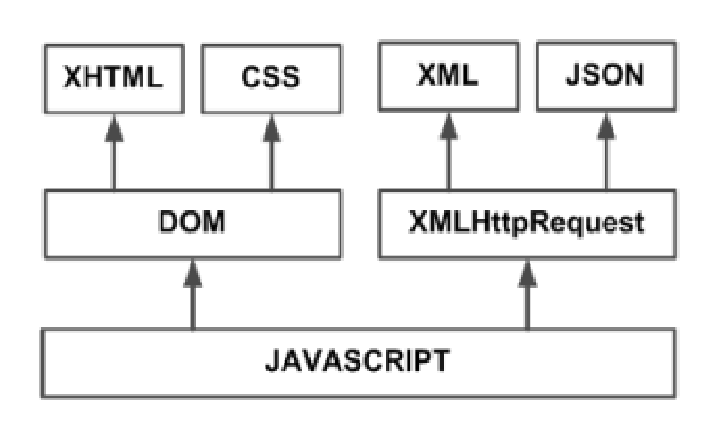
\includegraphics[width=9cm]{./eps/tecnologias/ajax_tecnologias_agrupadas.eps}
        \caption{Tecnologías agrupadas bajo el concepto de AJAX}
        \label{fig:tec_ajax_techs}
      \end{figure}
      
   El modelo clásico de aplicaciones Web funciona de esta forma: La mayoría de las acciones del usuario en la interfaz disparan un requerimiento HTTP al servidor web. El servidor efectúa un proceso (recopila información, procesa números, hablando con varios sistemas propietarios), y le devuelve una pagina HTLM al cliente.
   
   En la figura \ref{fig:tec_ajax_trad_vs_nuevo}, la imagen de la izquierda muestra el modelo tradicional de las aplicaciones web. La imagen de la derecha muestra el nuevo modelo propuesto por AJAX:
   
   \begin{figure}[H]
     \centering
       \includegraphics[width=10cm]{./eps/tecnologias/ajax_comparacion.eps}
     \caption{Comparación gráfica del modelo tradicional de aplicación web y del nuevo modelo propuesto por AJAX}
     \label{fig:tec_ajax_trad_vs_nuevo}
   \end{figure}   
   
   Esta técnica tradicional para crear aplicaciones web funciona correctamente, pero no crea una buena sensación al usuario. Al realizar peticiones continuas al servidor, el usuario debe esperar a que se recargue la página con los cambios solicitados. Si la aplicación debe realizar peticiones continuas, su uso se convierte en algo molesto

   AJAX permite mejorar completamente la interacción del usuario con la aplicación, evitando las recargas constantes de la página, ya que el intercambio de información con el servidor se produce en un segundo plano.

   Las aplicaciones construidas con AJAX eliminan la recarga constante de páginas mediante la creación de un elemento intermedio entre el usuario y el servidor. La nueva capa intermedia de AJAX mejora la respuesta de la aplicación, ya que el usuario nunca se encuentra con una ventana del navegador vacía esperando la respuesta del servidor.

   El siguiente esquema (figura \ref{fig:tec_ajax_comparaciones}) muestra la diferencia más importante entre una aplicación web tradicional y una aplicación web creada con AJAX. La imagen superior muestra la interación síncrona propia de las aplicaciones web tradicionales. La imagen inferior muestra la comunicación asíncrona de las aplicaciones creadas con AJAX.
   
   \begin{figure}[H]
      \centering
        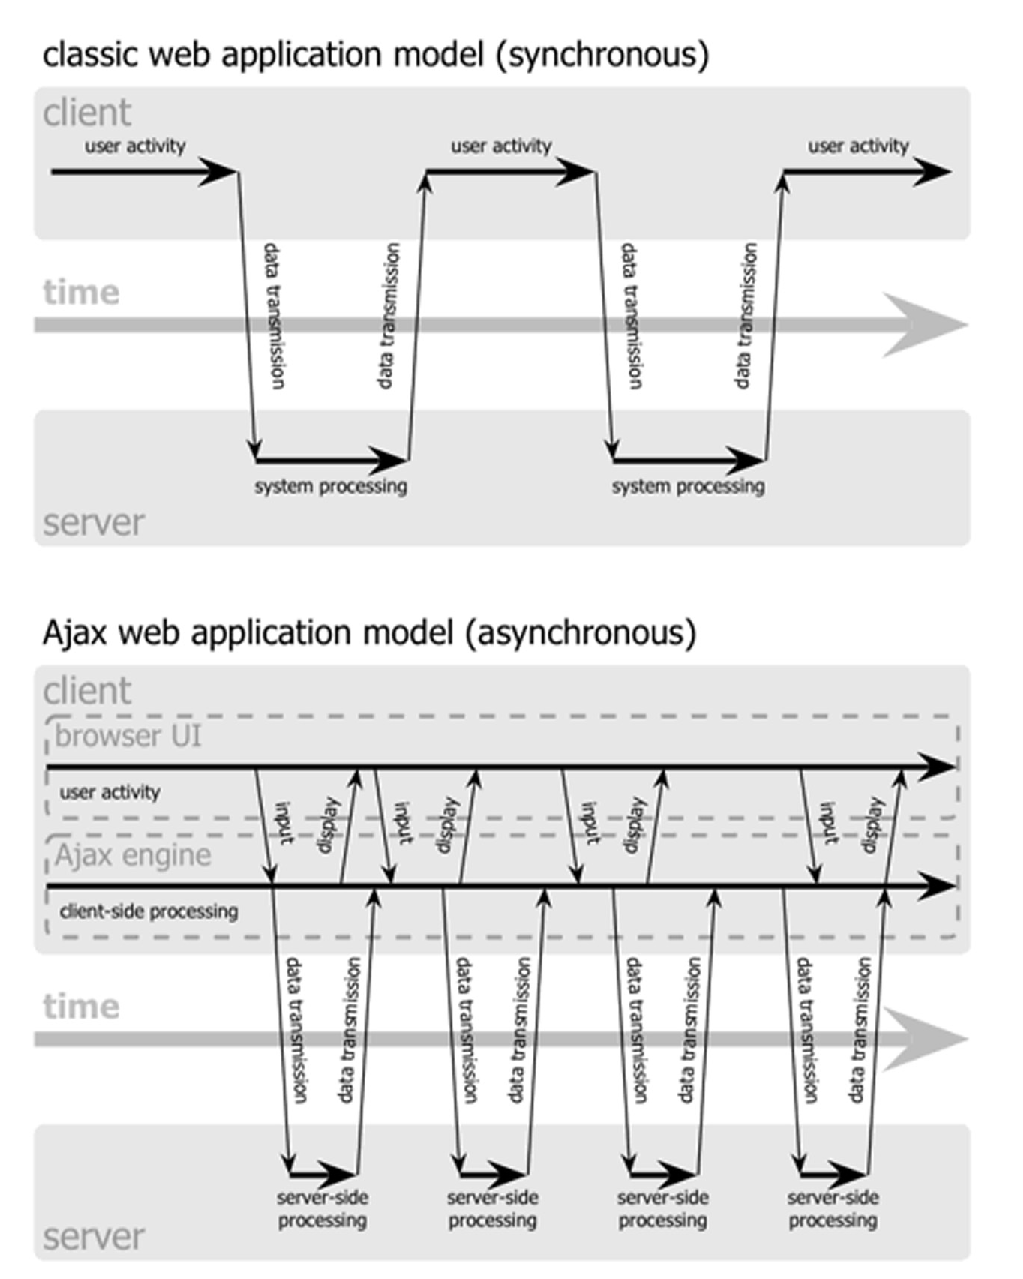
\includegraphics[width=10cm]{./eps/tecnologias/ajax_comunicaciones.eps}
      \caption{Comparación entre las comunicaciones síncronas de las aplicaciones web tradicionales y las comunicaciones asíncronas de las aplicaciones AJAX}
      \label{fig:tec_ajax_comparaciones}
    \end{figure}
    
    Las peticiones HTTP al servidor se sustituyen por peticiones JavaScript que se realizan al elemento encargado de AJAX. Las peticiones más simples no requieren intervención del servidor, por lo que la respuesta es inmediata. Si la interacción requiere una respuesta del servidor, la petición se realiza de forma asíncrona mediante AJAX. En este caso, la interacción del usuario tampoco se ve interrumpida por recargas de página o largas esperas por la respuesta del servidor.

    Desde su aparición, se han creado cientos de aplicaciones web basadas en AJAX. En la mayoría de casos, AJAX puede sustituir completamente a otras técnicas como Flash. Además, en el caso de las aplicaciones web más avanzadas, pueden llegar a sustituir a las aplicaciones de escritorio.
  
  % subsection ajax (end)
  
% section tecnologías (end)


%
% FIN DEL CAPÍTULO
%
\newpage
\thispagestyle{empty}
	%
% Capítulo 4 - Recursos/Herramientas necesarias
%
\chapter[Herramientas]{
	Herramientas
	\label{cap:herramientas}
}

Las distintas fases de trabajo del proyecto están apoyadas por un uso de software específico para su desarrollo.

Normalmente los proyectos software están desarrollados por equipos de trabajo de diversas magnitudes. Es esencial el uso de herramientas específicas que ayuden a automatizar tareas, ayudando a que el resto del equipo esté al tanto de las modificaciones realizadas.

\begin{center}{
	\fboxsep 10px
	\fcolorbox{white}{gray}{\parbox{0.95\textwidth}{
		Herramientas: RoR, latex, git, photoshop, textmate, aplicaciones web colaborativas, basecamp, pivotaltracker, jQuery, heroku
}}}\end{center}

% ----------------------------------
% Sec Ruby On Rails como framework Ruby
% ----------------------------------
\section{Ruby On Rails como framework Ruby} % (fold)
  \label{sec:ruby_on_rails_como_framework_ruby}
  
  {\it Ruby on Rails}, de ahora en adelante RoR, es una estructura de soporte para la programación web desarrollada en el lenguje Ruby por David Heinemeier Hansson, como resultado del desarrollo de {\it Basecamp} (un software para la gestión de proyectos vía web, basado en un interfaz sencillo, claro, fácil de usar, sin complicaciones). La primera versión del {\it framework} \footnote{Un {\bf framework} es una estructura conceptual y tecnológica de soporte definida, normalmente con artefactos o módulos de software concretos, con base en la cual otro proyecto de software puede ser organizado y desarrollado. Típicamente, puede incluir soporte de programas, bibliotecas y un lenguaje interpretado entre otros programas para ayudar a desarrollar y unir los diferentes componentes de un proyecto. Representa una arquitectura de software que modela las relaciones generales de las entidades del dominio. Provee una estructura y una metodología de trabajo la cual extiende o utiliza las aplicaciones del dominio.} salió a la luz pública en julio de 2004, así que RoR es muy reciente, y de ahí las reticencias que crea y la necesidad de analizar y hacer comparaciones sobre su utilidad respecto a otros soportes más consolidados.
  
  Para entender qué es RoR primero tenemos que conocer un poco en qué se apoya. RoR está programado en Ruby (ver referencias en sección \ref{sub:tec_ruby}). Los dos principios fundamentales sobre los cuáles se apoya RoR son, en primer lugar, «No te repitas» y, en segundo lugar, «Convenciones antes que configuración».
  
  % ----------------------------------
  % Sub No te repitas
  % ----------------------------------
  \subsection{No te repitas} % (fold)
    \label{sub:ror_no_te_repitas}
    
    DRY ({\it «Don't repeat yourself»}) significa que las definiciones sólo deben hacerse una vez. Como RoR es una estructura, los componentes están integrados de manera que ciertos «puentes» entre ellos no necesiten hacerse manualmente. Por ejemplo, si se tiene un formulario en la aplicación, con sólo una línea de código se puede llamar todas las veces que se quiera y donde quiera. 
    
    Otro ejemplo podría ser: en cada  tabla de la base de datos de la aplicación puedes manipular los registros de dicha tabla como si fueran atributos, sin necesidad de declarar nada, todo gracias al {\it Active Record}, uno de los patrones más llamativos de RoR.
    
    A veces, el lema «no te repitas» se expresa en otras palabras como «menos software». Menos software, menos código, significa dos cosas importantes: una es que el desarrollo se hace en menos tiempo y otra es que a menos código menos errores.
  % subsection no_te_repitas (end)
  
  % ----------------------------------
  % Sub Convenciones antes que configuración
  % ----------------------------------
  \subsection{Convenciones antes que configuración} % (fold)
    \label{sub:ror_convenciones_antes_que_configuracion}
    
    Convenciones antes que configuración significa que el programador sólo tiene que definir la configuración de aquello que no sea convencional. En muchas ocasiones definimos las cosas de la misma manera, hacemos las mismas configuraciones, con lo cual se tiende a repetir ciertos pasos una y otra vez. Estableciendo una serie de convecciones se logra ahorrar mucho tiempo porque el propio {\it framework}, por defecto, genera ciertos elementos. Por ejemplo, si se tiene en la aplicación una clase que se llama «Nadador» (nombre en singular), entonces gracias a las convenciones sabemos que en la base de datos existe una tabla que se llama «Nadadores» (nombre en plural), y así nos ahorramos escribir un montó de código a la hora de desarrollar la aplicación.
    
    Las convenciones existentes en Rails han sido definidas por el grupo de desarrolladores con la intención de facilitar el desarrollo, pero eso no implica que dichas convenciones no se puedan redefinir y cada cual configurarlas de otra manera y a su medida.
  % subsection convenciones_antes_que_configuración (end)

  % ----------------------------------
  % Sub Patrones de diseño
  % ----------------------------------
  \subsection{Patrones de diseño} % (fold)
    \label{sub:ror_patrones_de_diseno}
    
    Como se ha mencionado, {\it Ruby on Rails} es un {\it framework} para Ruby que implementa los patrones de diseño {\it Active Record} y Modelo-Vista-Controlador.
    
    % ----------------------------------
    % SubSub Active Record
    % ----------------------------------
    \subsubsection{Active Record} % (fold)
    \label{ssub:ror_active_record}
      
      {\it Active Record} es el patrón empleado por RoR para el Modelo, y soluciona el problema que surge cuando desde una programación orientada a objetos se quiere acceder a los datos de bases de datos relacionales. Con {\it Active Record}, el mapeo objeto-relacional se basa en unas pocas reglas muy sencillas: una tabla es una clase, una columna es un atributo, y una fila (tupla) es una instancia. Las relaciones entre tablas también siguen unas convenciones predefinidas: «tiene un» es una clave ajena, «tiene muchos» es una clave en otra tabla, «pertenece a» es una clave ajena y «muchos a muchos» es una tabla intermedia.
      
      El patrón {\it Active Record} permite salvar la distancia que existe entre el paradigma de la Programación Orientada a Objetos, que trata con objetos y asociaciones (paradigma más «natural»), y el modelo relacional, que trata con relaciones y conjuntos (modelo más matemático) cuando se trata de hacer persistentes los objetos del modelo de negocio.
    % subsubsection active_record (end)
    
    % ----------------------------------
    % SubSub Modelo-Vista-Controlador
    % ----------------------------------
    \subsubsection{Modelo-Vista-Controlador} % (fold)
    \label{ssub:modelo_vista_controlador}
    
    Este patrón soluciona el problema que surge cuando las vistas están acopladas a los modelos. Para desacoplarse se crea un tercer nivel que actúa como intermediación entre la Vista y el Modelo: el Controlador. El patrón MVC se basa en el principio general de desacoplar los objetos de modo que los cambios en un objeto afecten a otros pero sin necesidad de que el objeto que cambia conozco detalles de los otros.
    
    En RoR el modelo consiste en una serie de clases que representan las tablas de las bases de datos relacionales, siendo estas clases gestionadas por {\it Active Record}. La Vista es la visualización de los datos que se manejan desde las clases de los {\it Controller}. Los ficheros de la Vista tienen una extensión {\i rhtml} (puede modificarse), y contienen código Ruby embebido en HTML.
    
    Para la construcción de estos tres niveles (Modelo, Vista y Controlador), RoR ofrece un andamiaje: es lo que se llama «scaffolding». {\it Scaffolding} consiste en la construcción automática de todo el código del Modelo y de las Vistas que se necesitan para realizar las operaciones más frecuentes, como puede ser crear nuevos nadadores, ver los nadadores ya existentes, modificarlos o borrarlos, etc. Los responsables de la generación de este código son los «Scaffold Generators», generadores automáticos de código que facilitan la creación de requisitos «CRUD» (Create, Read, Update y Delete) basados en formularios web y con operaciones necesarios para el manejo de registros.
    
    % subsubsection modelo_vista_controlador (end)
  % subsection patrones_de_diseño (end)
  
  % ----------------------------------
  % Sub Servicios RESTful
  % ----------------------------------
  \subsection{Servicios RESTful} % (fold)
    \label{sub:servicios_restful}
    
    REST define un set de principios arquitectónicos por los cuales se diseñan servicios web haciendo foco en los recursos del sistema, incluyendo cómo se accede al estado de dichos recursos y cómo se transfieren por HTTP hacia clientes escritos en diversos lenguajes. REST emergió en los últimos años como el modelo predominante para el diseño de servicios. De hecho, REST logró un impacto tan grande en la web que prácticamente logró desplazar a SOAP \footnote{{\bf SOAP} (siglas de {\it Simple Object Access Protocol}) es un protocolo estándar que define cómo dos objetos en diferentes procesos pueden comunicarse por medio de intercambio de datos XML} y las interfaces basadas en WSDL \footnote {{\bf WSDL} (siglas de {\it Web Services Description Language}), un formato XML que se utiliza para describir servicios Web } por tener un estilo bastante más simple de usar.

    REST no tuvo mucha atención cuando Roy Fielding lo presentó por primera vez en el año 2000 en la Universidad de California, durante la charla academica «Estilos de Arquitectura y el Diseño de Arquitecturas de Software basadas en Redes», la cual analizaba un conjunto de principios arquitectónicos de software para usar a la Web como una plataforma de Procesamiento Distribuido.
  
    % ----------------------------------
    % SubSub Principios de REST
    % ----------------------------------
    \subsubsection{Principios de REST} % (fold)
    \label{ssub:ror_principios_de_rest}
      
      Una implementación concreta de un servicio web REST sigue cuatro principios de diseño fundamentales:
      
      \begin{enumerate}
        \item Utiliza los métodos HTTP de manera explícita
        \item No mantiene estado
        \item Expone URIs con forma de directorios
        \item Transfiere XML, JavaScript Object Notation (JSON), o ambos
      \end{enumerate}

      A continuación vamos a ver en detalle estos cuatro principios, y explicaremos porqué son importantes a la hora de diseñar un servicio web REST.
      
      \paragraph{Utiliza los métodos HTTP de manera explícita.} % (fold)
      \label{par:utiliza_los_metodos_http_de_manera_explicita}
        Una de las características claves de los servicios web REST es el uso explícito de los métodos HTTP, siguiendo el protocolo definido por RFC 2616. Por ejemplo, HTTP GET se define como un método productor de datos, cuyo uso está pensado para que las aplicaciones cliente obtengan recursos, busquen datos de un servidor web, o ejecuten una consulta esperando que el servidor web la realice y devuelva un conjunto de recursos.

        REST hace que los desarrolladores usen los métodos HTTP explícitamente de manera que resulte consistente con la definición del protocolo. Este principio de diseño básico establece una asociación uno-a-uno entre las operaciones de crear, leer, actualizar y borrar y los métodos HTTP. De acuerdo a esta asociación:

        \begin{itemize}
          \item Se usa POST para crear un recurso en el servidor
          \item Se usa GET para obtener un recurso
          \item Se usa PUT para cambiar el estado de un recurso o actualizarlo
          \item Se usa DELETE para eliminar un recurso 
        \end{itemize}
      % paragraph utiliza_los_métodos_http_de_manera_explícita (end)
  
      \paragraph{No mantiene estado.} % (fold)
      \label{par:no_mantiene_estado}
        Los servicios web REST necesitan escalar para poder satisfacer una demanda en constante crecimiento. Se usan clusters de servidores con balanceadores de carga y alta disponibilidad, {\it proxies}, y {\it gateways} de manera de conformar una topología serviciable, que permita transferir peticiones de un equipo a otro para disminuir el tiempo total de respuesta de una invocación al servicio web. El uso de servidores intermedios para mejorar la escalabilidad hace necesario que los clientes de servicios web REST envíen peticiones completas e independientes; es decir, se deben enviar peticiones que incluyan todos los datos necesarios para cumplir el pedido, de manera que los componentes en los servidores intermedios puedan redireccionar y gestionar la carga sin mantener el estado localmente entre las peticiones.

        Una petición completa e independiente hace que el servidor no tenga que recuperar ninguna información de contexto o estado al procesar la petición. Una aplicación o cliente de servicio web REST debe incluir dentro del encabezado y del cuerpo HTTP de la petición todos los parámetros, contexto y datos que necesita el servidor para generar la respuesta. De esta manera, el no mantener estado mejora el rendimiento de los servicios web y simplifica el diseño e implementación de los componentes del servidor, ya que la ausencia de estado en el servidor elimina la necesidad de sincronizar los datos de la sesión con una aplicación externa.
      % paragraph no_mantiene_estado (end)
      
      \paragraph{Expone URIs con forma de directorios.} % (fold)
      \label{par:expone_uris_con_forma_de_directorios}
      
      Desde el punto de vista del cliente de la aplicación que accede a un recurso, la URI determina qué tan intuitivo va a ser el web service REST, y si el servicio va a ser utilizado tal como fue pensado al momento de diseñarlo. La tercera característica de los servicios web REST es justamente sobre las URIs.

      Las URI de los servicios web REST deben ser intuitivas, hasta el punto de que sea facil adivinarlas. Pensemos en las URI como una interfaz auto-documentada que necesita de muy poca o ninguna explicación o referencia para que un desarrollador pueda comprender a lo que apunta, y a los recursos derivados relacionados.

      Una forma de lograr este nivel de usabilidad es definir URIs con una estructura al estilo de los directorios. Este tipo de URIs es jerárquica, con una única ruta raíz, y va abriendo ramas a través de las subrutas para exponer las áreas principales del servicio. De acuerdo a esta definición, una URI no es sólamente una cadena de caracteres delimitada por barras, sino más bien un árbol con subordinados y padres organizados como nodos.
      
      % paragraph expone_uris_con_forma_de_directorios_ (end)
      
      \paragraph{REST transfiere XML, JSON, o ambos.} % (fold)
      \label{par:rest_transfiere_xml_json_o_ambos}
        La representación de un recurso en general refleja el estado actual del mismo y sus atributos al momento en que el cliente de la aplicación realiza la petición. La representación del recurso son simples «fotos» en el tiempo. Esto podría ser una representación de un registro de la base de datos que consiste en la asociación entre columnas y tags XML, donde los valores de los elementos en el XML contienen los valores de las filas. O, si el sistema tiene un modelo de datos, la representación de un recurso es una fotografía de los atributos de una de las cosas en el modelo de datos del sistema. 

        La última restricción al momento de diseñar un servicio web REST tiene que ver con el formato de los datos que la aplicación y el servicio intercambian en las peticiones/respuestas. Acá es donde realmente vale la pena mantener las cosas simples, legibles por humanos, y conectadas.

        Los objetos del modelo de datos generalmente se relacionan de alguna manera, y las relaciones entre los objetos del modelo de datos (los recursos) deben reflejarse en la forma en la que se representan al momento de transferir los datos al cliente.
      
      % paragraph rest_transfiere_xml_json_o_ambos_ (end)
      
    % subsubsection principios_de_rest (end)
  
  % subsection servicios_restful (end)

% section ruby_on_rails_como_framework_ruby (end)

% ----------------------------------
% Sec jQuery como framework Javascript
% ----------------------------------
\section{jQuery como framework Javascript} % (fold)
  \label{sec:jquery_como_framework_javascript}

  jQuery es un framework de JavaScript, creada inicialmente por John Resig, que permite simplificar la manera de interactuar con los documentos HTML, manipular el árbol DOM, manejar eventos, desarrollar animaciones y agregar interacción con la técnica AJAX a páginas web.
  
  jQuery es software libre y de código abierto, posee un doble licenciamiento bajo la Licencia MIT y la Licencia Pública General de GNU v2, permitiendo su uso en proyectos libres y privativos. Al igual que otras bibliotecas, ofrece una serie de funcionalidades basadas en JavaScript que de otra manera requerirían de mucho más código, es decir, con las funciones propias de esta biblioteca se logran grandes resultados en menos tiempo y espacio.
  
  Entre las ventajas de uso se encuentran:
  
    \begin{itemize}
      \item {\bf Buena aceptación} por parte de los desarrolladores.
      \item {\bf Compatibilidad}. Cuando un desarrollador tiene que utilizar Javascript, generalmente tiene que preocuparse por hacer scripts compatibles con varios navegadores y para ello tiene que incorporar mucho código que lo único que hace es detectar el navegador del usuario, para hacer una u otra cosa dependiendo de si es Internet Explorer, Firefox, Opera, etc. jQuery es donde más nos puede ayudar, puesto que implementa una serie de clases (de programación orientada a objetos) que nos permiten programar sin preocuparnos del navegador con el que nos está visitando el usuario, ya que funcionan de exacta forma en todas las plataformas más habituales.
      \item {\bf Licencia gratuita}. El framework tiene licencia para uso en cualquier tipo de plataforma, personal o comercial.
      \item {\bf Liviano}. El archivo del framework ocupa unos 56 KB (19KB en caso de enviarse de manera comprimida), lo que es bastante razonable y no retrasará mucho la carga de las páginas que intervienen en el proyecto. El servidor lo enviará al cliente la primera vez que visite una página del sitio. En siguientes páginas el cliente ya tendrá el archivo del framework, por lo que no necesitará transferirlo y lo tomará de la caché. Con ello, la carga de la página sólo se verá afectada por el peso de este framework una vez por usuario. Las capacidades que ofrece el paquete compensan extraordinariamente el peso del paquete.
      \item {\bf Estabilidad y buena documentación}. Cuenta con un gran equipo de desarrolladores a cargo de mejoras y actualizaciones del framework, junto con una comunidad que ayuda a encontrar soluciones.
    \end{itemize}
    
  Sus principales características:
  
  \begin{itemize}
    \item Selección de elementos DOM.
    \item Interactividad y modificaciones del árbol DOM, incluyendo soporte para CSS 1-3.
    \item Eventos.
    \item Manipulación de la hoja de estilos CSS.
    \item Efectos y animaciones.
    \item Animaciones personalizadas.
    \item AJAX.
    \item Soporta extensiones.
    \item Utilidades varias como obtener información del navegador, operar con objetos y vectores, funciones como {\it trim()} (elimina los espacios en blanco del principio y final de una cadena de caracteres), etc.
    \item Compatible con los navegadores Mozilla Firefox 2.0+, Internet Explorer 6+, Safari 3+, Opera 10.6+ y Google Chrome 8+.
  \end{itemize}  
  
% section jquery_como_framework_javascript (end)

% ----------------------------------
% Sec Latex como procesador de texto
% ----------------------------------
\section{Latex como procesador de texto} % (fold)
  \label{sec:latex_como_procesador_de_texto}
  
  {\it LaTeX} es un sistema de composición de textos que está formado mayoritariamente por órdenes (macros) construidas a partir de comandos de TeX —un lenguaje «de bajo nivel», en el sentido de que sus acciones últimas son muy elementales— pero con la ventaja añadida, en palabras de Lamport, de «poder aumentar las capacidades de LaTeX utilizando comandos propios del TeX descritos en The TeXbook». Esto es lo que convierte a LaTeX en una herramienta práctica y útil pues, a su facilidad de uso, se une toda la potencia de TeX. Estas características hicieron que LaTeX se extendiese rápidamente entre un amplio sector científico y técnico, hasta el punto de convertirse en uso obligado en comunicaciones y congresos, y requerido por determinadas revistas a la hora de entregar artículos académicos.
  
  Su código abierto permitió que muchos usuarios realizasen nuevas utilidades que extendiesen sus capacidades con objetivos muy variados, a veces ajenos a la intención con la que fue creado: aparecieron diferentes dialectos de LaTeX que, a veces, eran incompatibles entre sí. Para atajar este problema, en 1989 Lamport y otros desarrolladores iniciaron el llamado «Proyecto LaTeX3». En el otoño boreal de 1993 se anunció una re-estandarización completa de LaTeX, mediante una nueva versión que incluía la mayor parte de estas extensiones adicionales (como la opción para escribir transparencias o la simbología de la American Mathematical Society) con el objetivo de dar uniformidad al conjunto y evitar la fragmentación entre versiones incompatibles de LaTeX 2.09. Esta tarea la realizaron Frank Mittlebach, Johannes Braams, Chris Rowley y Sebastian Rahtz junto al propio Leslie Lamport. Hasta alcanzar el objetivo final del «Proyecto 3», a las distintas versiones se las viene denominando  (o sea, «versión 2 y un poco más»). Actualmente cada año se ofrece una nueva versión, aunque las diferencias entre una y otra suelen ser muy pequeñas y siempre bien documentadas.
  
  Con todo, además de todas las nuevas extensiones, la característica más relevante de este esfuerzo de re-estandarización fue la arquitectura modular: se estableció un núcleo central (el compilador) que mantiene las funcionalidades de la versión anterior pero permite incrementar su potencia y versatilidad por medio de diferentes paquetes que solo se cargan si son necesarios. De ese modo, LaTeX dispone ahora de innumerables paquetes para todo tipo de objetivos, muchos dentro de la distribución oficial, y otros realizados por terceros, en algunos casos para usos especializados.

  % ----------------------------------
  % Sub Uso
  % ----------------------------------
  \subsection{Uso} % (fold)
    \label{sub:uso}
    
    LaTeX presupone una filosofía de trabajo diferente a la de los procesadores de texto habituales (conocidos como WYSIWYG, es decir, «lo que ves es lo que obtienes») y se basa en comandos. Tradicionalmente, este aspecto se ha considerado una desventaja (probablemente la única). Sin embargo, LaTeX, a diferencia de los procesadores de texto de tipo WYSIWYG, permite a quien escribe un documento centrarse exclusivamente en el contenido, sin tener que preocuparse de los detalles del formato. Además de sus capacidades gráficas para representar ecuaciones, fórmulas complicadas, notación científica e incluso musical, permite estructurar fácilmente el documento (con capítulos, secciones, notas, bibliografía, índices analíticos, etc.), lo cual brinda comodidad y lo hace útil para artículos académicos y libros técnicos.
    
    Con LaTeX, la elaboración del documento requiere normalmente de dos etapas: en la primera hay que crear mediante cualquier editor de texto llano un fichero fuente que, con las órdenes y comandos adecuados, contenga el texto que queramos imprimir. La segunda consiste en procesar este fichero; el procesador de textos interpreta las órdenes escritas en él y compila el documento, dejándolo preparado para que pueda ser enviado a la salida correspondiente, ya sea la pantalla o la impresora. Ahora bien, si se quiere añadir o cambiar algo en el documento, se deberá hacer los cambios en el fichero fuente y procesarlo de nuevo. Esta idea, que puede parecer poco práctica a priori, es conocida a los que están familiarizados con el proceso de compilación que se realiza con los lenguajes de programación de alto nivel, ya que es completamente análogo.
    
    El modo en que LaTeX interpreta la «forma» que debe tener el documento es mediante etiquetas. Puede resultar extraño que hoy en día se siga usando algo que no es WYSIWYG, pero las características de LaTeX siguen siendo muchas y muy variadas. También hay varias herramientas (aplicaciones) que ayudan a una persona a escribir estos documentos de una manera más visual (LyX, TeXmacs y otros). A estas herramientas se les llama WYSIWYM («lo que ves es lo que quieres decir»).
    
    Una de las ventajas de LaTeX es que la salida que ofrece es siempre la misma, con independencia del dispositivo (impresora, pantalla) o el sistema operativo (MS Windows, MacOS, Unix, GNU/Linux) y puede ser exportado a partir de una misma fuente a numerosos formatos tales como Postscript, PDF, SGML, HTML o RTF. Existen distribuciones e IDEs de LaTeX para todos los sistemas operativos más extendidos, que incluyen todo lo necesario para trabajar. Hay, por ejemplo, programas para Windows como TeXnicCenter, para Linux como Kile, o para MacOS como TeXShop, todos liberados bajo la Licencia GPL. Existe además un editor multiplataforma (para MacOS, Windows y Unix) llamado Texmaker, que también tiene licencia GPL.
  % subsection uso (end)
  
  % ----------------------------------
  % Sub Ventajas y desventajas
  % ----------------------------------
  \subsection{Ventajas y desventajas} % (fold)
    \label{sub:latex_ventajas_y_desventajas}
    
    Cuando gente del mundo WYSIWYG se encuentra con usuarios de LaTeX, a menudo discuten «las ventajas de LaTeX sobre un procesador de textos normal» o lo contrario. Las principales ventajas de LaTeX sobre procesadores de texto normales son las siguientes:
    
    \begin{itemize}
      \item Se dispone de composiciones diseñadas profesionalmente, lo que hace que un documento parezca realmente «impreso».
      \item El soporte para la composición de fórmulas matemáticas es muy adecuado.
      \item Los usuarios sólo tienen que aprender unas pocas órdenes fáciles de entender, que especifican la estructura lógica del documento. Casi nunca necesitan preocuparse del aspecto real del documento.
      \item Es fácil generar incluso estructuras complejas, como notas al pie, referencias, índices o bibliografías.
      \item Existen paquetes libres (incluso gratuitos) que facilitan muchas tareas tipográficas especializadas, no soportadas directamente por el LaTeX básico. Por ejemplo, hay disponibles paquetes para incluir gráficos o para componer bibliografías según normas precisas. se describen muchos de estos paquetes en {\it The LaTeX Companion}.\cite{LATCOMP04}
      \item LaTeX incita a los autores a escribir textos bien estructurados, porque así trabaja LaTeX ---especificando la estructura---.
      \item TeX, el motor de formateo de LaTeX, es libre y muy portable. Por tanto, puede ejecutarse en casi cualquier plataforma informática disponible.
    \end{itemize}
    
    LaTeX tiene también algunas desventajas, entre las cuales se pueden mencionar:
    
    \begin{itemize}
      \item La curva de aprendizaje para aquellas personas que están muy acostumbrados a procesadores WYSIWYG y que no está familiarizados con textos planos es alta.
      \item Aunque pueden ajustarse algunos parámetros dentro de una cierta composición del documento, el diseño de una nueva composición completa es difícil y lleva mucho tiempo.
      \item Es muy duro escribir documentos desestructurados y desorganizados.
      \item Puede ser duro comprender el concepto de marcado lógico para personas que no están acostumbradas a trabajar con lenguajes de programación.
    \end{itemize}
  
  % subsection ventajas_y_desventajas (end)
% section latex_como_procesador_de_texto (end)

% ------------------------------------------
% Sec Git como sistema de control de versiones
% ------------------------------------------
\section{Git como sistema de control de versiones}

\subsection{Acerca del control de versiones}
¿Qué es el control de versiones, y por qué debería importar? Una versión, revisión o edición de un producto, es el estado en el que se encuentra dicho producto en un momento dado de su desarrollo o modificación. Se llama {\bf control de versiones} a la gestión de los diversos cambios que se realizan sobre los elementos de algún producto o una configuración del mismo, de modo que se puedan recuperar versiones específicas más adelante. Los sistemas de control de versiones facilitan la administración de las distintas versiones de cada producto desarrollado, así como las posibles especializaciones realizadas.

El control de versiones se realiza principalmente en la industria informática para controlar las distintas versiones del código fuente. Sin embargo, los mismos conceptos son aplicables a otros ámbitos como documentación, imágenes o sitios web.

\subsubsection{Sistemas de control de versiones distribuidos}

En los sistemas de control de versiones distribuidos (figura \ref{fig:cvdistrib}), Los clientes no sólo descargan la última instantánea de los archivos: replican completamente el repositorio. Así, si un servidor muere, y estos sistemas estaban colaborando a través de él, cualquiera de los repositorios de los clientes puede copiarse en el servidor para restaurarlo. Cada vez que se descarga una instantánea, en realidad se hace una copia de seguridad completa de todos los datos

\begin{figure}[H]
  \centering
    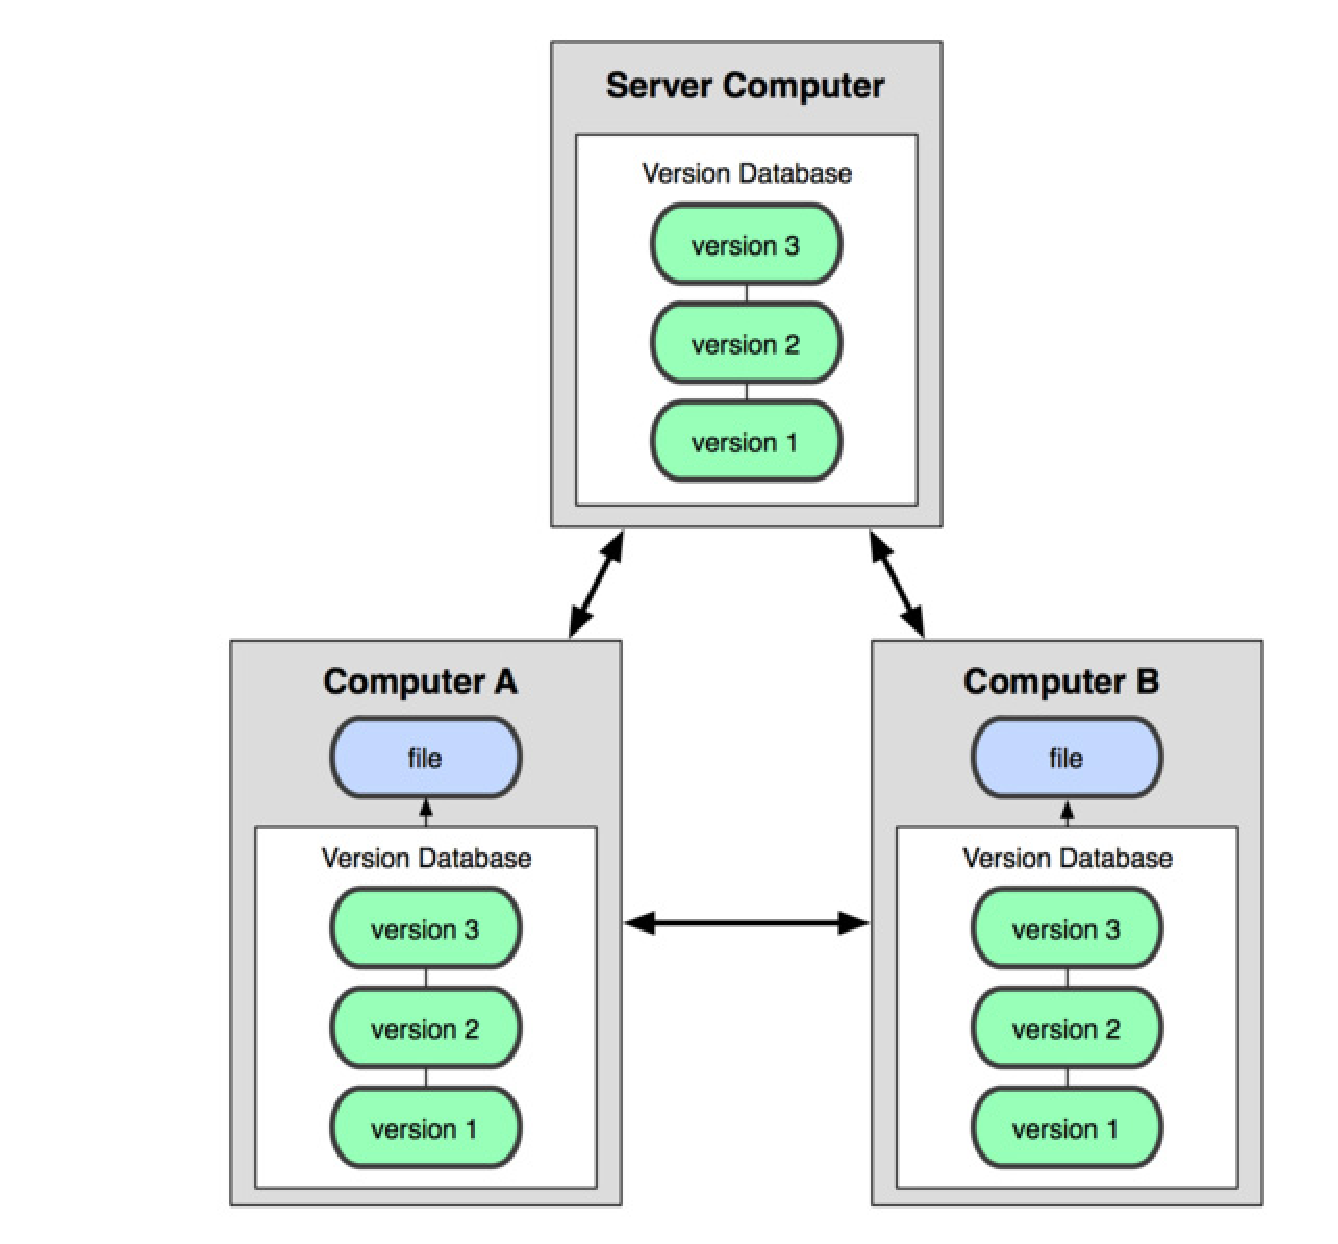
\includegraphics[width=300px]{./eps/git/git_diag_cv_distribuido.eps}
  \caption{Diagrama de control de versiones distribuido}
  \label{fig:cvdistrib}
\end{figure}

\subsection{Acerca de Git}

Debido al fuerte apoyo de la comunidad y su gran uso comercial, se selecciona como herramienta para la gestión de versiones. Así mismo, se han analizado sus ventajas frente a SVN (capítulo \ref{sec:git_vs_svn} en apéndice \fullref{ap:git})

Git (referencia en apéndice \fullref{ap:git}) es un software de control de versiones diseñado por Linus Torvalds, pensando en la eficiencia y la confiabilidad del mantenimiento de versiones de aplicaciones cuando estas tienen un gran número archivos de código fuente. Al principio, Git se pensó como un motor de bajo nivel sobre el cual otros pudieran escribir la interfaz de usuario o front-end. Sin embargo, Git se ha convertido desde entonces en un sistema de control de versiones con funcionalidad plena. Hay algunos proyectos de mucha relevancia que ya usan Git, en particular, el grupo de programación del núcleo Linux.

El flujo de trabajo básico en Git es:
\begin{enumerate}
	\item{Modificar una serie de archivos en directorio de trabajo.}
	\item{Preparar los archivos, añadiendo instantáneas de ellos al área de preparación.}
	\item{Confirmar los cambios, lo que toma los archivos tal y como están en el área de preparación, y almacena esa instantánea de manera permanente en el directorio de Git remoto.}
\end{enumerate}
	

% Características de Git
\subsubsection {Características}

El diseño de Git se basó en BitKeeper \footnote{BitKeeper es el sistema de gestion de codigo fuente usado en inicios para el kernel de Linux. BitMover (el fabricante) decidió no mantener la versión gratuita por motivos de rentabilidad económica.} y en Monotone. 
Sus principales características son:

\begin{itemize}
	\item{
		Fuerte apoyo al desarrollo no-lineal, por ende rapidez en la gestión de ramificaciones y mezclado de diferentes versiones. Git incluye herramientas específicas para navegar y visualizar un historial de desarrollo no-lineal. Una presunción medular en Git es que un cambio será fusionado mucho más frecuentemente de lo que se escribe originalmente, conforme se pasa entre varios programadores que lo revisan.
	}
	\item{
		Gestión distribuida. Git le da a cada programador una copia local del historial del desarrollo entero, y los cambios se propagan entre los repositorios locales. Los cambios se importan como ramificaciones adicionales y pueden ser fusionados en la misma manera que se hace con la ramificación local.
	}
	\item{
		Los almacenes de información pueden publicarse por HTTP, FTP, rsync o mediante un protocolo nativo, ya sea a través de una conexión TCP/IP simple o a través de cifrado SSH. Git también puede emular servidores CVS, lo que habilita el uso de clientes CVS pre-existentes y modulos IDE para CVS pre-existentes en el acceso de repositorios Git.
	}
	\item{
	 	Los repositorios Subversion y SVK se pueden usar directamente con git-svn.
	}
	\item{
		Gestión eficiente de proyectos grandes, dada la rapidez de gestión de diferencias entre archivos, entre otras mejoras de optimización de velocidad de ejecución.
	}
	\item{
		Todas las versiones previas a un cambio determinado, implican la notificación de un cambio posterior en cualquiera de ellas a ese cambio (denominado autenticación criptográfica de historial).
	}
\end{itemize}


% ----------------------------------
% Sec Textmate como editor de textos
% ----------------------------------
\section{Textmate como editor de textos} % (fold)
  \label{sec:textmate_como_editor_de_textos}
  
  Probablemente, la herramienta de software con la que pasemos más tiempo en nuestro trabajo diario como programadores sea el editor de código. Es por ello que la importancia de elegir un buen editor se convierte en primordial, y es probablemente una de las selecciones más cuidadosas que debemos hacer si queremos que nuestra productividad no sufra.

  Textmate es un editor de textos de pago con interfaz GUI para Mac OS X, creado por Allan Odgaard. La ventaja principal ante usar entornos de programación específicos es que es un editor altamente personalizable, que consume muy pocos recursos y que es capaz de soportar la compilación de diferentes lenguajes. Además, cuenta con ayudas de teclado (conocidas como «macros») para aumentar la productividad de programación. 

  No es un IDE, es decir, no pretende abarcar todas y cada una de las posibilidades que contemple tu plataforma de desarrollo. Pero lo cierto es que gracias a las extensiones en forma de {\it snippets} de código, macros, y otros, se puede convertir perfectamente en el centro de control absoluto durante el desarrollo de tu proyecto. Y todo esto siendo muchísimo más ligero que los tradicionales IDE, con la ventaja adicional de ser agnóstico (no todos los IDE lo son) en cuanto a las herramientas extra que estemos usando: compilador, sistema de control de versiones, etc.  

  Algunas de las características más destacadas de este editor son:
  
  \begin{itemize}
    \item Búsqueda y reemplazo de texto en un proyecto (ideal para refactorizaciones).
    \item Búsqueda y reemplazo de texto por expresiones regulares.
    \item Autoindentado en acciones comunes, como pegar texto.
    \item Autoemparejado de corchetes y otros caracteres.
    \item Histórico del portapapeles.
    \item Selector de texto por columnas y escritura en varias líneas a la vez en una misma columna (ideal para añadir un prefijo común a varias líneas de código, por ejemplo).
    \item Autocompletado de palabras de entre las que aparecen en el documento actual.
    \item Selectores para limitar el alcance de las acciones y las preferencias del editor.
    \item Bloques de código plegables.
    \item Grabación de macros (para crearlas sin necesidad de programarlas).
    \item Cambio rápido a cualquier fichero del proyecto tecleando parte de su nombre.
    \item Ejecutar comandos del sistema en el contexto de un documento.
    \item Navegación entre ficheros por pestañas.
    \item Soporte para más de 50 lenguajes.
    \item Soporte para casi todos los sistemas de control de versiones.
    \item Personalización del editor a través de temas.
  \end{itemize}

  % ----------------------------------
  % Sub Snippets
  % ----------------------------------
  \subsection{Snippets} % (fold)
    \label{sub:textmate_snippets}
  
    Los {\it snippets} permiten insertar porciones de código en el fichero que se esté editando de forma muy sencilla y moverse rápidamente por el texto personalizable de dicho {\it snippet}. Se pueden contextualizar, de modo que ciertos {\it snippets} sólo se puedan utilizar si se está editando un determinado tipo de fichero.

    Los {\it snippets} son accesibles desde la opción de menú {\it Bundles}, donde están ordenados por contexto (habitualmente, el lenguaje o entorno de programación que se esté usando). Aunque lo mejor es lanzarlos creando para ellos una secuencia de caracteres, tras las que, al pulsar tabulador, se ejecuta.

  % subsection snippets (end)
  
  % ----------------------------------
  % Sub Comandos
  % ----------------------------------
  \subsection{Comandos} % (fold)
    \label{sub:textmate_comandos}
    
    Los comandos en TextMate permiten ejecutar un código arbitrario (definido por una extensión en particular), el cual puede estar escrito en un lenguaje de programación. TextMate define una serie de variables de entorno con información como la línea actual, la ruta al proyecto, el fichero que se está editando, el texto seleccionado, etc. El comando sólo tiene que tomar la información que necesite y actuar en consecuencia. El resultado de ejecutar dicho comando puede introducirse directamente en el punto donde estaba situado el cursor, reemplazar todo o parte del texto, crear un nuevo documento y pegarse en él, etc.

    Los comandos son accesibles también desde el menú {\it Bundles}, o se pueden asignar a la pulsación de ciertas teclas para que se lancen. Su activación puede depender de que estés en el contexto adecuado, de modo que puedes usar la misma combinación de teclas para distintos comportamientos según estés editando código en Ruby, en C o en Java. 
    
  % subsection comandos (end)

% section textmate_como_editor_de_textos (end)

% ----------------------------------
% Sec PivotalTracker como gestor de proyectos ágiles
% ----------------------------------
\section{Pivotal Tracker como gestor de proyectos ágiles} % (fold)
  \label{sec:pivotaltracker_como_gestor_de_proyectos_agiles}

  Es una herramienta gratuita de {\bf Pivotal Labs}. Está destinada a la gestión de proyectos ágiles, permitiendo organizar las tareas utilizando el concepto de gestión de pilas.
  
  La herramienta es recomendable para los desarrolladores y coordinadores de proyectos, así como para los clientes y agentes externos. La curva de aprendizaje es muy sencilla, lo cuál permite tomar esta herramienta en cualquier momento y probarla sin tener un costo adicional en cuanto a pérdida de tiempo.

  Cuenta con diversas fuentes de información y métricas para controlar, de una forma detallada, el progreso diario, semanal y mensual de un proyecto o de sus miembros.
  
  % ----------------------------------
  % Sub Familiarización con el entorno
  % ----------------------------------
  \subsection{Familiarización con el entorno} % (fold)
    \label{sub:familiarizacion_con_el_entorno}
    
    En las sucesivas secciones se detallará el uso de la aplicación para la gestión de los proyectos, así como se introducirá al lector para que pueda familiarizarse con la misma.
    
    % ----------------------------------
    % SubSub Pilas
    % ----------------------------------
    \subsubsection{Pilas} % (fold)
    \label{ssub:pilas}
      Las historias de usuario, que se asemejan a las tareas de cada uno de los requisitos que se desarrollará, se ordenan en distintas columnas denominadas {\bf pilas}. Hay 4 tipos de pilas:
      \begin{itemize}
        \item {\bf Current}. Historias de usuario planificadas para la iteración en la que estamos.
        \item {\bf Backlog}. Historias de usuario planificadas para iteraciones futuras. {\it Pivotal Tracker} define donde empiezan las iteraciones según la velocidad establecida. Con esto se puede conseguir una estimación a largo plazo del proyecto.
        \item {\bf Icebox}. Historias de usuario que algún día quizás se realicen. Por defecto, cuando se crea una historia nueva, se coloca en esta pila.
        \item {\bf Done}. Normalmente no se muestra. Se muestras las iteraciones pasadas. 
      \end{itemize}
      
      \begin{figure}[H]
        \centering
          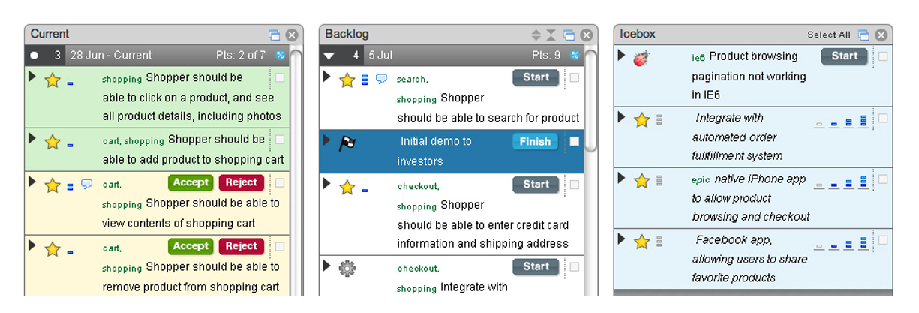
\includegraphics[width=15cm]{./eps/herramientas/pt/pt_pilas.eps}
        \caption{Tipos de pilas en Pivotal Tracker}
        \label{fig:pt_pilas}
      \end{figure}
      
    % subsubsection pilas (end)
  
    % ----------------------------------
    % SubSub Tipos de historias de usuario
    % ----------------------------------
    \subsubsection{Tipos de historias de usuario} % (fold)
    \label{ssub:tipos_de_historias_de_usuario}
      
      \begin{itemize}
        \item {\bf Feature}. Representadas por una estrella. Representan requisitos de usuario y las única que estiman (aportan valor de negocio al usuario). La velocidad se debería medir en funcionalidad de negocio capaz de realizar en una iteración).
        \item {\bf Bugs}. Modificaciones que hay realizar para mejorar un error.
        \item {\bf Chore} (trabajo rutinario). Representan tareas que hay que hacer y que no aportan valor de negocio ni son errores.
        \item {\bf Release}. Marcan hitos en el tiempo. Se tienen en cuenta en la planificación y en el cálculo de velocidad. Cuando se crea una release, se indica la fecha: si todo va bien saldrá en azul, pero si según la velocidad definida no dará tiempo a terminar todas las historias que hay por delante, se marcará en rojo.
      \end{itemize}
      
      \begin{figure}[H]
        \centering
          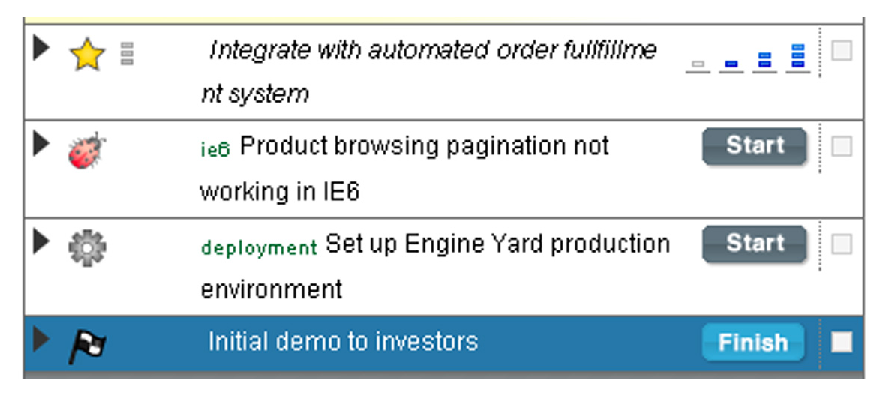
\includegraphics[width=11cm]{./eps/herramientas/pt/pt_historias.eps}
        \caption{Tipos de historias de usuario en Pivotal Tracker}
        \label{fig:pt_historias}
      \end{figure}
      
      Cada historia se puede modificar estableciendo el tipo, estimación de velocidad, etiquetas, estado, miembro, descripción, comentario y archivos adjuntos.
    % subsubsection tipos_de_historias_de_usuario (end)
    
    % ----------------------------------
    % SubSub Tipos de estados en historias
    % ----------------------------------
    \subsubsection{Tipos de estados en historias} % (fold)
    \label{ssub:tipos_de_estados_en_historias}
    
      Los estados vienen definidos por:
      \begin{itemize}
        \item {\bf Not Yet Started}. Todavía no se ha empezado a trabajar sobre la historia. Puede estar en cualquier pila menos {\it «done»}. 
        \item {\bf Started}. Se refiere a las historias comenzadas, es decir, en la que se está actualmente trabajando. Si dede cualquier pila se pulsa el botón de {\it «start»}, ésta pasa a la pila de {\it «current»}.
        \item {\bf Finished}. Estado para cuando se termina el desarrollo de la historia. Tras este punto, hay que pasar a otro que define la entrega al cliente.
        \item {\bf Delivered}. Historia entregada al cliente. Está a la espera de ser aceptada o denegada.
        \item {\bf Accepted}. El cliente acepta la historia como buena.
        \item {\bf Rejected}. El cliente deniega la historia. Se tiene que empezar a realizar de nuevo para volver a pasar la deliberación. 
      \end{itemize}
      
    % subsubsection tipos_de_estados_en_historias (end)
    
    % ----------------------------------
    % SubSub Planificación y cálculo de velocidad
    % ----------------------------------
    \subsubsection{Planificación y cálculo de velocidad} % (fold)
    \label{ssub:planificacion_y_calculo_de_velocidad}
      
      En principio la longitud de los sprints es de 1 semana. Se puede cambiar en las configuraciones del proyecto:  desde 1 semana hasta un máximo de 4.

      La estimación de las historias de usuario se hace en puntos de historia (recomendable). Por defecto tenemos los valores 0, 1, 2, 3, y son los cuadrados azules que se ven a la derecha de la historia de usuario.
      
      Si estos valores nos parecen insuficientes, los podemos cambiar en la configuración del proyecto. A elegir entre: potencias de 2 (0, 1, 2, 4, 8) o Fibonacci (0, 1, 2, 3, 5, 8).
      
      En función de la longitud de la iteración y de la velocidad media (cuantos puntos de historia hacemos en una iteración), Pivotal Tracker planificará las historias que somos capaces de hacer en las siguientes iteraciones. La velocidad se calcula, por defecto, como la media de las 3 últimas iteraciones; pero lo podemos configurar para que sea le media 1, 2, 3, o 4 iteraciones.
      
    % subsubsection planificación_y_cálculo_de_velocidad (end)
    
  % subsection familiarización_con_el_entorno (end)
  
  % ----------------------------------
  % Sub Aplicación a las metodologías ágiles
  % ----------------------------------
  \subsection{Aplicación a la Programación Extrema} % (fold)
    \label{sub:aplicacion_a_las_metodologias_agiles}
    
    La aplicación {\it Pivotal Tracker} está orientada a la metodología ágil, por lo que aplicarla a un método como la Programación Extrema (XP) no resulta difícil.

    Tal y como se estudió en secciones anteriores, los principios que una metodología ágil tiene son los siguientes:
      \begin{itemize}
        \item Individuos y sus interacciones más importantes que los procesos y las herramientas.
        \item Software que funciona es más importante que la documentación exhaustiva.
        \item La colaboración con el cliente en lugar de la negociación de contratos.
        \item La respuesta delante del cambio en lugar de seguir un plan cerrado.
      \end{itemize}

    Los últimos dos puntos están claramente cubiertos en Pivotal Tracker. En la fase de deliberación, cuando se aceptan o rechazan las historias finalizadas, el cliente (actuando como usuario) interactúa con el equipo de desarrollo. Así mismo, dado que las velocidades y estimaciones se pueden modificar, los cambios también pueden sostenerse.

    Las historias de usuario hay que definirlas de forma que los clientes puedan entenderlas, puesto que si orientan a los desarrolladores, los primeros pueden llegar a confundirse con la terminología.

    En XP, la planificación ha de realizarse por etapas, donde aparecerán diferentes iteraciones. En Pivotal Tracker, ésto se conoce como sprint o iteración. Se pueden definir como se ha visto anteriormente y establecer su duración (de 1 a 4 semanas). 

    En toda planificación hay que contemplar los errores. Pivotal Tracker define las historias de {\it bugs} para las que tienen que corregir errores. 

    Una iteración en XP supone una posterior versión pasando unos test de aceptación. Tras la aprobación del cliente se obtiene una pequeña entrega. En el diagrama de estados mostrado anteriormente, el proceso es similar.

    Para finalizar, la propiedad colectiva del código nos ayuda a definir el hecho de que en Pivotal Tracker, los programadores que formen parte del proyecto, deben escoger la primera de las historias mostradas en la pila de {\it «backlog»}. Éstos desarrollarán el código y posteriormente lo pasarán a revisión.
  
  % subsection aplicación_a_las_metodologías_ágiles (end)

% section pivotaltracker_como_gestor_de_proyectos_ágiles (end)

% ----------------------------------
% Sec Diigo como gestor de marcadores
% ----------------------------------
\section{Diigo como gestor de información} % (fold)
  \label{sec:diigo_como_gestor_de_informacion}

  Diigo es un sistema de gestión de información personal basado en el concepto «nube» \footnote{Computación en la nube o {\it Cloud computing}, es un paradigma que permite ofrecer servicios de computación a través de Internet.}, que incluye marcadores web, bloc de notas post-it, archivo de imágenes y documentos, así como selección de textos destacados.

  Diigo está disponible como un módulo insertado en el navegador para aumentar la productividad en el tratamiento y gestión de grandes cantidades de información. Se pueden resaltar párrafos interesantes y guardar como marcadores en la aplicación, con lo que la próxima vez que se acceda a esa información el usuario podrá focalizarse en lo que realmente le interesa.
  
  Lo que realmente hace a la herramienta interesante es su entorno colaborativo, a través del cuál varios integrantes de un mismo proyecto pueden compartir información usando etiquetas y enlaces. Se pueden crear grupos y hacer visible los marcadores a quien interese. Esto abre también la posibilidad de compartir con el resto de la comunidad de Diigo, con lo que los usuarios pueden suscribirse a temáticas para recibir enlaces sobre ella.  
  
% section diigo_como_gestor_de_información (end)


% ----------------------------------
% Sec Balsamiq Mockups para crear prototipos
% ----------------------------------
\section{Balsamiq Mockups para crear prototipos} % (fold)
  \label{sec:balsamiq_mockups_para_crear_prototipos}

  Balsamiq Mockups es una herramienta que nos permite realizar {\it wireframes} para webs fácilmente.

  Un {\it wireframe} (aplicado a la web) es una representación esquemática o prototipo de la solución que llevaremos adelante, sin entrar en etapas posteriores como el diseño gráfico o la programación web. Nos permite acordar con el cliente aspectos claves de la solución a desarrollar, como la distribución general de los elementos, sus jerarquías y la navegación de los mismos.

  Balsamiq Mockups nos provee de representaciones de todos los elementos utilizados para la construcción de una web: pantallas de navegadores, títulos, imágenes, videos, etc. Haciendo uso de ellos, sólo debemos organizarlos en un documento y ya podemos tener una primera aproximación de la solución a desarrollar. Dispone de más de 75 modelos ({\it stencils}) ya definidos con los diferentes elementos de las interfaces de usuario para montar prototipos.

  Esta es una herramienta que puede ser usada tanto por clientes como por desarrolladores.

  Los clientes pueden hacer uso de ello sin tener ningún tipo de conocimiento técnico especial. Gracias a ello, pueden comunicar de una manera más eficiente sus ideas y necesidades al grupo de trabajo que realiza los desarrollos técnicos.

  Los desarrolladores pueden usarlo con el mismo propósito, pero al revés. Para comunicar rápidamente las propuestas de solución, sin invertir demasiada cantidad de tiempo en esta primera etapa.

% section balsamiq_mockups_para_crear_prototipos (end)

%
% FIN DEL CAPÍTULO
%
\newpage
\thispagestyle{empty}
	% ----------------------------------
% Cap Captura de Requisitos
% ----------------------------------
%
%	Comenzar el capítulo hablando sobre el desarrollo de aplicaciones por un ingeniero. Es un proceso complicado en el que se 
%	localiza primero las necesidades del cliente, usando una lista de características. Esta lista de características va a servir
%	al jefe de proyecto en la guía a la construcción del sistema final. 
%	Al finalizar el proyecto, todas las características que están con Estado = Aceptado, tienen que estar en Estado = Finalizado.
%	Las características se dividirán en iteraciones e incrementos.
%

\chapter{Captura de requisitos} % (fold)
\label{cha:captura_de_requisitos}
	
	En este apartado se describe de forma detallada cada una de las funcionalidades que pueden componer el proyecto, con el fin de guiar el desarrollo hacia el sistema correcto. El proceso estará apoyado en una lista de características y en el modelo del dominio.

% 
% Sec Tipos de usuarios
%
\section{Tipos de usuarios} % (fold)
	\label{sec:tipos_de_usuarios}
	
	Inicialmente se realiza una clasificación de los posibles usuarios del sistema. Esta primera aproximación sólo sirve para identificar y asociar cada característica con cada uno de los usuarios.

	\begin{itemize}
		\item {{\bf Navegante}. Usuario que accederá a las interfaces públicas de la aplicación. Entiéndase como interfaz pública aquella que no necesita registro y autenticación para acceder.}
		\item {{\bf Entrenador}. Usuario destino de la aplicación, con la capacidad de poder acceder al sistema y usar todas las funcionalidades del mismo.}
		\item {{\bf Administrador del sistema}. Es el encargado de configurar la aplicación. Podrá asignar permisos a usuarios en el caso de que exista un gestión de usuarios.}
		\item {{\bf Desarrollador}. La aplicación podrá informar a los desarrolladores de ciertos aspectos como, por ejemplo, informes de errores, mejoras que deseen los usuarios o estadísticas del rendimiento de la aplicación. También se podrá ejecutar en un entorno de depuración, de forma que se puedan detectar aspectos a corregir y mejorar.}
	\end{itemize}

	Posteriormente, cuando se empiece con el desarrollo formal del proyecto, se identificarán los usuarios definitivos, que no tienen por qué coincidir con los propuestos en esta sección.
	
% section tipos_de_usuarios (end)

% 
% Sec Lista de características
%
\section{Lista de características} % (fold)
	\label{sec:lista_de_caracteristicas}
	
	Cada característica tiene un nombre corto y una breve explicación, información suficiente para poder hablar de ella durante la planificación del producto. Cada característica tiene también un conjunto de valores de planificación que son incluidos:
	
	\begin{itemize}
		\item{{\bf Prioridad}. Se asigna una prioridad a cada característica con el fin de determinar el orden en que se van a ir desarrollando. La prioridad se establece desde muy alta a muy baja.}
		\item{{\bf Estado}. Establece el punto en que se encuentra el sistema a medida que avanza su desarrollo. Los posibles estados son: {\it aceptado}, que indica que la característica se desarrollará en esta versión del producto; {\it planificado}, donde se indica que una característica ha sido planificada y se empezará a desarrollar en un plazo de tiempo corto; {\it en desarrollo}; {\it finalizado}; {\it postergado}, que refleja que no se desarrollará hasta una versión futura; y {\it rechazado}, lo que hará que posiblemente no se desarrolle en ninguna versión.}
		\item{{\bf Coste}. Recursos estimados para la implementación de la característica.}
		\item{{\bf Nivel de riesgo asociado}. Cada característica puede tener asociado un riesgo que representa la dificultad para conseguir implementarla correctamente. Los tres niveles de riesgo son: {\it crítico, significativo o rutinario}.}
	\end{itemize}
	
	Para una mayor facilidad en la catalogación, la lista de características está dividida por categorías que representan una aproximación a los módulos que compondrán el sistema.
%
% Sub Navegación (A)
%
\subsection{Navegación(A)} % (fold)
	\label{sub:lc_navegacion}
	
	\begin{center}
		\begin{tabularx}{15cm}{|X|}
			\hline 
				\bf{LC-A1. Tour de la aplicación}\\
			\hline
				Se debe mostrar una página estática como interfaz de entrada con un tour de las características de la aplicación, mostrando la potencia de la misma. Se incluyen páginas acerca de cada uno de los módulos que se gestionan y capturas de pantalla de las mismas.\\
			\hline
				{\it Prioridad} - Bajo\\
			\hline
				{\it Estado} - Aceptado\\
			\hline
				{\it Coste}\\
			\hline
				{\it Riesgo} - Rutinario\\
			\hline
		\end{tabularx}
	\end{center}
	
	\begin{center}
		\begin{tabularx}{15cm}{|X|}
			\hline 
				\bf{LC-A2. Términos legales}\\
			\hline
				El sistema debe mostrar una página estática con los términos.\\
			\hline
				{\it Prioridad} - Bajo\\
			\hline
				{\it Estado} - Aceptado\\
			\hline
				{\it Coste}\\
			\hline
				{\it Riesgo} - Rutinario\\
			\hline
		\end{tabularx}
	\end{center}
	
	\begin{center}
		\begin{tabularx}{15cm}{|X|}
			\hline 
				\bf{LC-A3. Condiciones de uso}\\
			\hline
				El sistema debe mostrar una página estática con las condiciones de uso y privacidad de información.\\
			\hline
				{\it Prioridad} - Bajo\\
			\hline
				{\it Estado} - Aceptado\\
			\hline
				{\it Coste}\\
			\hline
				{\it Riesgo} - Rutinario\\
			\hline
		\end{tabularx}
	\end{center}
	
	\begin{center}
		\begin{tabularx}{15cm}{|X|}
			\hline 
				\bf{LC-A3. Condiciones de uso}\\
			\hline
				El sistema debe mostrar una página estática con las condiciones de uso y privacidad de información.\\
			\hline
				{\it Prioridad} - Bajo\\
			\hline
				{\it Estado} - Aceptado\\
			\hline
				{\it Coste}\\
			\hline
				{\it Riesgo} - Rutinario\\
			\hline
		\end{tabularx}
	\end{center}
	
	\begin{center}
		\begin{tabularx}{15cm}{|X|}
			\hline 
				\bf{LC-A4. Referencias a la aplicación}\\
			\hline
				Se muestra una página estática con las referencias al producto realizadas por los entrenadores expertos que han participado en la elaboración de la aplicación.\\
			\hline
				{\it Prioridad} - Bajo\\
			\hline
				{\it Estado} - Aceptado\\
			\hline
				{\it Coste}\\
			\hline
				{\it Riesgo} - Rutinario\\
			\hline
		\end{tabularx}
	\end{center}
	
	\begin{center}
		\begin{tabularx}{15cm}{|X|}
			\hline 
				\bf{LC-A5. Mostrar planes del producto}\\
			\hline
				Se muestra una página estática haciendo referencia a los diferentes planes de contratación del producto, especificando las características de las versiones gratuitas y de pago.\\
			\hline
				{\it Prioridad} - Bajo\\
			\hline
				{\it Estado} - Postergado\\
			\hline
				{\it Coste}\\
			\hline
				{\it Riesgo} - Rutinario\\
			\hline
		\end{tabularx}
	\end{center}		

	\begin{center}
		\begin{tabularx}{15cm}{|X|}
			\hline 
				\bf{LC-A6. Contactar con administrador de la aplicación}\\
			\hline
				Se debe incluir un formulario de contacto para que los usuarios puedan ponerse en contacto con los administradores del sitio.\\
			\hline
				{\it Prioridad} - Bajo\\
			\hline
				{\it Estado} - Aceptado\\
			\hline
				{\it Coste}\\
			\hline
				{\it Riesgo} - Rutinario\\
			\hline
		\end{tabularx}
	\end{center}
	
	\begin{center}
		\begin{tabularx}{15cm}{|X|}
			\hline 
				\bf{LC-A7. Soporte para multilenguaje}\\
			\hline
				La aplicación se adaptará a distintos idiomas (español e inglés). Se adaptan los elementos de interfaz, siendo el idioma por defecto el español.\\
			\hline
				{\it Prioridad} - Media\\
			\hline
				{\it Estado} - Postergado\\
			\hline
				{\it Coste}\\
			\hline
				{\it Riesgo} - Significativo\\
			\hline
		\end{tabularx}
	\end{center}
	
	\begin{center}
		\begin{tabularx}{15cm}{|X|}
			\hline 
				\bf{LC-A8. Compartir aplicación}\\
			\hline
				Los usuarios deben poder compartir la aplicación a través de enlaces facebook/twitter o enviando notificaciones por correo a contactos.\\
			\hline
				{\it Prioridad} - Media\\
			\hline
				{\it Estado} - Postergado\\
			\hline
				{\it Coste}\\
			\hline
				{\it Riesgo} - Significativo\\
			\hline
		\end{tabularx}
	\end{center}
	
% subsection navegación_a_ (end)

% 
% Sub Gestión de entrenadores
%
\subsection{Gestión de entrenadores (B)} % (fold)
	\label{sub:gestion_de_entrenadores}
	
	\begin{center}
		\begin{tabularx}{15cm}{|X|}
			\hline 
				\bf{LC-B1. Registro en el sistema}\\
			\hline
				La aplicación debe permitir registrarse a los entrenadores en el sistema.\\
			\hline
				{\it Prioridad} - Muy Alta\\
			\hline
				{\it Estado} - Aceptado \\
			\hline
				{\it Coste}\\
			\hline
				{\it Riesgo} - Crítico\\
			\hline
		\end{tabularx}
	\end{center}
	
	\begin{center}
		\begin{tabularx}{15cm}{|X|}
			\hline 
				\bf{LC-B2. Acceso y autenticación}\\
			\hline
				Los entrenadores deben poder acceder al sistema, autenticándose con un nombre de usuario y contraseña. El sistema debe permitir recordar contraseña en caso de haberla olvidado.\\
			\hline
				{\it Prioridad} - Muy Alta\\
			\hline
				{\it Estado} - Aceptado\\
			\hline
				{\it Coste}\\
			\hline
				{\it Riesgo} - Crítico\\
			\hline
		\end{tabularx}
	\end{center}

	\begin{center}
		\begin{tabularx}{15cm}{|X|}
			\hline 
				\bf{LC-B3. Acceso con cuenta de facebook o twitter}\\
			\hline
				El sistema puede permitir el acceso al sistema usando cuenta de facebook o twitter, integrando así la información proporcionada en las redes sociales.\\
			\hline
				{\it Prioridad} - Baja\\
			\hline
				{\it Estado} - Postergado\\
			\hline
				{\it Coste}\\
			\hline
				{\it Riesgo} - Rutinario\\
			\hline
		\end{tabularx}
	\end{center}
	
	\begin{center}
		\begin{tabularx}{15cm}{|X|}
			\hline 
				\bf{LC-B4. Cerrar sesión}\\
			\hline
				Los entrenadores podrán cerrar la sesión iniciada cuando se finalicen las tareas de gestión deportiva de su equipo.\\
			\hline
				{\it Prioridad} - Alta\\
			\hline
				{\it Estado} - Aceptado\\
			\hline
				{\it Coste}\\
			\hline
				{\it Riesgo} - Significativo\\
			\hline
		\end{tabularx}
	\end{center}
	
	\begin{center}
		\begin{tabularx}{15cm}{|X|}
			\hline 
				\bf{LC-B5. Mostrar ayuda del registro y autenticación}\\
			\hline
				El sistema debe mostrar ayuda referente al proceso de registro y autenticación de los entrenadores en el sistema.\\
			\hline
				{\it Prioridad} - Media\\
			\hline
				{\it Estado} - Aceptado\\
			\hline
				{\it Coste}\\
			\hline
				{\it Riesgo} - Rutinario\\
			\hline
		\end{tabularx}
	\end{center}
	
	\begin{center}
		\begin{tabularx}{15cm}{|X|}
			\hline 
				\bf{LC-B6. Acceso al dashboard}\\
			\hline
				El sistema debe permitir a los entrenadores ir a la página \it{dashboard} (resumen). En ella se muestran las opciones más usadas en el proceso, así como una pantalla resumen para comenzar a usar la aplicación: terminar de configurar los datos, añadir los primeros nadadores, crear entrenamientos/test/competiciones e invitar contactos a la aplicación.\\
			\hline
				{\it Prioridad} - Alta\\
			\hline
				{\it Estado} - Aceptado\\
			\hline
				{\it Coste}\\
			\hline
				{\it Riesgo} - Significativo\\
			\hline
		\end{tabularx}
	\end{center}
	
	\begin{center}
		\begin{tabularx}{15cm}{|X|}
			\hline 
				\bf{LC-B7. Configuración del perfil}\\
			\hline
				Los entrenadores que accedan al sistema pueden modificar su perfil. Se trata de modificar datos insertados en el registro, tanto de información personal como datos de contacto.\\
			\hline
				{\it Prioridad} - Alta\\
			\hline
				{\it Estado} - Aceptado\\
			\hline
				{\it Coste}\\
			\hline
				{\it Riesgo} - Significativo\\
			\hline
		\end{tabularx}
	\end{center}
	
	\begin{center}
		\begin{tabularx}{15cm}{|X|}
			\hline 
				\bf{LC-B8. Recibir notificaciones por email}\\
			\hline
				Los entrenadores pueden comunicar en su perfil que desean recibir notificaciones de actualizaciones a través del email.\\
			\hline
				{\it Prioridad} - Bajo\\
			\hline
				{\it Estado} - Postergado\\
			\hline
				{\it Coste}\\
			\hline
				{\it Riesgo} - Rutinario\\
			\hline
		\end{tabularx}
	\end{center}
	
	\begin{center}
		\begin{tabularx}{15cm}{|X|}
			\hline 
				\bf{LC-B9. Configurar apariencia para informes}\\
			\hline
				Los entrenadores pueden modificar la apariencia de los informes que se generen. Lo principal es añadir un logo del equipo en el que trabaja, para posteriormente mostrarlo en la cabecera del informe.\\
			\hline
				{\it Prioridad} - Medio\\
			\hline
				{\it Estado} - Postergado\\
			\hline
				{\it Coste}\\
			\hline
				{\it Riesgo} - Significativo\\
			\hline
		\end{tabularx}
	\end{center}
	
	\begin{center}
		\begin{tabularx}{15cm}{|X|}
			\hline 
				\bf{LC-B10. Contratar plan \it{premium}}\\
			\hline
				Los entrenadores deben poder contratar los planes premium que se definan para la aplicación. Contienen funcionalidades extras definidas. El pago del plan tiene que ser a través de plataforma \it{paypal}\\
			\hline
				{\it Prioridad} - Muy Bajo\\
			\hline
				{\it Estado} - Postergado\\
			\hline
				{\it Coste}\\
			\hline
				{\it Riesgo} - Significativo\\
			\hline
		\end{tabularx}
	\end{center}
	
	\begin{center}
		\begin{tabularx}{15cm}{|X|}
			\hline 
				\bf{LC-B11. Configurar índice Mujika}\\
			\hline
				Los entrenadores deben poder modificar el índice de Mujika, el cuál es un parámetro que define el factor de multiplicación del volumen para obtener la carga de un entrenamiento. Será usado para calcular los datos estadísticos de los entrenamientos.\\
			\hline
				{\it Prioridad} - Alto\\
			\hline
				{\it Estado} - Aceptado\\
			\hline
				{\it Coste}\\
			\hline
				{\it Riesgo} - Significativo\\
			\hline
		\end{tabularx}
	\end{center}
	
	\begin{center}
		\begin{tabularx}{15cm}{|X|}
			\hline 
				\bf{LC-B12. Lista de contactos entrenadores}\\
			\hline
				Los entrenadores puede añadir/eliminar listas de contactos, donde aparecen otros entrenadores que están registrados en la aplicación. Cada lista es personal, pudiendo exportar los contactos a Excel o CSV.\\
			\hline
				{\it Prioridad} - Bajo\\
			\hline
				{\it Estado} - Postergado\\
			\hline
				{\it Coste}\\
			\hline
				{\it Riesgo} - Significativo\\
			\hline
		\end{tabularx}
	\end{center}
	
	\begin{center}
		\begin{tabularx}{15cm}{|X|}
			\hline 
				\bf{LC-B13. Mensajería entre entrenadores}\\
			\hline
				El sistema debe permitir el envío de mensajes privados entre entrenadores que están registrados en la aplicación. La lista de contactos es la base para poder realizar el contacto con otros entrenadores.\\
			\hline
				{\it Prioridad} - Bajo\\
			\hline
				{\it Estado} - Postergado\\
			\hline
				{\it Coste}\\
			\hline
				{\it Riesgo} - Significativo\\
			\hline
		\end{tabularx}
	\end{center}
% subsection gestión_de_entrenadores_b_ (end)

%
% Sub Gestión de diario del entrenador
%
\subsection{Gestión de diario del entrenador (C)} % (fold)
	\label{sub:gestion_diario_entrenador}

	\begin{center}
		\begin{tabularx}{15cm}{|X|}
			\hline 
				\bf{LC-C1. Ver diario}\\
			\hline
				El sistema debe permitir a los entrenadores ver el contenido del diario. En él se muestran todos los registros insertados por el entrenador, mostrando título y fecha de creación. Desde ahí se puede acceder a cada uno de los registros para ver el contenido de los mismos.\\
			\hline
				{\it Prioridad} - Muy Alta\\
			\hline
				{\it Estado} - Aceptado\\
			\hline
				{\it Coste}\\
			\hline
				{\it Riesgo} - Rutinario\\
			\hline
		\end{tabularx}
	\end{center}
	
	\begin{center}
		\begin{tabularx}{15cm}{|X|}
			\hline 
				\bf{LC-C2. Añadir/Eliminar/Modificar registro en el diario}\\
			\hline
				El entrenador puede añadir, eliminar o modificar registros en su diario. Cada registro muestra una incidencia u observación que quiere reflejar el entrenador.\\
			\hline
				{\it Prioridad} - Muy Alta\\
			\hline
				{\it Estado} - Aceptado\\
			\hline
				{\it Coste}\\
			\hline
				{\it Riesgo} - Significativo\\
			\hline
		\end{tabularx}
	\end{center}
	
	\begin{center}
		\begin{tabularx}{15cm}{|X|}
			\hline 
				\bf{LC-C3. Añadir etiqueta a un registro del diario}\\
			\hline
				El sistema debe permitir que un entrenador añada etiquetas a cada uno de los registros del diario. Esto permite agrupar incidencias u observaciones por temática, con lo que ayudaría al entrenador a localizarlas más fácilmente.\\
			\hline
				{\it Prioridad} - Media\\
			\hline
				{\it Estado} - Postergado\\
			\hline
				{\it Coste}\\
			\hline
				{\it Riesgo} - Significativo\\
			\hline
		\end{tabularx}
	\end{center}
	
	\begin{center}
		\begin{tabularx}{15cm}{|X|}
			\hline 
				\bf{LC-C4. Buscar un registro en el diario}\\
			\hline
				El sistema debe permitir que los entrenadores busquen registros en sus diarios. Las búsquedas pueden ser por fechas, títulos o etiquetas asociadas.\\
			\hline
				{\it Prioridad} - Media\\
			\hline
				{\it Estado} - Aceptado\\
			\hline
				{\it Coste}\\
			\hline
				{\it Riesgo} - Signitificativo\\
			\hline
		\end{tabularx}
	\end{center}
	
	\begin{center}
		\begin{tabularx}{15cm}{|X|}
			\hline 
				\bf{LC-C5. Resumen del diario}\\
			\hline
				La aplicación debe mostrar en la página ``Ver diario'' un resumen con la cantidad de registros insertados en el diario y las etiquetas más usadas.\\
			\hline
				{\it Prioridad} - Media\\
			\hline
				{\it Estado} - Aceptado\\
			\hline
				{\it Coste}\\
			\hline
				{\it Riesgo} - Rutinario\\
			\hline
		\end{tabularx}
	\end{center}
	
	\begin{center}
		\begin{tabularx}{15cm}{|X|}
			\hline 
				\bf{LC-C6. Adjuntar fichero en un registro del diario}\\
			\hline
				Los entrenadores deben poder adjuntar ficheros en un registro del diario. Estos ficheros podrán ser descargados y abiertos por los entrenadores posteriormente.\\
			\hline
				{\it Prioridad} - Baja\\
			\hline
				{\it Estado} - Postergado\\
			\hline
				{\it Coste}\\
			\hline
				{\it Riesgo} - Significativo\\
			\hline
		\end{tabularx}
	\end{center}
	
	\begin{center}
		\begin{tabularx}{15cm}{|X|}
			\hline 
				\bf{LC-C7. Imprimir diario}\\
			\hline
				El sistema debe permitir que el entrenador imprima todo el diario completo. Se muestra la fecha de creación, título y contenido de cada registro insertado en el diario. Así mismo, también debe permitir el imprimir únicamente un registro determinado.\\
			\hline
				{\it Prioridad} - Media\\
			\hline
				{\it Estado} - Postergado\\
			\hline
				{\it Coste}\\
			\hline
				{\it Riesgo} - Significativo\\
			\hline
		\end{tabularx}
	\end{center}

% subsection gestión_de_diario_del_entrenador_c_ (end)

% 
% Sub Gestión de nadadores
%
\subsection{Gestión de nadadores (D)} % (fold)
	\label{sub:gestion_de_nadadores}
	
	\begin{center}
		\begin{tabularx}{15cm}{|X|}
			\hline 
				\bf{LC-D1. Ver nadadores}\\
			\hline
				El sistema debe permitir al entrenador ver el listado de nadadores insertados. Listado con los datos más usados para localizar lo más rápido posible a los nadadores. Sirve de interfaz para ver las fichas individuales de los nadadores.\\
			\hline
				{\it Prioridad} - Muy Alta\\
			\hline
				{\it Estado} - Aceptado\\
			\hline
				{\it Coste}\\
			\hline
				{\it Riesgo} - Rutinario\\
			\hline
		\end{tabularx}
	\end{center}
	
	\begin{center}
		\begin{tabularx}{15cm}{|X|}
			\hline 
				\bf{LC-D2. Añadir/Eliminar/Modificar nadador}\\
			\hline
				El entrenador debe poder añadir, eliminar o modificar un nadador. Cada ficha del nadador tendrá asociado unos datos personales e información generada al introducir datos en las competiciones y test.\\
			\hline
				{\it Prioridad} - Muy Alta\\
			\hline
				{\it Estado} - Aceptado\\
			\hline
				{\it Coste}\\
			\hline
				{\it Riesgo} - Significativo\\
			\hline
		\end{tabularx}
	\end{center}
	
	\begin{center}
		\begin{tabularx}{15cm}{|X|}
			\hline 
				\bf{LC-D3. Añadir fotografía}\\
			\hline
				El entrenador debe poder insertar una fotografía del nadador, la cuál se almacenará en el sistema y se mostrará en el perfil. El sistema debe almacenar la imagen en el sistema de ficheros, comprobando las cuestiones de seguridad pertinentes.\\
			\hline
				{\it Prioridad} - Medio\\
			\hline
				{\it Estado} - Postergado\\
			\hline
				{\it Coste}\\
			\hline
				{\it Riesgo} - Crítico\\
			\hline
		\end{tabularx}
	\end{center}
	
	\begin{center}
		\begin{tabularx}{15cm}{|X|}
			\hline 
				\bf{LC-D4. Exportar nadadores a Excel}\\
			\hline
				Los entrenadores pueden enviar a una hoja Excel el listado de nadadores que contiene. Sólo se exportan los datos personales.\\
			\hline
				{\it Prioridad} - Baja\\
			\hline
				{\it Estado} - Postergado\\
			\hline
				{\it Coste}\\
			\hline
				{\it Riesgo} - Crítico\\
			\hline
		\end{tabularx}
	\end{center}
	
	\begin{center}
		\begin{tabularx}{15cm}{|X|}
			\hline 
				\bf{LC-D5. Imprimir lista de nadadores}\\
			\hline
				El sistema debe permitir al entrenador imprimir el listado de todos los nadadores pertenecientes al entrenador, así como las fichas individuales de cada nadador. En el caso de imprimir fichas individuales, se debe imprimir la información referente a cada prueba de las competiciones y a los test.\\
			\hline
				{\it Prioridad} - Media\\
			\hline
				{\it Estado} - Aceptado\\
			\hline
				{\it Coste}\\
			\hline
				{\it Riesgo} - Crítico\\
			\hline
		\end{tabularx}
	\end{center}
	
	\begin{center}
		\begin{tabularx}{15cm}{|X|}
			\hline 
				\bf{LC-D6. Enviar lista de nadadores por email}\\
			\hline
				El sistema debe permitir al entrenador enviar por email el listado de todos los nadadores pertenecientes al entrenador, así como las fichas individuales de cada nadador.\\
			\hline
				{\it Prioridad} - Media\\
			\hline
				{\it Estado} - Postergado\\
			\hline
				{\it Coste}\\
			\hline
				{\it Riesgo} - Significativo\\
			\hline
		\end{tabularx}
	\end{center}
	
	\begin{center}
		\begin{tabularx}{15cm}{|X|}
			\hline 
				\bf{LC-D7. Contactar con nadadores vía email}\\
			\hline
				El entrenador debe poder enviar email a los nadadores. En caso de ser menores de edad, la dirección de contacto debe ser la de los padres. Puede ser un contacto individual o colectivo.\\
			\hline
				{\it Prioridad} - Baja\\
			\hline
				{\it Estado} - Postergado\\
			\hline
				{\it Coste}\\
			\hline
				{\it Riesgo} - Significativo\\
			\hline
		\end{tabularx}
	\end{center}
	
	\begin{center}
		\begin{tabularx}{15cm}{|X|}
			\hline 
				\bf{LC-D8. Estadísticas de los nadadores}\\
			\hline
				El sistema debe generar estadísticas acerca de los nadadores. Están relacionadas con el número de nadadores dados de alta en un mismo mes; gráfico para ver la mejora de las marcas individuales de cada nadador; gráfico para ver la mejora en los test realizados.\\
			\hline
				{\it Prioridad} - Media\\
			\hline
				{\it Estado} - Aceptado\\
			\hline
				{\it Coste}\\
			\hline
				{\it Riesgo} - Crítico\\
			\hline
		\end{tabularx}
	\end{center}
	
	\begin{center}
		\begin{tabularx}{15cm}{|X|}
			\hline 
				\bf{LC-D9. Cálculo de \%MM de cada nadador}\\
			\hline
				El sistema debe calcular los valores de porcentaje respecto a la mejor marca de un nadador. Por ejemplo: 80\% respecto a la mejor marca.\\
			\hline
				{\it Prioridad} - Muy Baja\\
			\hline
				{\it Estado} - Rechazado\\
			\hline
				{\it Coste}\\
			\hline
				{\it Riesgo} - Crítico\\
			\hline
		\end{tabularx}
	\end{center}
	
	\begin{center}
		\begin{tabularx}{15cm}{|X|}
			\hline 
				\bf{LC-D10. Búsqueda de nadadores}\\
			\hline
				El entrenador debe poder hacer búsquedas sobre los nadadores. Los principales filtros son los nombres y las categorías del nadador.\\
			\hline
				{\it Prioridad} - Media\\
			\hline
				{\it Estado} - Aceptado\\
			\hline
				{\it Coste}\\
			\hline
				{\it Riesgo} - Significativo\\
			\hline
		\end{tabularx}
	\end{center}
	
% subsection gestión_de_nadadores_d_ (end)

%
% Sub Gestión de entrenamientos
%
\subsection{Gestión de entrenamientos (E)} % (fold)
	\label{sub:gestion_de_entrenamientos}

	\begin{center}
		\begin{tabularx}{15cm}{|X|}
			\hline 
				\bf{LC-E1. Añadir planificación}\\
			\hline
				El entrenador debe poder crear una hoja de cálculo con la planificación de la temporada. Se tienen en cuenta los volúmenes y cargas de los entrenamientos.\\
			\hline
				{\it Prioridad} - Baja\\
			\hline
				{\it Estado} - Postergado\\
			\hline
				{\it Coste}\\
			\hline
				{\it Riesgo} - Crítico\\
			\hline
		\end{tabularx}
	\end{center}
	
	\begin{center}
		\begin{tabularx}{15cm}{|X|}
			\hline 
				\bf{LC-E2. Subir planificación}\\
			\hline
				El entrenador debe poder subir al sistema un fichero Excel o pdf con la planificación de la temporada. Este fichero servirá para comparar el volumen y carga de los microciclos \footnote{Estructura de organización del entrenamiento que están constituidos por las sesiones de entrenamientos.} y macrociclos \footnote{Estructura de organización del entrenamiento que están constituidos por un conjunto de microciclos.}\\
			\hline
				{\it Prioridad} - Media\\
			\hline
				{\it Estado} - Postergado\\
			\hline
				{\it Coste}\\
			\hline
				{\it Riesgo} - Crítico\\
			\hline
		\end{tabularx}
	\end{center}
	
	\begin{center}
		\begin{tabularx}{15cm}{|X|}
			\hline 
				\bf{LC-E3. Imprimir planificación}\\
			\hline
				El sistema debe permitir al entrenador imprimir la planificación de la temporada, tanto en caso de que se haya creado en el sistema como si se ha subido a la aplicación.\\
			\hline
				{\it Prioridad} - Muy Baja\\
			\hline
				{\it Estado} - Postergado\\
			\hline
				{\it Coste}\\
			\hline
				{\it Riesgo} - Significativo\\
			\hline
		\end{tabularx}
	\end{center}
	
	\begin{center}
		\begin{tabularx}{15cm}{|X|}
			\hline 
				\bf{LC-E4. Ver entrenamientos}\\
			\hline
				El sistema debe permitir al entrenador ver el listado de entrenamientos insertados. Cada sesión incluye los ejercicios que se realizan en un entrenamiento diario. Puede usarse un calendario para verlo más fácilmente.\\
			\hline
				{\it Prioridad} - Muy Alta\\
			\hline
				{\it Estado} - Aceptado\\
			\hline
				{\it Coste}\\
			\hline
				{\it Riesgo} - Rutinario\\
			\hline
		\end{tabularx}
	\end{center}
	
	\begin{center}
		\begin{tabularx}{15cm}{|X|}
			\hline 
				\bf{LC-E5. Añadir/Modificar/Eliminar entrenamiento}\\
			\hline
				El sistema debe permitir al entrenador añadir, modificar o eliminar entrenamientos. Cada entrenamiento consta de una serie de ejercicios que lo forman y representa una sesión de entrenamiento.\\
			\hline
				{\it Prioridad} - Muy Alta\\
			\hline
				{\it Estado} - Aceptado\\
			\hline
				{\it Coste}\\
			\hline
				{\it Riesgo} - Crítico\\
			\hline
		\end{tabularx}
	\end{center}
	
	\begin{center}
		\begin{tabularx}{15cm}{|X|}
			\hline 
				\bf{LC-E6. Añadir ejercicio al entrenamiento}\\
			\hline
				El entrenador debe poder introducir ejercicios en cada uno de los entrenamientos. Cada ejercicio es de un tipo específico.\\
			\hline
				{\it Prioridad} - Muy Alta\\
			\hline
				{\it Estado} - Aceptado\\
			\hline
				{\it Coste}\\
			\hline
				{\it Riesgo} - Significativo\\
			\hline
		\end{tabularx}
	\end{center}
	
	\begin{center}
		\begin{tabularx}{15cm}{|X|}
			\hline 
				\bf{LC-E7. Exportar entrenamiento a Excel}\\
			\hline
				El sistema debe permitir exportar una sesión de entrenamiento a Excel.\\
			\hline
				{\it Prioridad} - Baja\\
			\hline
				{\it Estado} - Postergado\\
			\hline
				{\it Coste}\\
			\hline
				{\it Riesgo} - Significativo\\
			\hline
		\end{tabularx}
	\end{center}
	
	\begin{center}
		\begin{tabularx}{15cm}{|X|}
			\hline 
				\bf{LC-E8. Imprimir entrenamientos}\\
			\hline
				El entrenador debe poder imprimir sesiones de entrenamientos. Puede seleccionarse un intervalo de sesiones de entrenamientos para proporcionar más usabilidad \footnote{Según ISO/IEC 9126, la usabilidad se refiere a la capacidad de un software de ser comprendido, aprendido, usado y ser atractivo para el usuario, en condiciones específicas de uso.}.\\
			\hline
				{\it Prioridad} - Media\\
			\hline
				{\it Estado} - Postergado\\
			\hline
				{\it Coste}\\
			\hline
				{\it Riesgo} - Significativo\\
			\hline
		\end{tabularx}
	\end{center}
	
	\begin{center}
		\begin{tabularx}{15cm}{|X|}
			\hline 
				\bf{LC-E9. Enviar por mail entrenamiento }\\
			\hline
				El entrenador debe poder enviar por email una sesión de entrenamiento a un destinatario introducido.\\
			\hline
				{\it Prioridad} - Medio\\
			\hline
				{\it Estado} - Postergado\\
			\hline
				{\it Coste}\\
			\hline
				{\it Riesgo} - Significativo\\
			\hline
		\end{tabularx}
	\end{center}
	
	\begin{center}
		\begin{tabularx}{15cm}{|X|}
			\hline 
				\bf{LC-E10. Estadísticas de los entrenamientos}\\
			\hline
				El sistema debe generar estadísticas sobre los entrenamientos. Son referidas al volumen y carga de cada sesión de entrenamiento --- microciclo; al volumen y carga de cada macrociclo; volumen y carga de cada tipo de ejercicio. Estas estadísticas servirán parar compararlas con los datos de la planificación.\\
			\hline
				{\it Prioridad} - Media\\
			\hline
				{\it Estado} - Aceptado\\
			\hline
				{\it Coste}\\
			\hline
				{\it Riesgo} - Crítico\\
			\hline
		\end{tabularx}
	\end{center}
	
	\begin{center}
		\begin{tabularx}{15cm}{|X|}
			\hline 
				\bf{LC-E11. Búsqueda de un entrenamiento}\\
			\hline
				El entrenador debe poder buscar entre los entrenamientos insertados en la aplicación.\\
			\hline
				{\it Prioridad} - Media\\
			\hline
				{\it Estado} - Aceptado\\
			\hline
				{\it Coste}\\
			\hline
				{\it Riesgo} - Significativo\\
			\hline
		\end{tabularx}
	\end{center}
	
	\begin{center}
		\begin{tabularx}{15cm}{|X|}
			\hline 
				\bf{LC-E12. Cálculo del tiempo de un entrenamiento}\\
			\hline
				El sistema debe poder calcular el tiempo en que se tarda en realizar un entrenamiento con los ejercicios insertados. Se tiene que basar en un tiempo medio de los nadadores y en la intensidad en que se realizan los ejercicios.\\
			\hline
				{\it Prioridad} - Muy Baja\\
			\hline
				{\it Estado} - Rechazado\\
			\hline
				{\it Coste}\\
			\hline
				{\it Riesgo} - Crítico\\
			\hline
		\end{tabularx}
	\end{center}
% subsection gestión_de_entrenamientos_e_ (end)

%
% Sub Gestión de Competiciones
%
\subsection{Gestión de competiciones (F)} % (fold)
	\label{sub:gestion_de_competiciones}

	\begin{center}
		\begin{tabularx}{15cm}{|X|}
			\hline 
				\bf{LC-F1. Ver competiciones}\\
			\hline
				Los entrenadores deben poder ver un listado con todas las competiciones que han insertado en el sistema. Están organizadas por fecha, siendo las más recientes primero.\\
			\hline
				{\it Prioridad} - Muy Alta\\
			\hline
				{\it Estado} - Aceptado\\
			\hline
				{\it Coste}\\
			\hline
				{\it Riesgo} - Rutinario\\
			\hline
		\end{tabularx}
	\end{center}
	
	\begin{center}
		\begin{tabularx}{15cm}{|X|}
			\hline 
				\bf{LC-F2. Añadir/Modificar/Eliminar competición }\\
			\hline
				Un entrenador debe poder añadir, modificar o eliminar una competición a la aplicación. Cada competición indica el lugar, la fecha, la piscina, el tipo de cronometraje y el tipo de piscina. Se almacenan los resultados de cada nadador en la competición.\\
			\hline
				{\it Prioridad} - Muy Alta\\
			\hline
				{\it Estado} - Aceptado\\
			\hline
				{\it Coste}\\
			\hline
				{\it Riesgo} - Significativo\\
			\hline
		\end{tabularx}
	\end{center}
	
	\begin{center}
		\begin{tabularx}{15cm}{|X|}
			\hline 
				\bf{LC-F3. Añadir resultado de un nadador }\\
			\hline
				El sistema debe permitir al entrenador insertar un resultado de un nadador en la competición. Este resultado se mostrará en la competición y en la ficha del nadador asociado.\\
			\hline
				{\it Prioridad} - Alta\\
			\hline
				{\it Estado} - Aceptado\\
			\hline
				{\it Coste}\\
			\hline
				{\it Riesgo} - Significativo\\
			\hline
		\end{tabularx}
	\end{center}
	
	\begin{center}
		\begin{tabularx}{15cm}{|X|}
			\hline 
				\bf{LC-F4. Ver calendario}\\
			\hline
				El entrenador debe poder ver un calendario con las competiciones. Cada competición añadida al calendario se convertiría en un registro de la lista de competiciones.\\
			\hline
				{\it Prioridad} - Baja\\
			\hline
				{\it Estado} - Aceptado\\
			\hline
				{\it Coste}\\
			\hline
				{\it Riesgo} - Significativo\\
			\hline
		\end{tabularx}
	\end{center}
	
	\begin{center}
		\begin{tabularx}{15cm}{|X|}
			\hline 
				\bf{LC-F5. Imprimir listado de competiciones}\\
			\hline
				El sistema debe permitir a los entrenadores imprimir el listado de las competiciones, así como la ficha de una competición individual. En las competiciones individuales se mostrarán los resultados de cada nadador en ella.\\
			\hline
				{\it Prioridad} - Media\\
			\hline
				{\it Estado} - Postergado\\
			\hline
				{\it Coste}\\
			\hline
				{\it Riesgo} - Crítico\\
			\hline
		\end{tabularx}
	\end{center}
	
	\begin{center}
		\begin{tabularx}{15cm}{|X|}
			\hline 
				\bf{LC-F6. Añadir etiqueta a competición}\\
			\hline
				Los entrenadores deben poder añadir etiquetas a las competiciones, con el fin de catalogarlas y gestionarlas mejor.\\
			\hline
				{\it Prioridad} - Baja\\
			\hline
				{\it Estado} - Postergado\\
			\hline
				{\it Coste}\\
			\hline
				{\it Riesgo} - Significativo\\
			\hline
		\end{tabularx}
	\end{center}
	
	\begin{center}
		\begin{tabularx}{15cm}{|X|}
			\hline 
				\bf{LC-F7. Buscar competición}\\
			\hline
				El sistema debe permitir al entrenador buscar competiciones por nombre, fecha, piscina o etiqueta\\
			\hline
				{\it Prioridad} - Media\\
			\hline
				{\it Estado} - Aceptada\\
			\hline
				{\it Coste}\\
			\hline
				{\it Riesgo} - Significativo\\
			\hline
		\end{tabularx}
	\end{center}
	
	\begin{center}
		\begin{tabularx}{15cm}{|X|}
			\hline 
				\bf{LC-F8. Enviar por email competición}\\
			\hline
				El sistema debe permitir enviar los resultados de una competición por email.\\
			\hline
				{\it Prioridad} - Media\\
			\hline
				{\it Estado} - Postergado\\
			\hline
				{\it Coste}\\
			\hline
				{\it Riesgo} - Significativo\\
			\hline
		\end{tabularx}
	\end{center}
	
	\begin{center}
		\begin{tabularx}{15cm}{|X|}
			\hline 
				\bf{LC-F9. Organizar competiciones}\\
			\hline
				El sistema debe permitir al entrenador organizar las listas de competiciones en orden ascendente y descendente.\\
			\hline
				{\it Prioridad} - Baja\\
			\hline
				{\it Estado} - Postergado\\
			\hline
				{\it Coste}\\
			\hline
				{\it Riesgo} - Rutinario\\
			\hline
		\end{tabularx}
	\end{center}
	
% subsection gestión_de_competiciones_f_ (end)

%
% Sub Gestión de Test
%
\subsection{Gestión de Test (G)} % (fold)
	\label{sub:gestion_de_test}

	\begin{center}
		\begin{tabularx}{15cm}{|X|}
			\hline 
				\bf{LC-G1. Ver test}\\
			\hline
				El sistema debe permitir a los entrenadores ver el listado de test insertados en el sistema. Cada test representa un listado de pruebas realizadas sobre los nadadores.\\
			\hline
				{\it Prioridad} - Muy Alta\\
			\hline
				{\it Estado} - Aceptado\\
			\hline
				{\it Coste}\\
			\hline
				{\it Riesgo} - Rutinario\\
			\hline
		\end{tabularx}
	\end{center}
	
	\begin{center}
		\begin{tabularx}{15cm}{|X|}
			\hline 
				\bf{LC-G2. Añadir/Modificar/Eliminar test}\\
			\hline
				El entrenador debe poder añadir, modificar o eliminar test al sistema. Dentro de cada test se incluyen los resultados de cada nadador. Debe existir una opción para poder añadir todos los nadadores de una determinada categoría, y posteriormente modificar el resultado del test. Cada resultado del test se añade al perfil del nadador relacionado.\\
			\hline
				{\it Prioridad} - Muy Alta\\
			\hline
				{\it Estado} - Aceptado\\
			\hline
				{\it Coste}\\
			\hline
				{\it Riesgo} - Significativo\\
			\hline
		\end{tabularx}
	\end{center}
	
	\begin{center}
		\begin{tabularx}{15cm}{|X|}
			\hline 
				\bf{LC-G3. Imprimir test}\\
			\hline
				El sistema debe permitir al entrenador imprimir el listado de test realizados. Así mismo, se debe dar la opción de imprimir cada test individualmente.\\
			\hline
				{\it Prioridad} - Media\\
			\hline
				{\it Estado} - Postergado\\
			\hline
				{\it Coste}\\
			\hline
				{\it Riesgo} - Significativo\\
			\hline
		\end{tabularx}
	\end{center}
	
	\begin{center}
		\begin{tabularx}{15cm}{|X|}
			\hline 
				\bf{LC-G4. Enviar por email test}\\
			\hline
				El sistema debe permitir al entrenador enviar el listado de los test por email.\\
			\hline
				{\it Prioridad} - Medio\\
			\hline
				{\it Estado} - Postergado\\
			\hline
				{\it Coste}\\
			\hline
				{\it Riesgo} - Significativo\\
			\hline
		\end{tabularx}
	\end{center}
	\bigskip % Salto de línea grande
% subsection gestión_de_test_g_ (end)
% section lista_de_características (end)

\newpage % Forzar a aparecer en la siguiente página

%
%	Sec Modelo del dominio
%
\section{Modelo del dominio} % (fold)
	\label{sec:modelo_del_dominio}

%
% Sub Introducción
%
\subsection{Introducción} % (fold)
	\label{sub:md_introduccion}
	
	Un modelo del dominio (también conocido como modelo conceptual) explica los conceptos significativos en un dominio del problema; es el artefacto más importante a crear durante el análisis orientado a objetos \footnote{Los caos de uso son un importante artefacto del análisis de requerimientos, pero realmente no están orientados a {\it objetos}. Ponen de relieve la vista del dominio a partir de un proceso.}. 
	
	Un {\bf modelo del dominio} es una representación de conceptos en un dominio del problema\cite{Fowler96}\cite{MO95}. En UML, se ilustra con un grupo de {\bf diagramas de estructura estática} donde no se define ninguna operación. La designación de {\it modelo conceptual} ofrece la ventaja de subrayar fuertemente una concentración en los conceptos del dominio, no en las entidades del software.
	
	Puede mostrarnos:
	\begin{itemize}
		\item{conceptos}
		\item{asociaciones entre conceptos}
		\item{atributos de conceptos}
	\end{itemize}
	
	En términos informales el concepto es una idea, cosa u objeto. En un lenguaje más formal podemos considerarlo a partir de un símbolo, intensión \footnote{Intensión: en oposición a extensión, designa el grado de una cualidad.} y extensión \cite{MO95}.
	
	\begin{itemize}
		\item{{\bf Símbolo:} palabras o imágenes que representan un concepto.}
		\item{{\bf Intensión:} la definición del concepto.}
		\item{{\bf Extensión:} el conjunto de ejemplos a que se aplica el concepto.}
	\end{itemize}
	
	Los problemas de software a veces son complejos; la descomposición ---divide y vencerás--- es una estrategia que suele utilizarse para resolver la complejidad dividiendo el espacio del problema en unidades comprensibles. En el análisis orientado a objetos la dimensión de la descomposición se lleva a cabo fundamentalmente con conceptos.
		
	Por tanto, una tarea primordial de la fase de análisis consiste en identificar varios conceptos en el dominio y documentar los resultados en un modelo conceptual. Una cualidad que debe ofrecer un modelo conceptual es que representa cosas del mundo real, no componentes del software.
	
% subsection introducción (end)			

%
% Sub Contrucción del modelo del dominio
%
\subsection{Construcción del modelo del dominio} % (fold)
	\label{sub:construccion_del_modelo_del_dominio}

	El dominio del proyecto se sitúa alrededor de un equipo de natación, el cuál está formado por personal que trabaja en él en distintos ámbitos. Sin entrar en detalle, principalmente existe una directiva y un cuerpo técnico, los cuales trabajan para conseguir objetivos en común.  
	
	 A pesar de que los cuerpos técnicos de los equipos están formados por varios integrantes (directores técnicos, técnicos y preparadores físicos), el entrenador es la principal figura en el desarrollo deportivo. Es la persona que se encarga de un grupo de nadadores con el fin de obtener unos resultados a final de temporada. El proceso completo que desarrolla está definido en la figura \ref{fig:modelo_dominio}.
	
	\begin{figure}
	  \centering
	    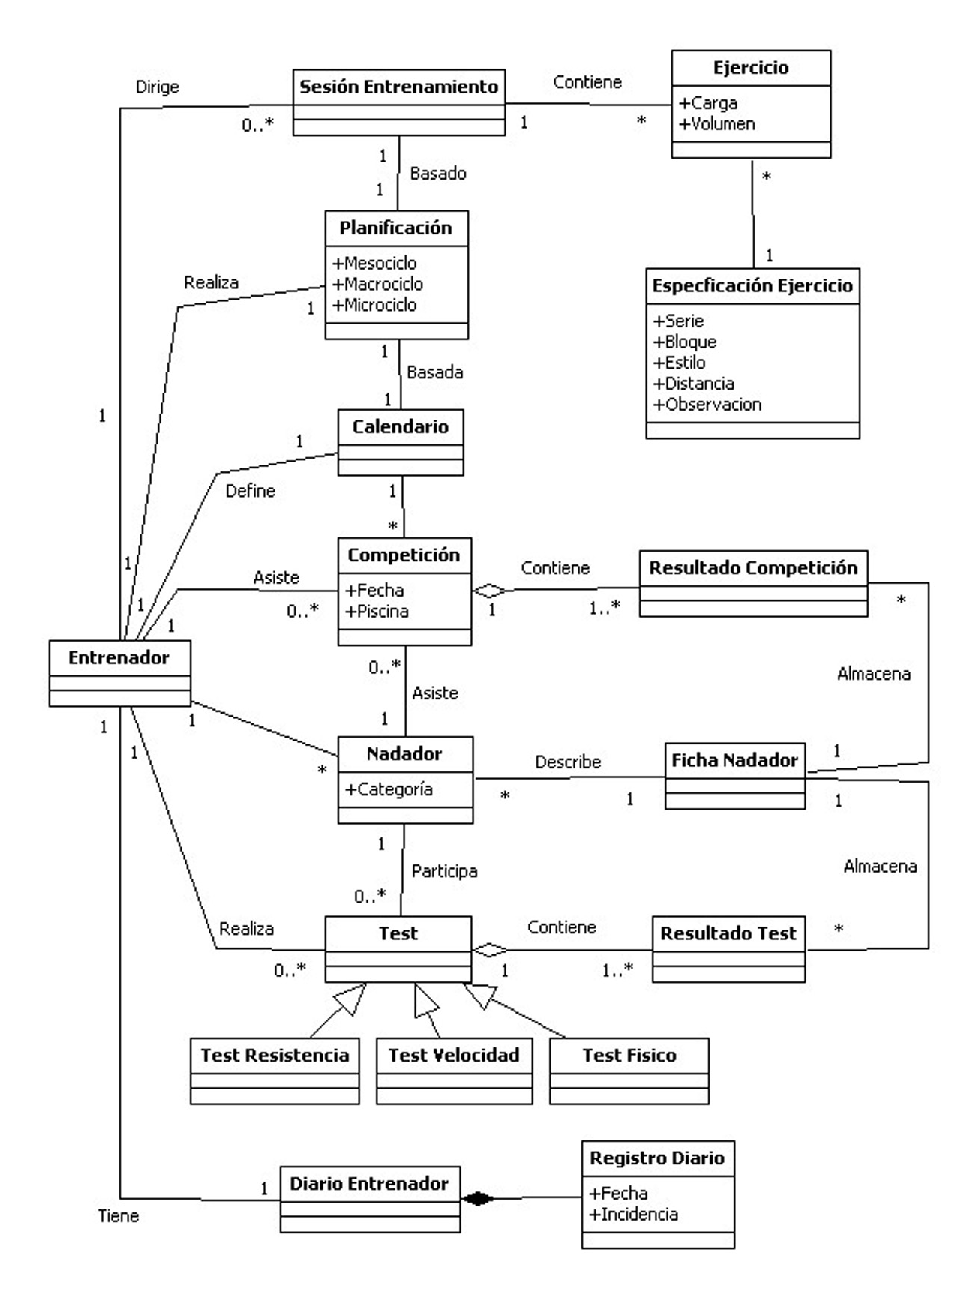
\includegraphics[width=400px]{./eps/captreq_modelo_dominio.eps}
	  \caption{Diagrama del modelo del dominio}
	  \label{fig:modelo_dominio}
	\end{figure}
	
	El recurso activo más importante en un equipo de natación son los nadadores. Los entrenadores dirigen grupos de nadadores agrupados por categorías, ayudando ello a que se puedan aplicar metodologías de entrenamientos a grupos homogéneos. Es cierto que, a pesar de que este sea el caso ideal, no siempre es posible. Hay veces en los que hay que agrupar a nadadores de diferentes edades para formar grupos. Los ejemplos más comunes que ocasionan esta situación son: la falta de espacio en las instalaciones donde se realizan las sesiones de entrenamientos o la falta de nadadores, debido a que es un equipo pequeño. Estas razones son las causantes de que en el modelo del dominio se exprese que un entrenador puede dirigir a cualquier nadador, independientemente de la categoría a la que pertenezca.
	
	Para controlar a cada nadador, el entrenador genera fichas que describen a cada uno de los nadadores. En ella se almacenan los datos personales, los datos de contacto y resultados obtenidos en test o competiciones. Sobre esto se hablará posteriormente.
	
	Al principio de una temporada y orientado a un grupo de nadadores, el cuerpo técnico realiza una planificación deportiva. El entrenador define un calendario con las competiciones a las cuales se asistirá, lo que conlleva que se marquen las pautas para definir los periodos de una planificación. Entiéndase por periodos la definición de macrociclos, mesociclos y microciclos.
	
	\begin{itemize}
		\item{{\bf Microciclo} es un conjunto de sesiones que tienen un objetivo concreto. Como su nombre indica, son ciclos breves de entrenamiento. Comúnmente, los microciclos hacen referencia a cada sesión de entrenamiento que realice un entrenador.}
		\item{{\bf Mesociclos} son bloques de microciclos {\bf ordenados} para conseguir un objetivo determinado: representan etapas relativamente acabas del proceso de entrenamiento que permiten asegurar el desarrollo de una capacidad.}
		\item{{\bf Macrociclo} es un bloque de mesociclos. La idea equivale al concepto de periodo de entrenamiento, los que normalmente suelen ir separados por reposos. } 
	\end{itemize}
	
	Uno de los fines de la planificación es obtener unos niveles de carga y volumen de cada microciclo, o lo que es lo mismo, especificar qué cantidad de metros y a qué intensidad se tienen que realizar cada una de las sesiones de entrenamientos. Es por ello, por lo que una sesión de entrenamiento contiene varios ejercicios de distinta tipología. Cada ejercicio refleja la capacidad que se trabaja, siendo los ejercicios aeróbicos \footnote{Aeróbicos incluyen cualquier tipo de ejercicio que se practique a niveles moderados de intensidad durante periodos de tiempo largos.}, anaeróbicos \footnote{Anaeróbicos comprenden actividades breves basadas en la fuerza.} y de técnica \footnote{La técnica hace referencia a la mejora de cada uno de los estilos de natación.} los más usuales.
	
	La especificación de cada ejercicio normalmente está compuesta por bloques, series, distancia, estilo que se nada y detalles más precisos que en el modelo se engloban como {\it observación}. Un ejemplo es {\it 2x(4x100 Mariposa) técnica variada}, el cuál expresa que se realicen 2 bloques de 4 series de 100 metros mariposa, haciendo ejercicios variados de distinta técnica. Esto sumaría un volumen total de 800 metros, generando una carga que se calcula a partir de un parámetro denominado {\it ``índice de Mujika''}.
	
	Por otro lado, otro de los fines de la planificación es preparar a los nadadores para las competiciones que se realicen y a las que se hayan decidido asistir. Por ello, se puede decir tanto entrenadores como nadadores asisten a alguna competición celebrada en una fecha y piscina determinada. Es importante reflejar la piscina, puesto que éstas pueden ser de 25 o 50 metros de longitud. Es lógico preguntarse, ¿en qué influye en el nadador la longitud de la piscina? Un nadador recorriendo una misma distancia en piscinas de 25 y de 50 metros, realiza un tiempo total distinto. 
	
	Dejando de lado una explicación técnica que explique el motivo, se puede afirmar que en una competición, un nadador puede realizar diferentes pruebas, lo que ocasionaría en una batería de resultados a almacenar en su ficha. El conjunto de todos los resultados de cada competición por cada nadador, forman la relación {\it Competición---Resultado competición}.
	
	Debido a que en el control está el éxito, para comprobar las capacidades de cada nadador, un entrenador realiza diferentes pruebas o {\it test}. Éstos pueden ser de diferente tipo, siendo los principales los que miden la resistencia, velocidad y otras capacidad físicas (tales como envergadura, talla o peso). Estas pruebas se realizan a lo largo de la temporada, obteniendo resultados que se almacenan también en la ficha del nadador.
	
	Por último, cada entrenador tiene un diario en el que registra las incidencias o sucesos que ocurren a lo largo de una temporada. Aporta información en una etapa de {\it feedback} \footnote{La realimentación, también denominada retroalimentación o feedback, significa ‘ida y vuelta’ y es, desde el punto de vista social y psicológico, el proceso de compartir observaciones, preocupaciones y sugerencias, con la intención de recabar información, a nivel individual o colectivo, para intentar mejorar el funcionamiento de una organización o de cualquier grupo formado por seres humanos.}, donde lo que importa es observar los sucesos del pasado para mejorar el proceso de entrenamiento (posibles cambios en el proceso de realización de planificación, ver como funciona un determinado ejercicio sobre una categoría o anotar competiciones a las que no ir en temporadas próximas son ejemplos de datos a añadir en el diario).    
	% -----------------------------------------------------------------------------
	%  NOTA: Añadir al modelo de dominio los tipos de ejercicios e índice e Mujika
	%	Corregir tilde de Especificación de Ejercicio -> observación
	% -----------------------------------------------------------------------------

	
% subsection construcción_del_modelo_del_dominio (end)

% section modelo_del_dominio (end)

% chapter captura_de_requisitos (end) % Captura de requisitos
	% ----------------------------------
% Cap Captura de Requisitos
% ----------------------------------
%

\chapter{Análisis} % (fold)
	\label{cha:analisis}

% 
% Sec Tipos de usuarios
%
\section{Casos de uso} % (fold)
	\label{sec:casos_de_uso}
	
	\begin{center}
		\begin{figure}
			\centering
			\caption{Diagrama de control de versiones distribuido}
			\label{fig:cvdistrib}
			\centering
		\end{figure}
	\end{center}
% section casos_de_uso (end)
% chapter análisis (end) % Especificacion de requisitos
	% ----------------------------------
% Cap Analisis
% ----------------------------------
\chapter{Análisis} % (fold)
	\label{cha:analisis}

	Durante el análisis, se analizan los requisitos que se describieron en la captura de requisitos, refinándolos y estructurándolos. El objetivo de hacerlo es conseguir una comprensión más precisa de los requisitos y una descripción de los mimos que sea fácil de mantener y que ayude a estructurar el sistema entero ---incluyendo su arquitectura.

	El lenguaje que se utiliza en el análisis se basa en un modelo de objetivos conceptual, llamado {\it modelo de análisis}. El modelo de análisis ayuda a refinar los requisitos y a razonar sobre los aspectos internos del sistema, incluidos sus recursos compartidos internos. De hecho, un recurso interno puede representarse como un objeto en el modelo de análisis. Además, el modelo de análisis ofrece un mayor poder expresivo y una mayor formalización, como por ejemplo, la que proporcionan los diagramas de interacción que se utilizan para describir los aspectos dinámicos del sistema.
	
	El modelo de análisis también nos ayuda a estructurar los requisitos como se ha explicado anteriormente y nos proporciona una estructura centrada en el mantenimiento, en aspectos tales como la flexibilidad ante los cambios y la reutilización. Esta estructura no sólo es útil para el mantenimiento de los requisitos como tales, sino que también se utiliza como entrada en las actividades de diseño e implementación. Se trata de preservar esta estructura a medida que se da forma al sistema. Por tanto, el modelo puede considerarse como una primera aproximación al modelo de diseño, aunque es un modelo por sí mismo. Mediante la conservación de la estructura del modelo de análisis durante el diseño, se obtiene un sistema que debería ser también mantenible como un todo: será flexible a los cambios en los requisitos, e incluirá elementos que podrán ser reutilizados cuando se construyan sistemas parecidos.
	
	Sin embargo, es importante hacer notar aquí que el modelo de análisis hace abstracciones, evitando resolver algunos problemas y tratar requisitos que pensamos que es mejor posponer al diseño y a la implementación. Debido a esto, no siempre se puede conservar la estructura proporcionada por el análisis, sino que se debe negociar y comprometer durante el diseño y la implementación. La razón por la cual esta <<conservación de la estructura>> no siempre tiene lugar en la práctica es sencillamente que el diseño debe considerar la plataforma de implementación: lenguaje de programación, sistemas operativos, entornos de trabajo, sistemas heredados y demás.
	
	\newpage
	
	\section{Diagramas de colaboración} % (fold)
		\label{sec:diagramas_de_colaboracion}
	
		Los diagramas de interacción son diagramas que describen cómo grupos de objetos colaboran para conseguir algún fin. Estos diagramas muestran objetos, así como los mensajes que se pasan entre ellos dentro del caso de uso, es decir, capturan el comportamiento de los casos de uso.
		
		Hay dos tipos de diagrama de interacción, ambos basados en la misma información, pero cada uno enfatizando un aspecto particular: Diagramas de Secuencia y {\bf Diagramas de Colaboración}.
		
		Un diagrama de colaboración, se puede decir que es una forma alternativa al diagrama de secuencias a la hora de mostrar un escenario. {\bf Este tipo de diagrama muestra las interacciones que ocurren entre los objetos que participan en una situación determinada.}
		
		En los diagramas de colaboración, se muestran las interacciones entre objetos creando enlaces entre ellos y añadiendo mensajes a esos enlaces. El nombre de un mensaje debería denotar el propósito del objeto invocante en la interacción con el objeto invocado.
		
		En este documento se detallan las principales colaboraciones relacionadas con los principales casos de uso descritos en el proyecto. Por tanto, se detallarán los diagramas de colaboración que hacen referencia a la {\it gestión de acceso, gestión del perfil, gestión de nadadores, gestión de los entrenamientos, gestión de competiciones, gestión test y diario de incidencia.}
		
		\subsection{Colaboraciones para la gestión del acceso} % (fold)
			\label{sub:colaboraciones_para_la_gestion_del_acceso}
		
		La primera de las colaboraciones es la referente al registro de entrenadores en el sistema ({\it véase} Figura \ref{fig:col_registrarse_entrenador}). Dado que es una aplicación distribuida para dar soporte a diferentes entrenadores, éstos tienen que formar parte del sistema  para posteriormente hacer uso de las funcionalidades. 
		
		Una vez que se finaliza el proceso de registro, el entrenador pasa a formar parte del conjunto de actores denominados {\it <<Entrenador Registrado>>}. 
		
			\begin{figure}[H]
			  \centering
			    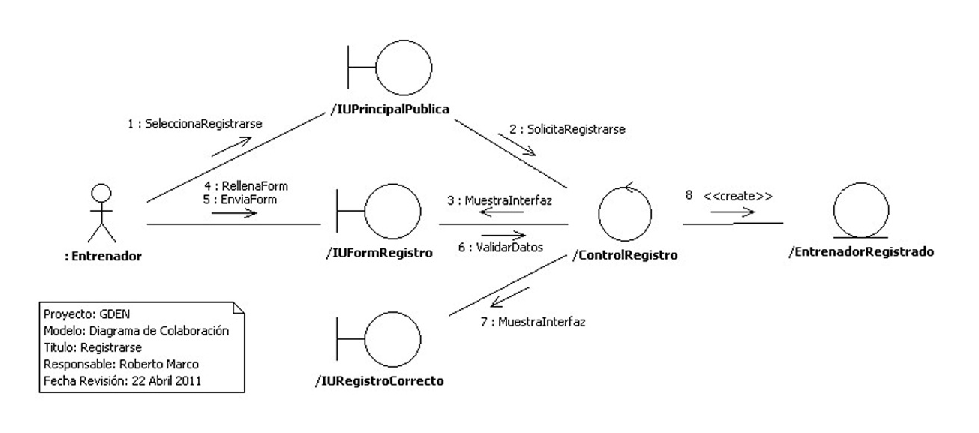
\includegraphics[width=16cm]{./eps/colaboraciones/gestion_acceso/RegistrarseEntrenador.eps}
			  \caption{Diagrama colaboración para registro de entrenador}
			  \label{fig:col_registrarse_entrenador}
			\end{figure}
			
		Seguido del proceso de registro, continúa el de identificación ({\it véase} Figura \ref{fig:col_identificarse_entrenador}) en la aplicación. El entrenador debe acceder al sistema con los datos que insertó en el formulario de registro. En caso de no ser así, fallará la validación. Si no hay ningún error, el controlador de sesión permitirá el inicio de sesión correctamente.
		
			\begin{figure}[H]
			  \centering
			    \includegraphics[width=16cm]{./eps/colaboraciones/gestion_acceso/IdentificarseEntrenador.eps}
			  \caption{Diagrama colaboración para identificación de entrenador}
			  \label{fig:col_identificarse_entrenador}
			\end{figure}
		
		% subsection colaboraciones_para_la_gestión_del_acceso (end)
	
		\subsection{Colaboraciones para la gestión del perfil} % (fold)
			\label{sub:colaboraciones_para_la_gestion_del_perfil}
			
		En la figura \ref{fig:col_cerrar_sesion_entrenador} se muestra el proceso para la finalización de una sesión previamente iniciada.
		
			\begin{figure}[H]
			  \centering
			    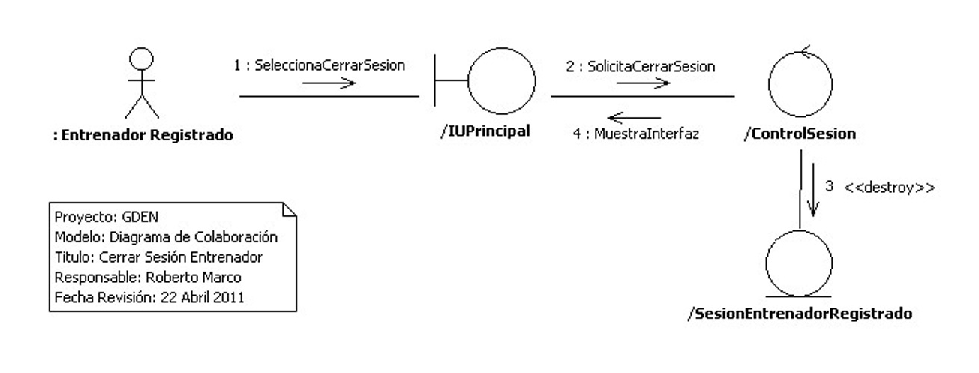
\includegraphics[width=16cm]{./eps/colaboraciones/gestion_perfil/CerrarSesionEntrenador.eps}
			  \caption{Diagrama colaboración para cerrar la sesión de entrenador}
			  \label{fig:col_cerrar_sesion_entrenador}
			\end{figure}
		
		Tras el registro e identificación, cada entrenador es poseedor de un perfil asociado. En él se almacenan los datos personales y de configuración de la sesión. Dada la naturaleza cambiante de la información, el entrenador puede modificar su perfil para actualizar sus datos ({\it véase} Figura \ref{fig:col_modificar_perfil} y \ref{fig:col_cambiar_contrasena}).
			
			\begin{figure}[H]
			  \centering
			    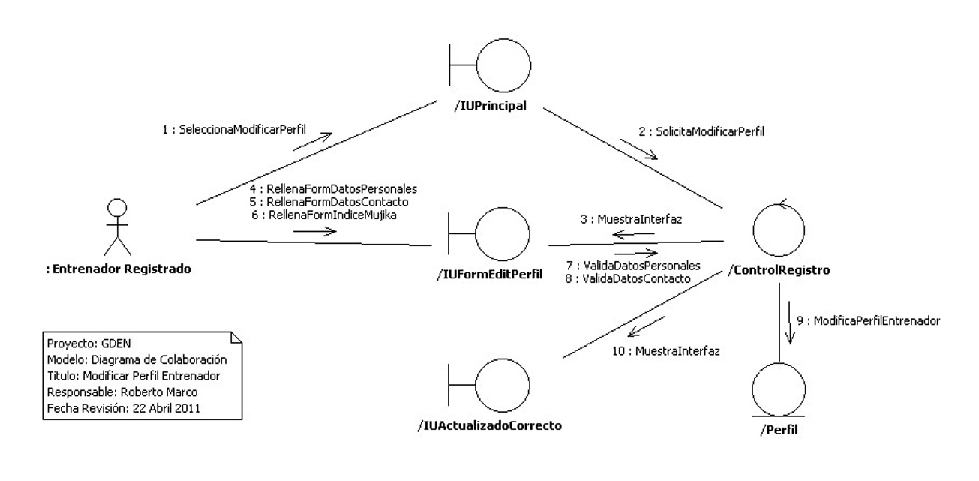
\includegraphics[width=16cm]{./eps/colaboraciones/gestion_perfil/ModificarPerfilEntrenador.eps}
			  \caption{Diagrama colaboración para modificar perfil del entrenador}
			  \label{fig:col_modificar_perfil}
			\end{figure}
			
			\begin{figure}[H]
			  \centering
			    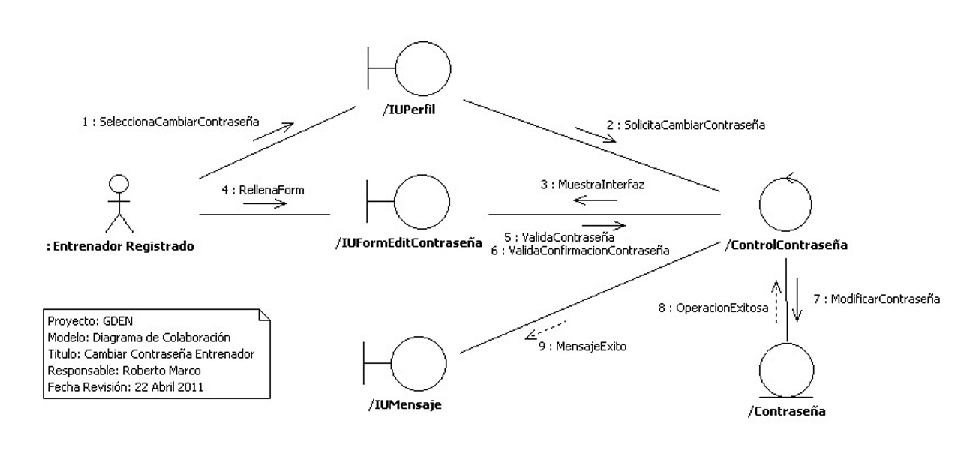
\includegraphics[width=16cm]{./eps/colaboraciones/gestion_perfil/CambiarContrasenaEntrenador.eps}
			  \caption{Diagrama colaboración para cambiar la contraseña del entrenador}
			  \label{fig:col_cambiar_contrasena}
			\end{figure}
		
		% subsection colaboraciones_para_la_gestión_del_perfil (end)
	
		\subsection{Colaboraciones para la gestión de nadadores} % (fold)
			\label{sub:colaboraciones_para_la_gestion_de_nadadores}
		
		La primera de las funcionalidades que se analizará será la de gestión de nadadores pertenecientes a un entrenador registrado. Se selecciona la opción de {\it añadir un nuevo nadador} y se rellenan los datos del formulario mostrado. En caso de éxito, se creará la entidad {\it nadador}.
		
			\begin{figure}[H]
			  \centering
			    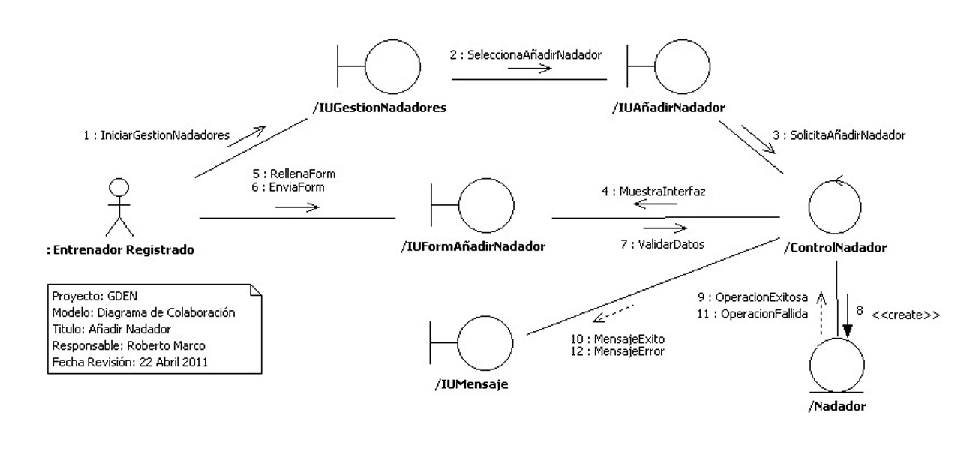
\includegraphics[width=16cm]{./eps/colaboraciones/gestion_nadadores/AnadirNadador.eps}
			  \caption{Diagrama colaboración para añadir nadador}
			  \label{fig:col_anadir_nadador}
			\end{figure}
		
		A medida que se van añadiendo nadadores al sistema, un entrenador está en disposición de ver un listado con los mismos ({\it véase} Figura \ref{fig:col_ver_lista_nadadores}). En la fase de diseño se puede determinar la forma en que se muestra el listado y la ordenación del mismo. De momento, el análisis es una fase más abstracta que no especifica más allá del cómo puede ser el proceso.
			
			\begin{figure}[H]
			  \centering
			    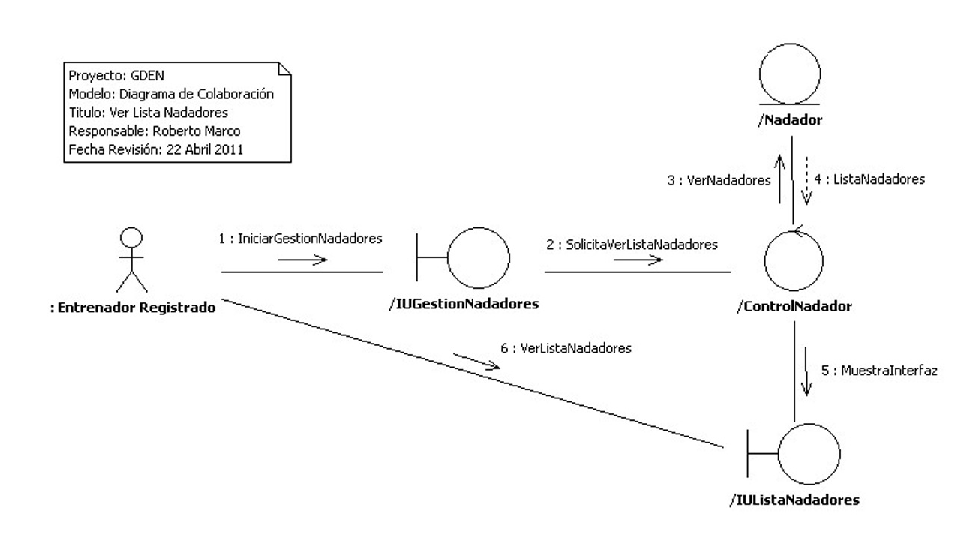
\includegraphics[width=16cm]{./eps/colaboraciones/gestion_nadadores/VerListaNadadores.eps}
			  \caption{Diagrama colaboración para ver lista nadadores}
			  \label{fig:col_ver_lista_nadadores}
			\end{figure}
			
		\newpage
			
			\begin{figure}[H]
			  \centering
			    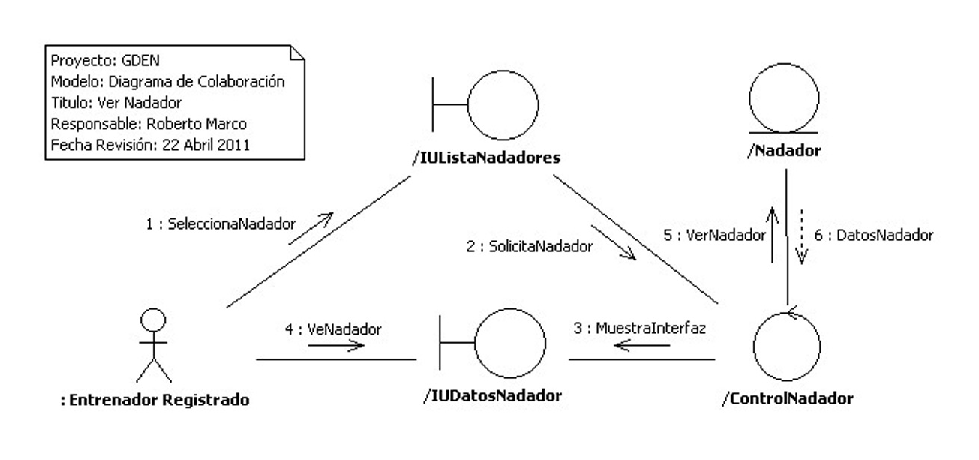
\includegraphics[width=16cm]{./eps/colaboraciones/gestion_nadadores/VerNadador.eps}
			  \caption{Diagrama colaboración para ver nadador}
			  \label{fig:col_ver_nadador}
			\end{figure}
			
		En la figura \ref{fig:col_ver_nadador} se muestra la colaboración para {\it ver un nadador}. El entrenador registrado solicita ver la ficha de un nadador determinado de la lista de nadadores totales. Esto es gestionado por el controlador, mostrando una interfaz con los datos pertinentes. A pesar de que no se refleje en el diagrama, los nadadores tienen resultados de competiciones y test asociados, por lo que se podría hacer una extensión del mismo accediendo a las entidades correspondientes.
		
			\begin{figure}[H]
			  \centering
			    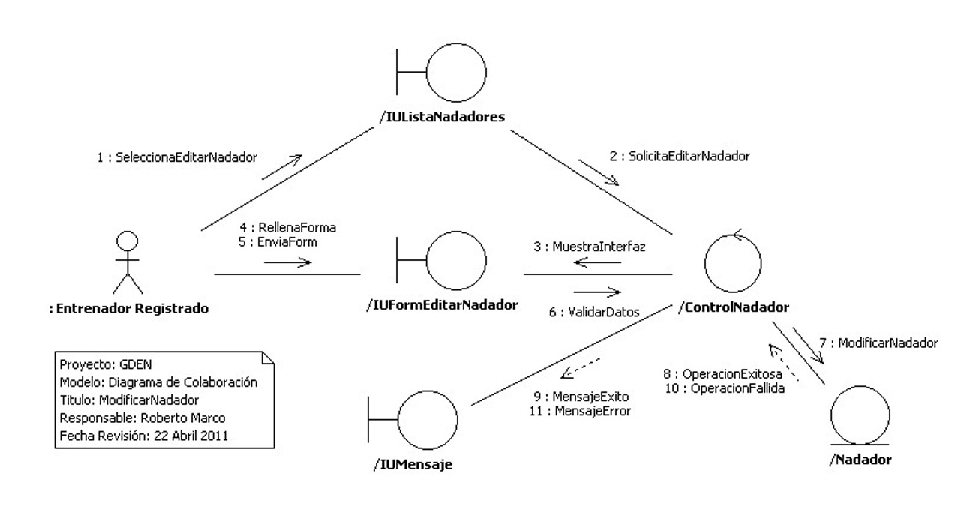
\includegraphics[width=16cm]{./eps/colaboraciones/gestion_nadadores/ModificarNadador.eps}
			  \caption{Diagrama colaboración para modificar nadador}
			  \label{fig:col_modificar_nadador}
			\end{figure}
			
			\begin{figure}[H]
			  \centering
			    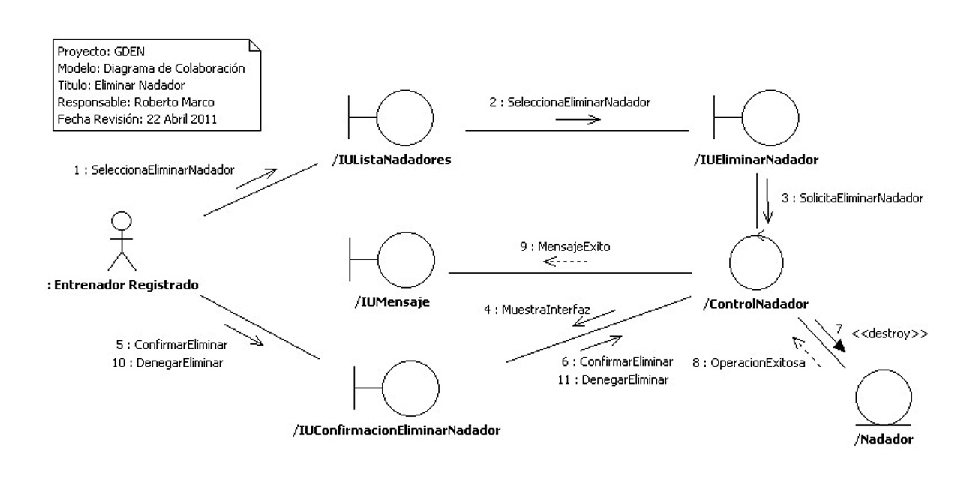
\includegraphics[width=16cm]{./eps/colaboraciones/gestion_nadadores/EliminarNadador.eps}
			  \caption{Diagrama colaboración para eliminar nadador}
			  \label{fig:col_eliminar_nadador}
			\end{figure}
		
		Tanto para la modificación como eliminación de un nadador ({\it véase} Figuras \ref{fig:col_modificar_nadador} y \ref{fig:col_eliminar_nadador}) el proceso es muy similar. La salvedad es que uno muestra un formulario editable para poder actualizar la información y el otro elimina un registro concreto perteneciente al entrenador registrado. Aunque en el diagrama no aparezca, en fases posteriores la colaboración tiene que ser extendida para poder eliminar los registros de resultados de competiciones y test asociados a un nadador.
		
		Para el resto de colaboraciones únicamente se mostrarán los diagramas debido a que los procesos son muy parecidos.
			
		% subsection colaboraciones_para_la_gestión_de_nadadores (end)
		
		\subsection{Colaboraciones para la gestión de entrenamientos} % (fold)
			\label{sub:colaboraciones_para_la_gestion_de_entrenamientos}
		
			\begin{figure}[H]
			  \centering
			    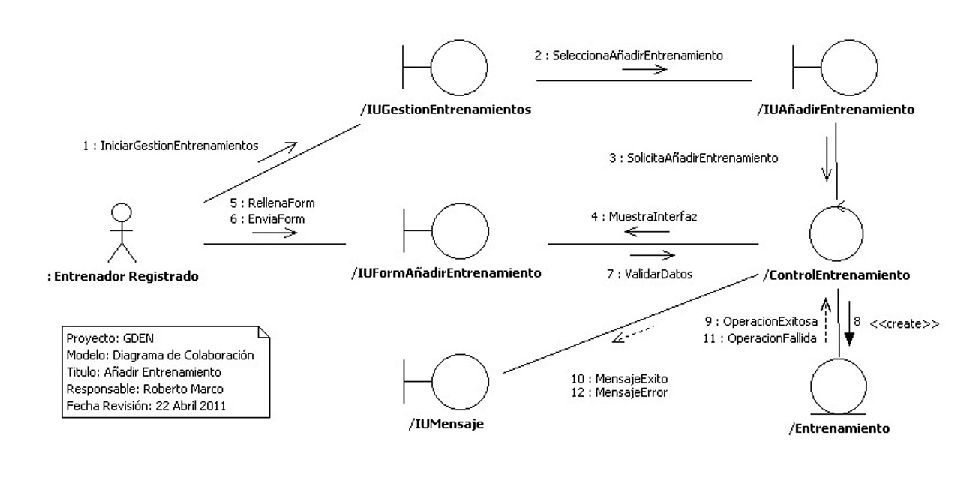
\includegraphics[width=16cm]{./eps/colaboraciones/gestion_entrenamiento/AnadirEntrenamiento.eps}
			  \caption{Diagrama colaboración para añadir entrenamiento}
			  \label{fig:col_anadir_entrenamiento}
			\end{figure}
			
			\begin{figure}[H]
			  \centering
			    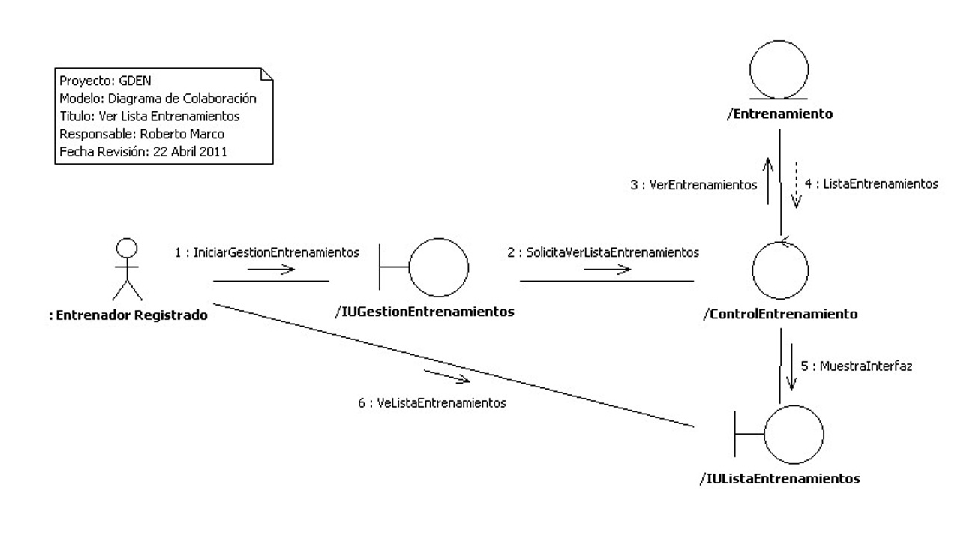
\includegraphics[width=16cm]{./eps/colaboraciones/gestion_entrenamiento/VerListaEntrenamientos.eps}
			  \caption{Diagrama colaboración para ver lista de entrenamientos}
			  \label{fig:col_ver_lista_entrenamientos}
			\end{figure}
			
			\begin{figure}[H]
			  \centering
			    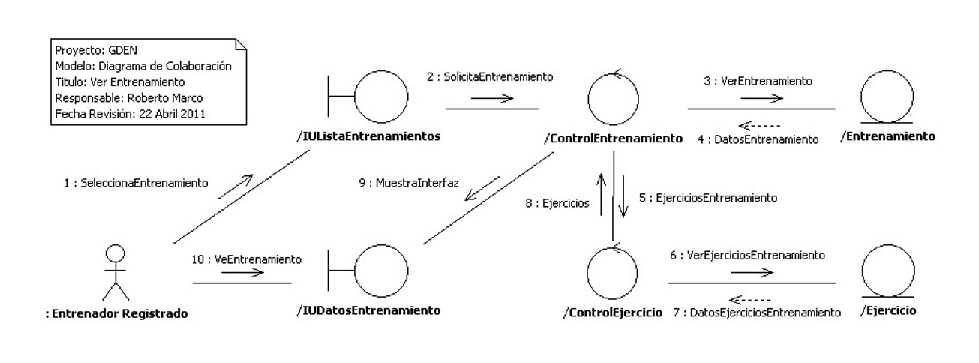
\includegraphics[width=16cm]{./eps/colaboraciones/gestion_entrenamiento/VerEntrenamiento.eps}
			  \caption{Diagrama colaboración para ver entrenamiento}
			  \label{fig:col_ver_entrenamiento}
			\end{figure}
			
			\begin{figure}[H]
			  \centering
			    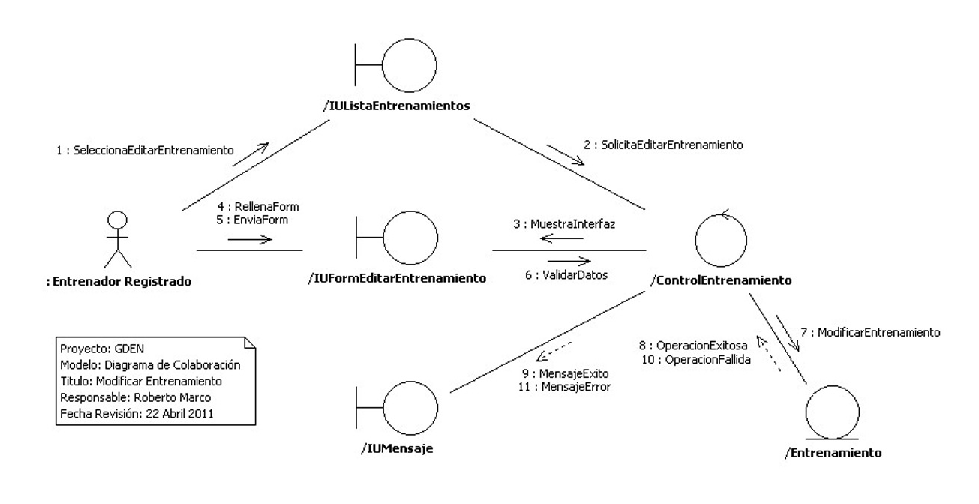
\includegraphics[width=16cm]{./eps/colaboraciones/gestion_entrenamiento/ModificarEntrenamiento.eps}
			  \caption{Diagrama colaboración para modificar entrenamiento}
			  \label{fig:col_modificar_entrenamiento}
			\end{figure}
			
			\begin{figure}[H]
			  \centering
			    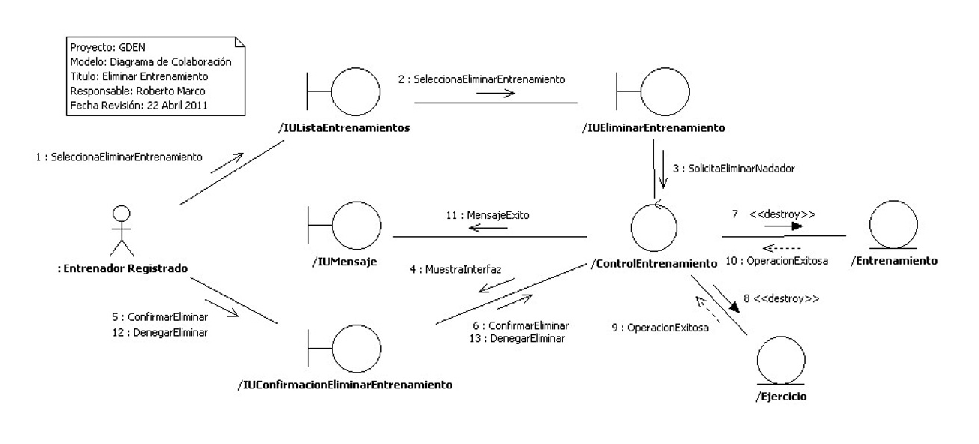
\includegraphics[width=16cm]{./eps/colaboraciones/gestion_entrenamiento/EliminarEntrenamiento.eps}
			  \caption{Diagrama colaboración para eliminar entrenamiento}
			  \label{fig:col_eliminar_entrenamiento}
			\end{figure}
		% subsection colaboraciones_para_la_gestión_de_entrenamientos (end)
	
		\subsection{Colaboraciones para la gestión de competiciones} % (fold)
			\label{sub:colaboraciones_para_la_gestion_de_competiciones}
		
			\begin{figure}[H]
			  \centering
			    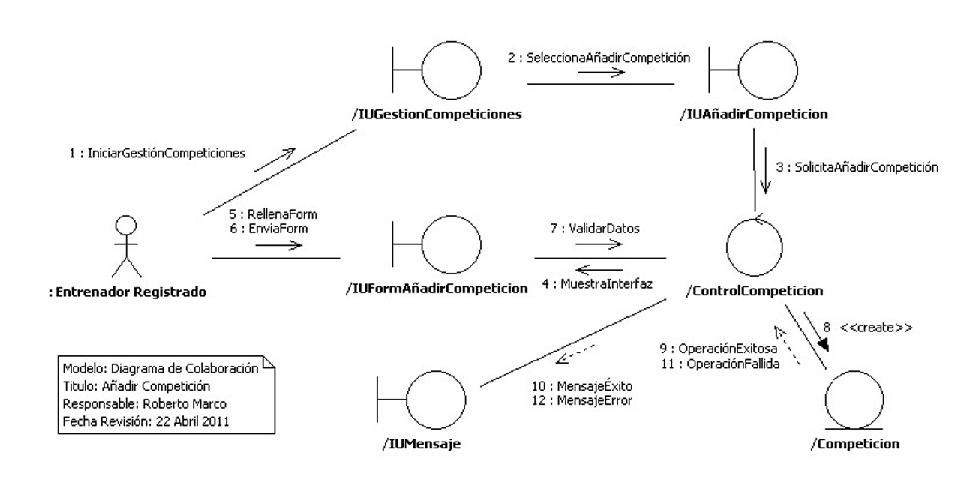
\includegraphics[width=16cm]{./eps/colaboraciones/gestion_competiciones/AnadirCompeticion.eps}
			  \caption{Diagrama colaboración para añadir competición}
			  \label{fig:col_anadir_competicion}
			\end{figure}
			
			\begin{figure}[H]
			  \centering
			    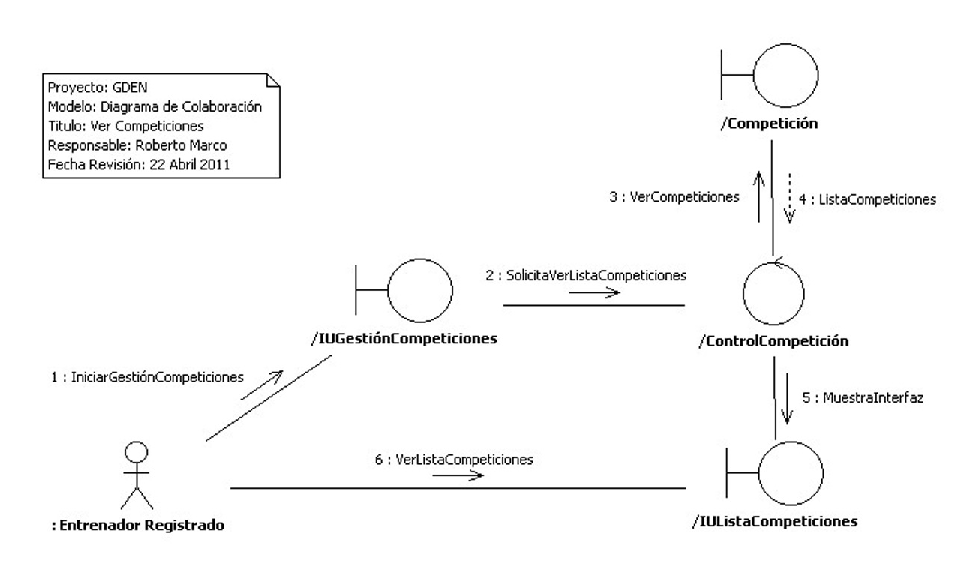
\includegraphics[width=16cm]{./eps/colaboraciones/gestion_competiciones/VerListaCompeticiones.eps}
			  \caption{Diagrama colaboración para ver lista de competiciones}
			  \label{fig:col_ver_lista_competiciones}
			\end{figure}
			
			\begin{figure}[H]
			  \centering
			    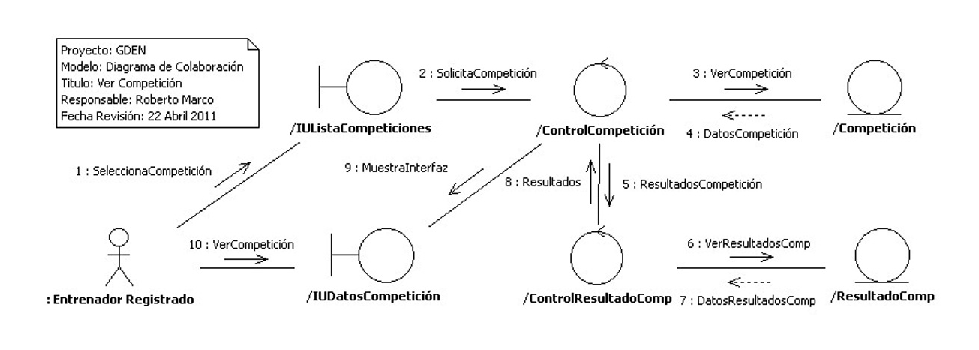
\includegraphics[width=16cm]{./eps/colaboraciones/gestion_competiciones/VerCompeticion.eps}
			  \caption{Diagrama colaboración para ver competición}
			  \label{fig:col_ver_competicion}
			\end{figure}
			
			\begin{figure}[H]
			  \centering
			    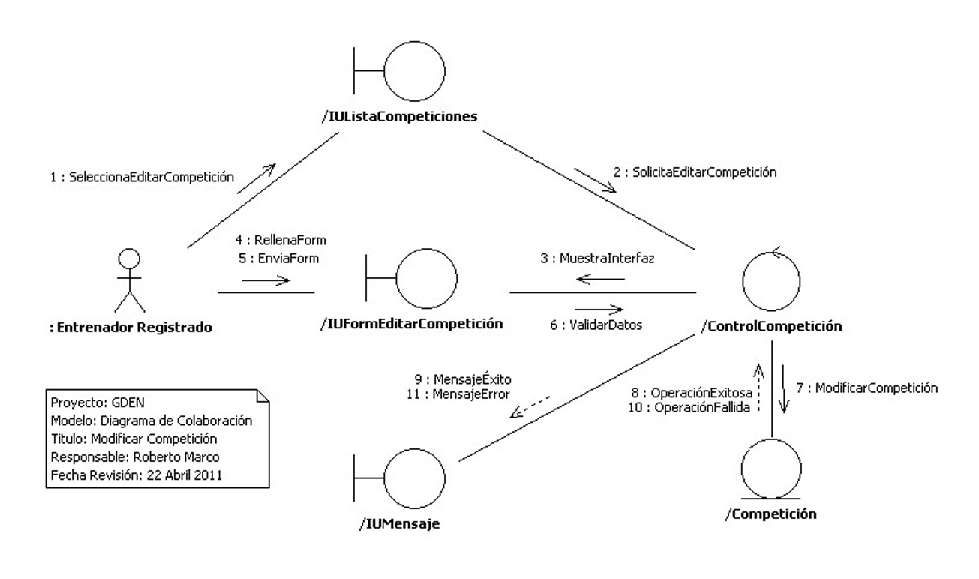
\includegraphics[width=16cm]{./eps/colaboraciones/gestion_competiciones/ModificarCompeticion.eps}
			  \caption{Diagrama colaboración para modificar competición}
			  \label{fig:col_modificar_competicion}
			\end{figure}
			
			\begin{figure}[H]
			  \centering
			    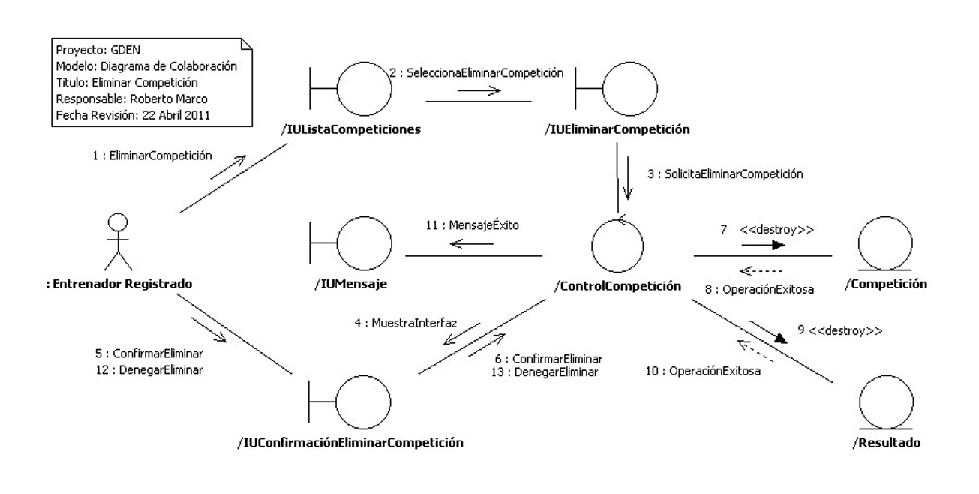
\includegraphics[width=16cm]{./eps/colaboraciones/gestion_competiciones/EliminarCompeticion.eps}
			  \caption{Diagrama colaboración para eliminar competición}
			  \label{fig:col_eliminar_competicion}
			\end{figure}
			
		% subsection colaboraciones_para_la_gestión_de_competiciones (end)
		
		\subsection{Colaboraciones para la gestión de test} % (fold)
			\label{sub:colaboraciones_para_la_gestion_de_test}
			
			\begin{figure}[H]
			  \centering
			    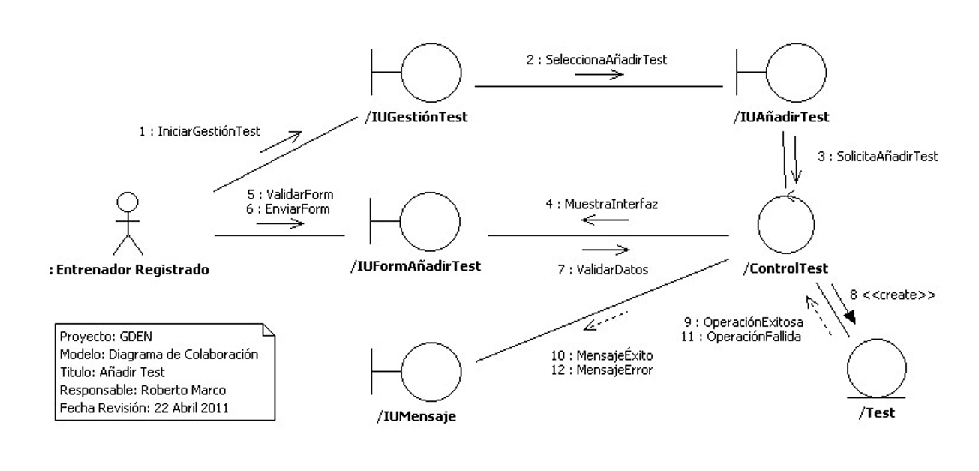
\includegraphics[width=16cm]{./eps/colaboraciones/gestion_test/AnadirTest.eps}
			  \caption{Diagrama colaboración para añadir test}
			  \label{fig:col_anadir_test}
			\end{figure}
			
			\begin{figure}[H]
			  \centering
			    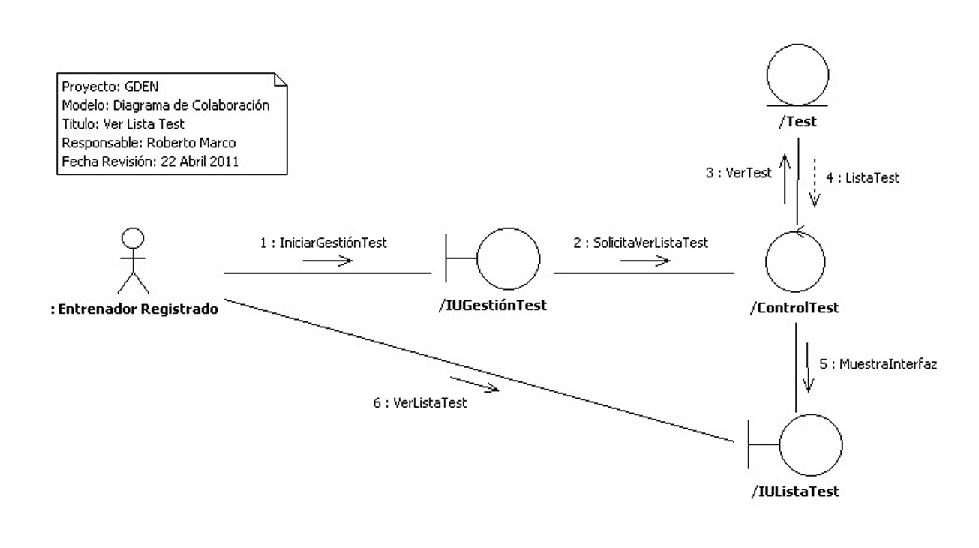
\includegraphics[width=16cm]{./eps/colaboraciones/gestion_test/VerListaTest.eps}
			  \caption{Diagrama colaboración para ver lista test}
			  \label{fig:col_ver_lista_test}
			\end{figure}
			
			\begin{figure}[H]
			  \centering
			    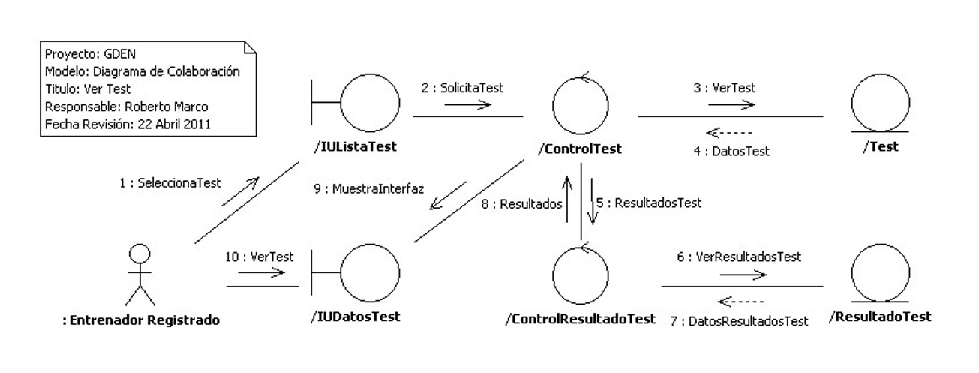
\includegraphics[width=16cm]{./eps/colaboraciones/gestion_test/VerTest.eps}
			  \caption{Diagrama colaboración para ver test}
			  \label{fig:col_ver_test}
			\end{figure}
			
			\begin{figure}[H]
			  \centering
			    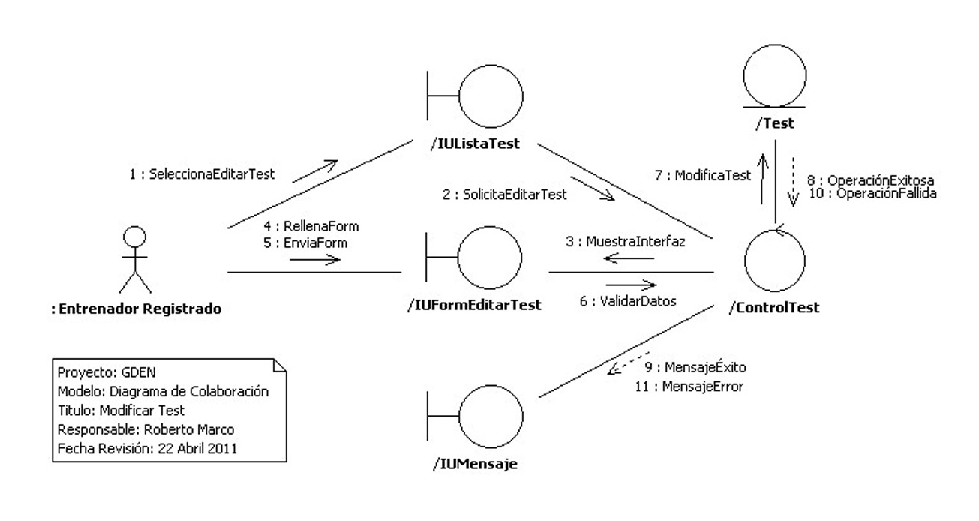
\includegraphics[width=16cm]{./eps/colaboraciones/gestion_test/ModificarTest.eps}
			  \caption{Diagrama colaboración para modificar test}
			  \label{fig:col_modificar_test}
			\end{figure}
			
			\begin{figure}[H]
			  \centering
			    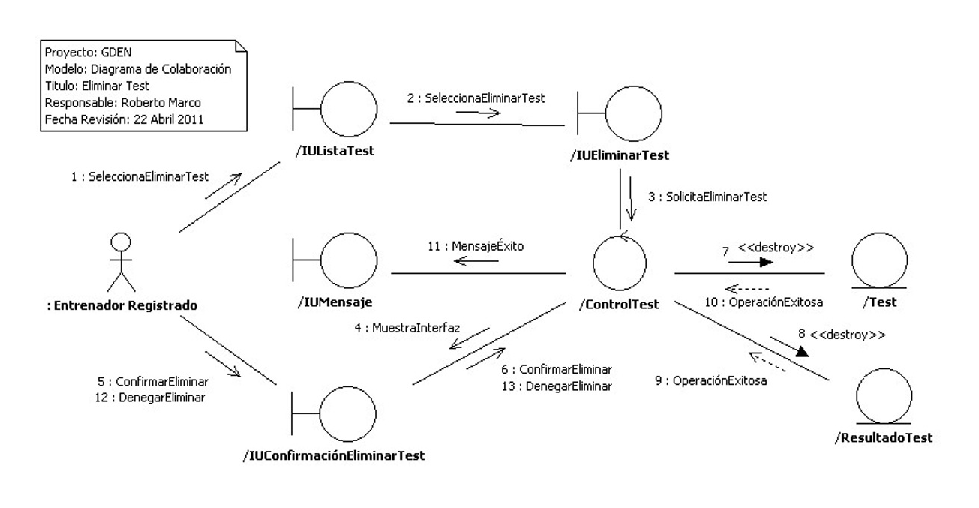
\includegraphics[width=16cm]{./eps/colaboraciones/gestion_test/EliminarTest.eps}
			  \caption{Diagrama colaboración para eliminar test}
			  \label{fig:col_eliminar_test}
			\end{figure}
		
		% subsection colaboraciones_para_la_gestión_de_test (end)
		
		\subsection{Colaboraciones para la gestión del diario de incidencias} % (fold)
			\label{sub:colaboraciones_para_la_gestion_del_diario_de_incidencias}
			
			\begin{figure}[H]
			  \centering
			    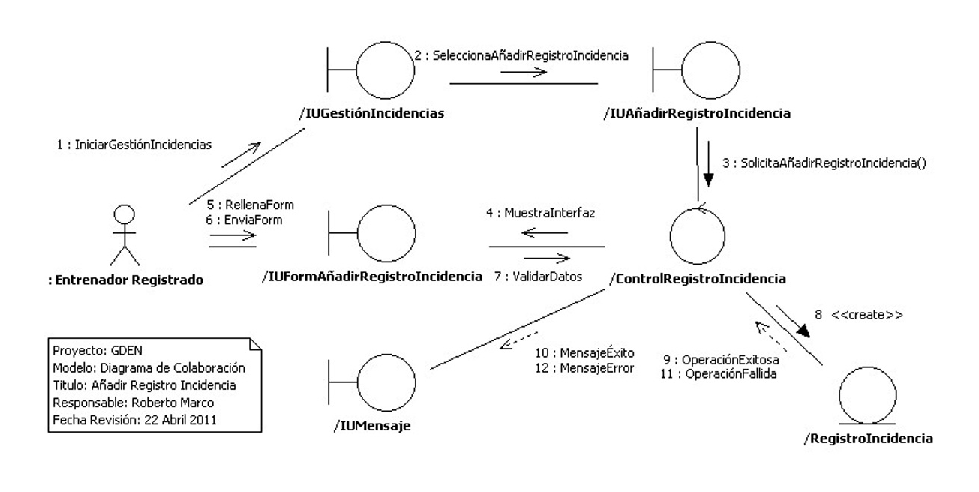
\includegraphics[width=16cm]{./eps/colaboraciones/gestion_diarioincidencia/AnadirRegistroIncidencia.eps}
			  \caption{Diagrama colaboración para añadir incidencia}
			  \label{fig:col_anadir_incidencia}
			\end{figure}
			
			\begin{figure}[H]
			  \centering
			    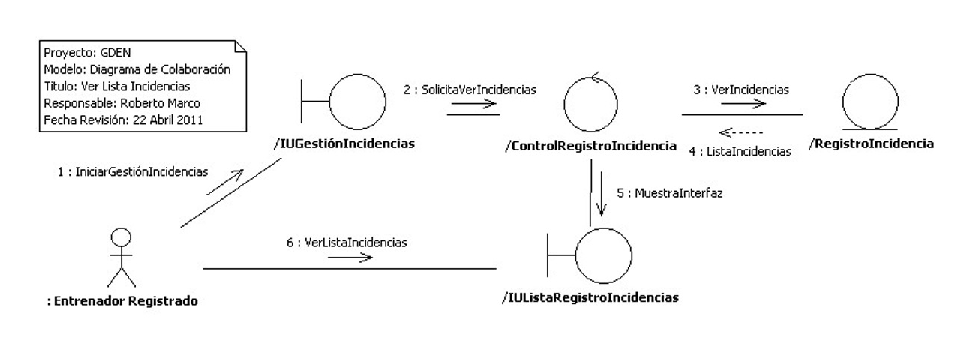
\includegraphics[width=16cm]{./eps/colaboraciones/gestion_diarioincidencia/VerListaRegistroIncidencias.eps}
			  \caption{Diagrama colaboración para ver lista de incidencias}
			  \label{fig:col_ver_lista_incidencias}
			\end{figure}
			
			\begin{figure}[H]
			  \centering
			    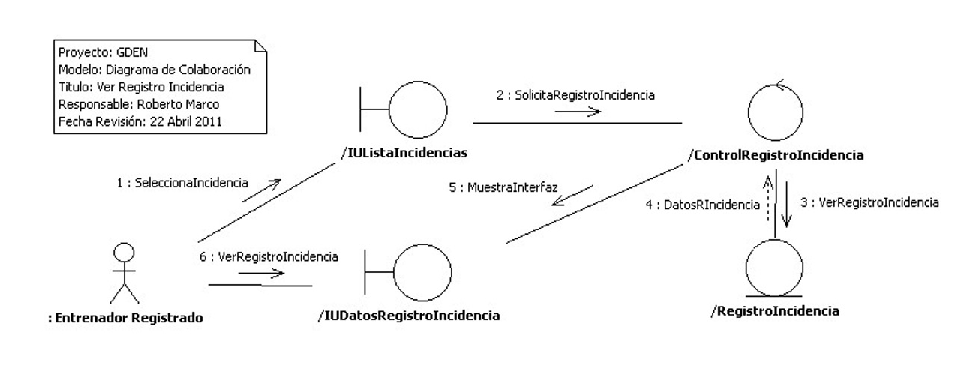
\includegraphics[width=16cm]{./eps/colaboraciones/gestion_diarioincidencia/VerRegistroIncidencia.eps}
			  \caption{Diagrama colaboración para ver incidencia}
			  \label{fig:col_ver_incidencia}
			\end{figure}
			
			\begin{figure}[H]
			  \centering
			    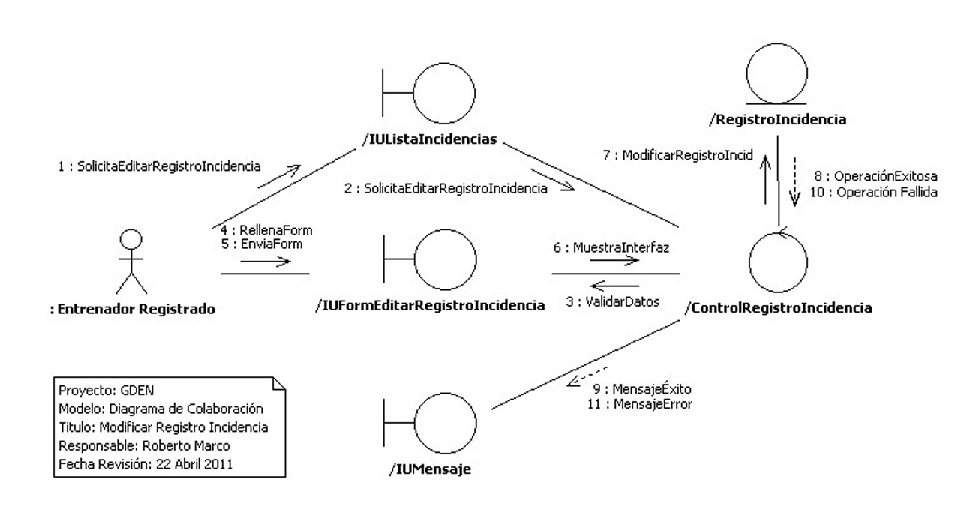
\includegraphics[width=16cm]{./eps/colaboraciones/gestion_diarioincidencia/ModificarRegistroIncidencia.eps}
			  \caption{Diagrama colaboración para modificar incidencia}
			  \label{fig:col_modificar_incidencia}
			\end{figure}
			
			\begin{figure}[H]
			  \centering
			    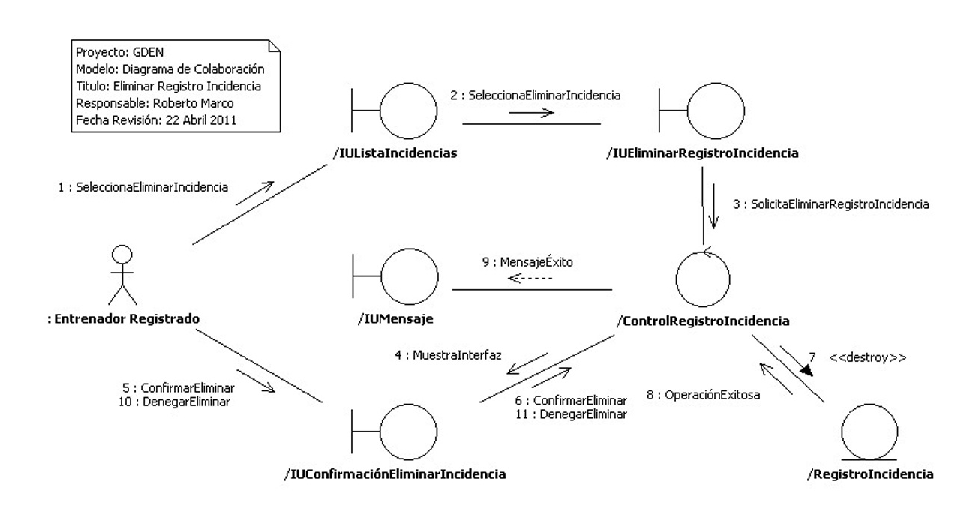
\includegraphics[width=16cm]{./eps/colaboraciones/gestion_diarioincidencia/EliminarRegistroIncidencia.eps}
			  \caption{Diagrama colaboración para eliminar incidencia}
			  \label{fig:col_eliminar_incidencia}
			\end{figure}
		% subsection colaboraciones_para_la_gestión_del_diario_de_incidencias (end)
	% section diagramas_de_colaboración (end)
		
	\section{Diagrama de clases} % (fold)
		\label{sec:diagrama_de_clases}
		
		Los autores Jacobson, Booch y Rumbaugh definen en la guía del proceso unificado de desarrollo de software \cite{PUJac08} una clase de análisis como: {\it <<una abstracción de una o varias clases y/o subsistemas del diseño del sistema>>}. Esta abstracción posee las siguientes características:
		
		\begin{itemize}
			\item Una clase de análisis se centra en el tratamiento de los requisitos funcionales y pospone los no funcionales.
			\item Esto hace que una clase de análisis sea más evidente en el contexto del dominio del problema, a menudo de mayor granularidad que sus contrapartidas de diseño e implementación.
			\item Una clase de análisis raramente define u ofrece un interfaz en términos de operaciones y de sus signaturas. Sin embargo, su comportamiento se define mediante responsabilidades en un nivel más alto y menos formal.
			\item Una clase de análisis define atributos, aunque esos atributos también son de un nivel bastante alto.
			\item Una clase de análisis participa en relaciones, aunque esas relaciones son más conceptuales que sus contrapartidas de diseño e implementación.
			\item Las clases de análisis siempre encajan en uno de tres estereotipos básicos: de interfaz, de control o de entidad.
		\end{itemize}
		
		\subsection{Nadadores} % (fold)
			\label{sub:nadadores}
		
			\begin{figure}[H]
			  \centering
			    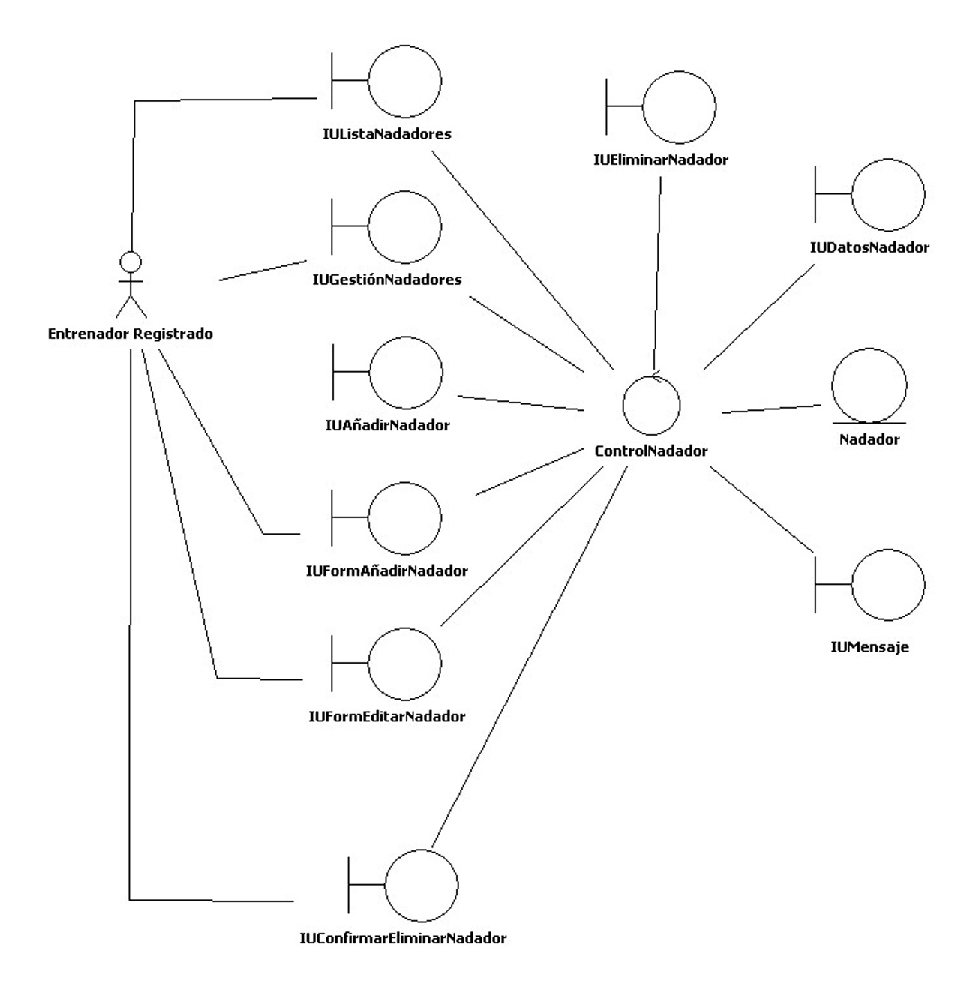
\includegraphics[width=14cm]{./eps/an_diagclases/GestionNadadores.eps}
			  \caption{Diagrama de clases Nadadores}
			  \label{fig:an_diagclases_nadadores}
			\end{figure}
			
		% subsection nadadores (end)
	
		\subsection{Competiciones} % (fold)
			\label{sub:competiciones}
		
			\begin{figure}[H]
			  \centering
			    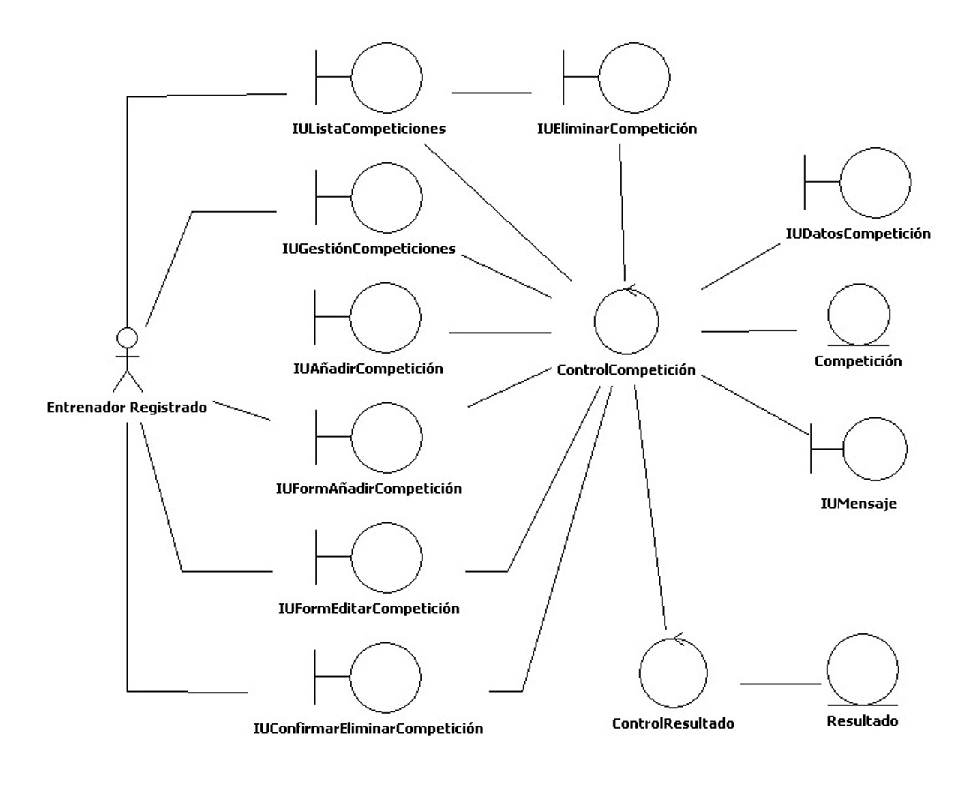
\includegraphics[width=14cm]{./eps/an_diagclases/GestionCompeticiones.eps}
			  \caption{Diagrama de clases Competiciones}
			  \label{fig:an_diagclases_competiciones}
			\end{figure}
		% subsection competiciones (end)
		
		\subsection{Entrenamientos} % (fold)
			\label{sub:entrenamientos}
			
			\begin{figure}[H]
			  \centering
			    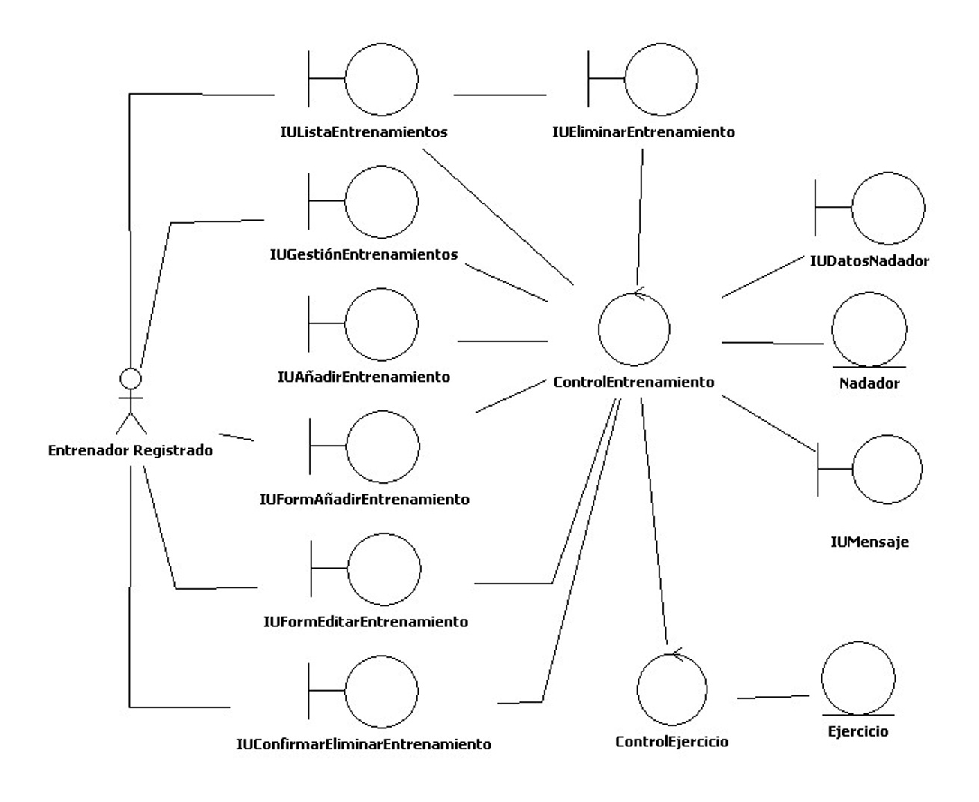
\includegraphics[width=14cm]{./eps/an_diagclases/GestionEntrenamientos.eps}
			  \caption{Diagrama de clases Entrenamientos}
			  \label{fig:an_diagclases_entrenamientos}
			\end{figure}
		% subsection entrenamientos (end)
		
		\subsection{Test} % (fold)
			\label{sub:test}
			
			\begin{figure}[H]
			  \centering
			    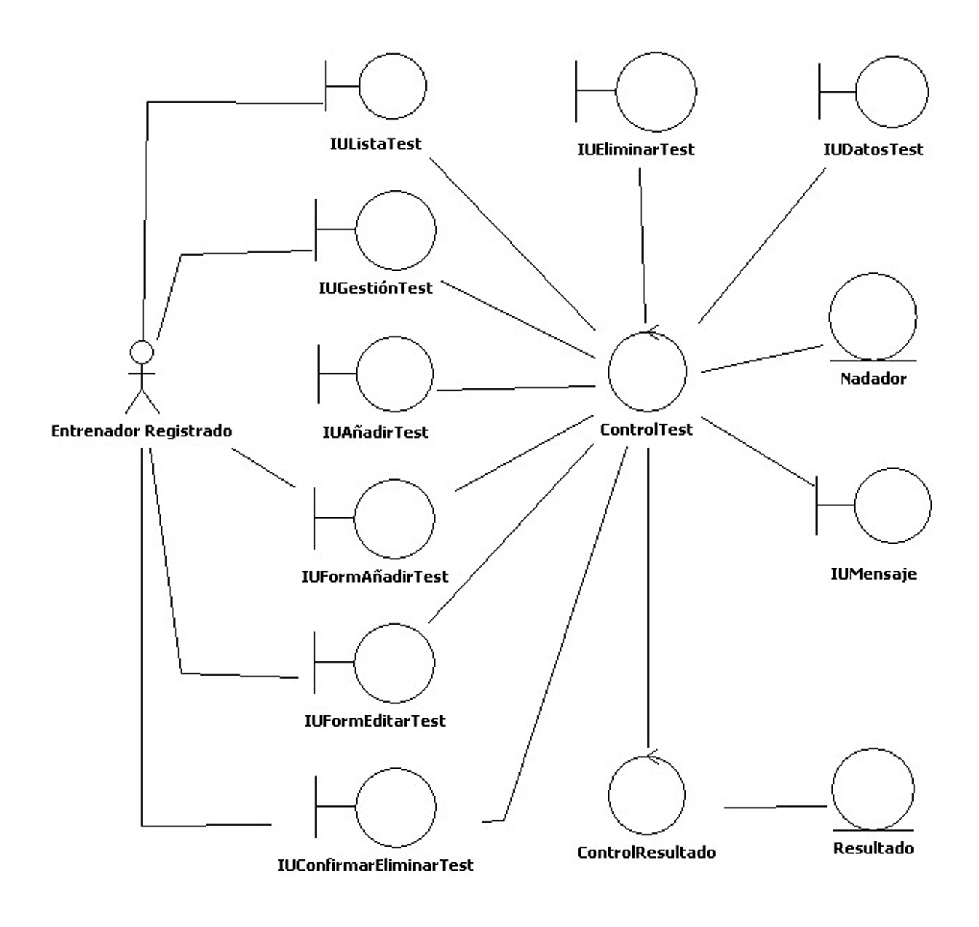
\includegraphics[width=14cm]{./eps/an_diagclases/GestionTest.eps}
			  \caption{Diagrama de clases Test}
			  \label{fig:an_diagclases_test}
			\end{figure}
		% subsection test (end)
		
		\subsection{Diario de Incidencias} % (fold)
			\label{sub:diario_de_incidencias}
			
			\begin{figure}[H]
			  \centering
			    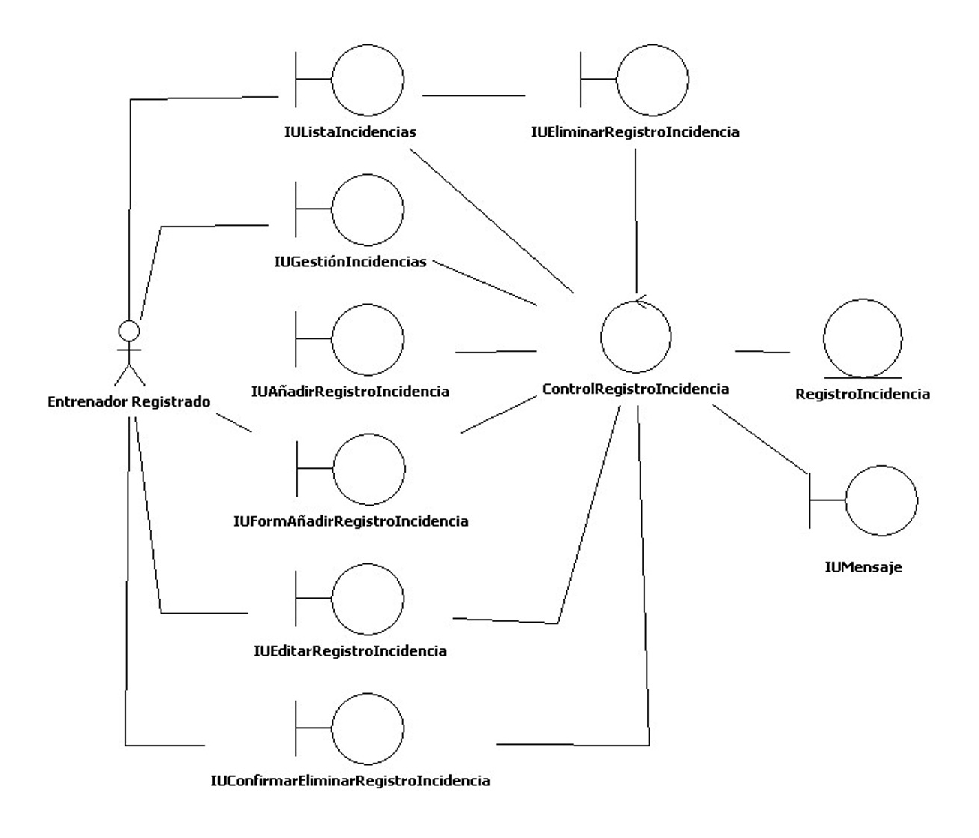
\includegraphics[width=14cm]{./eps/an_diagclases/GestionIncidencias.eps}
			  \caption{Diagrama de clases Incidencias}
			  \label{fig:an_diagclases_incidencias}
			\end{figure}
		% subsection diario_de_incidencias (end)
	% section diagrama_de_clases (end)	
	
	\section{Diagrama de paquetes} % (fold)
		\label{sec:diagrama_de_paquetes_analisis}
		
		Es la metodología del proceso unificado, es el arquitecto de software quien realiza un {\bf análisis de la arquitectura}. El propósito de este análisis es esbozar el modelo de análisis y la arquitectura mediante la identificación de paquetes del análisis, clases del análisis evidentes y requisitos especiales comunes.
		
		Los {\bf paquetes del análisis} proporcionan un medio para organizar el modelo de análisis en piezas más pequeñas y más manejables. Puede, bien identificarse inicialmente como forma de dividir el trabajo de análisis, o bien encontrase a medida que el modelo de análisis evoluciona y <<crece>>, convirtiéndose en una gran estructura que debe descomponerse.
		
		Una identificación inicial de los paquetes del análisis se hace de manera natural basándonos en los requisitos funcionales y en el dominio del problema, es decir, en la aplicación que estamos considerando. Debido a que capturamos los requisitos funcionales en la forma de casos de uso, una forma directa de identificar paquetes del análisis es asignar la mayor parte de un cierto número de casos de uso a un paquete concreto y, posteriormente, realizar la funcionalidad correspondiente dentro de ese paquete. Entre las <<asignaciones>> adecuadas de casos de uso a un paquete en concreto se tienen las siguientes:
		\begin{itemize}
			\item Los casos de uso requeridos para dar soporte a un determinado proceso de negocio.
			\item Los casos de uso requeridos para dar soporte a un determinado actor del sistema.
			\item Los casos de uso que están relacionados mediante relaciones de generalización y de extensión.
		\end{itemize}
		
		La arquitectura del sistema estará dividida en diferentes capas: {\it capa específica, capa genérica, capa middleware o entorno de trabajo y capa del sistema operativo}. En el análisis se dará forma a las dos primeras, lo que ayudará a tener una base para la fase de diseño.
		
		\begin{figure}[H]
		  \centering
		    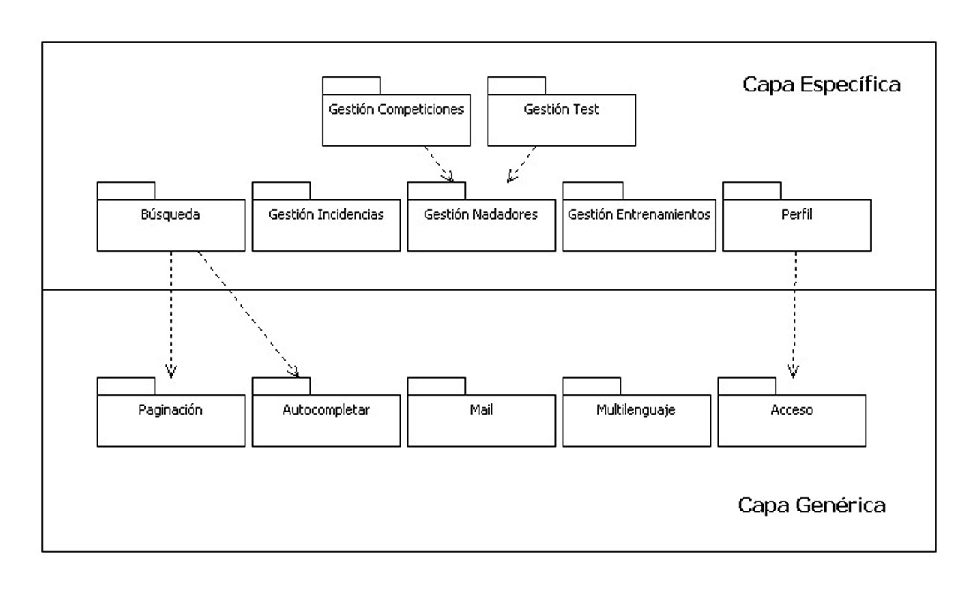
\includegraphics[width=14cm]{./eps/an_diagpaquetes/an_diagpaquetes.eps}
		  \caption{Diagrama de paquetes para el análisis}
		  \label{fig:an_diagpaquetes}
		\end{figure}
		
		En la figura \ref{fig:an_diagpaquetes} se muestran los principales paquetes que se detectan en la aplicación para las capas genérica y específica. Siguen la misma estructura de descomposición del modelo de casos de uso, donde cada uno de los paquetes da soporte a un proceso del negocio.
	% section diagrama_de_paquetes (end)

% chapter analisis (end) % Analisis
	% ----------------------------------
% Cap Diseño
% ----------------------------------
\chapter{Diseño} % (fold)
	\label{cha:diseno}
	
	En el diseño se modela el sistema y se encuentra su forma (incluida la arquitectura) para que soporte todos los requisitos ---incluyendo los requisitos no funcionales y otras restricciones--- que se le suponen. Una entrada esencial en el diseño es el resultado del análisis, esto es, el modelo del análisis (véase capítulo \ref{cha:analisis}). El modelo de análisis proporciona una comprensión detallada de los requisitos. Y lo que es más importante, impone una estructura del sistema que debemos esforzarnos por conservar lo más fielmente posible cuando demos forma al sistema. En concreto, los propósitos del diseño son:
	\begin{itemize}
		\item Adquirir una comprensión en profundidad de los aspectos relacionados con los requisitos no funcionales y restricciones relacionadas con los lenguajes de programación, componentes reutilizables, sistemas operativos, tecnologías de distribución, tecnologías de interfaz de usuario, etc.
		\item Crear un entrada apropiada y un punto de partida para actividades de implementación subsiguientes capturando los requisitos o subsistemas individuales, interfaces y clases.
		\item Ser capaces de descomponer los trabajos de implementación en partes más manejables que puedan ser llevadas a cabo por diferentes equipos de desarrollo, teniendo en cuenta la posible concurrencia. Esto resulta útil en los casos en los que la descomposición no pueda ser hecha basándose en los resultados de la captura de requisitos o análisis. 
		\item Ser capaces de visualizar y reflexionar sobre el diseño utilizando una notación común.
		\item Crear una abstracción sin costuras de la implementación del sistema, en el sentido de que la implementación es un refinamiento directo del diseño que rellena lo existente sin cambiar la estructura. 
	\end{itemize}
	
	%
  % Sec Prototipo de interfaz de usuario
  %
  \section{Prototipo de interfaz de usuario} % (fold)
  	\label{sec:prototipo_de_interfaz_de_usuario}

    Para situar al lector de la idea que se tiene sobre el software a desarrollar, se comenzará la fase de diseño exponiendo los prototipos desarrollados.
    
  	\subsection{Introducción} % (fold)
  		\label{sub:analisis_prototipo_introduccion}

  		El paradigma de creación de prototipos puede ser cerrado o abierto. El enfoque cerrado se denomina {\it prototipo desechable.} Este prototipo sirve únicamente como una basta demostración de los requisitos. Después se desecha y se hace una ingeniería del software con un paradigma diferente. Un enfoque abierto, denominado {\it prototipo evolutivo}, emplea el prototipo como primera parte de una actividad de análisis a la que seguirá el diseño y la construcción. 

  		Antes de poder elegir un enfoque abierto o cerrado, es necesario determinar si se puede crear un prototipo del sistema a construir. Se pueden definir varios favores candidatos a la creación de prototipos \cite{BOA84}: área de aplicación, complejidad, características del cliente y del proyecto.

  		En general, cualquier aplicación que cree pantallas visuales dinámicas, interactúe intensamente con el ser humano, o demande de algoritmos o procesamiento de combinaciones que deban crearse de manera progresiva, es un buen candidato para la creación de un prototipo. Sin embargo, estas áreas de aplicación deben ponderarse con la complejidad de la aplicación. Si una aplicación candidata (una con las características reseñadas anteriormente) va a requerir el desarrollo de decenas de miles de líneas de código antes de poder realizar cualquier función demostrativa, es muy probable que sea demasiado compleja para crear un prototipo \footnote{En algunos casos, se pueden construir rápidamente prototipos extremadamente complejos usando técnicas de cuarta generación o componentes software reutilizables. \\Las técnicas de cuarta generación (T4G) comprenden una amplia gama de lenguajes de consulta e informes de bases de datos, generadores de programas y aplicaciones y de otros lenguajes no procedimentales de muy alto nivel. Como las técnicas T4G permiten al ingeniero del software generar código ejecutable rápidamente, son ideales para la creación rápida de prototipos.}. Si se puede hacer una partición a su complejidad, puede ser posible crear prototipos de porciones del software.

  		Como el cliente debe interactuar con el prototipo en fases posteriores, es esencial que (1) se destinen recursos del cliente a la evaluación y refinamiento del prototipo, y (2) el cliente sea capaz de tomar decisiones inmediatas sobre los requisitos. Finalmente, la naturaleza del proyecto de desarrollo tendrá una gran influencia en la capacidad de crear un prototipo.

  		En vista de lo anterior, en las siguientes secciones se realiza una primera aproximación a lo que será la interfaz de usuario que servirá como prototipo para la aplicación. Se cuenta con una interfaz pública para los entrenadores que acceden a la web, donde pueden ver las referencias y tour de la aplicación. Por otro lado, están detalladas las interfaces de cada uno de los módulos que proporcionan las funcionalidades a los entrenadores registrados.

  	\begin{figure}[H]
  	  \centering
  	    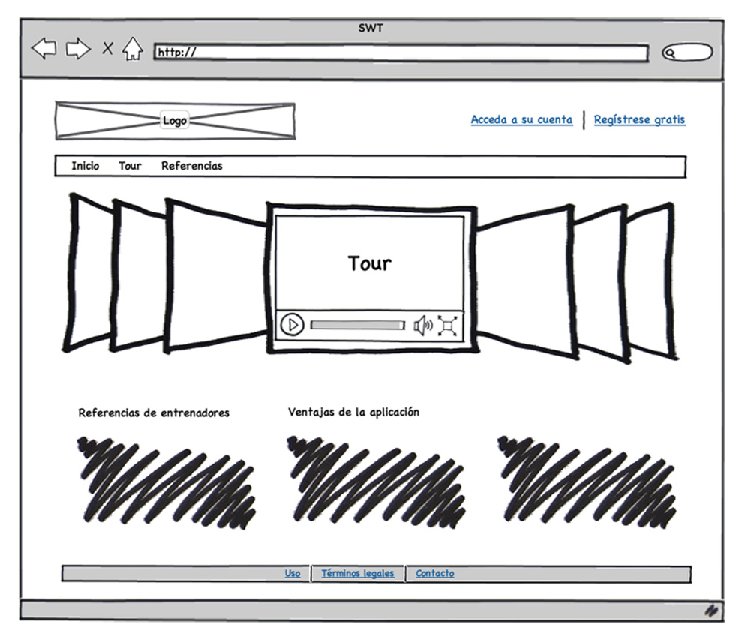
\includegraphics[width=8cm]{./eps/p_interfaz/1_Inicio.eps}
  	  \caption{Inicio en la interfaz pública}
  	  \label{fig:interfaz_publica_inicio}
  	\end{figure}

  	% subsection introducción (end)

  	\subsection{Interfaz pública} % (fold)
  		\label{sub:interfaz_publica}

  		La figura \ref{fig:interfaz_publica_inicio} muestra la estructura de la página web que actúa como interfaz pública. La parte superior está compuesta por el logo, enlace a registro/acceso a la aplicación y un menú para acceder al resto de páginas públicas a los entrenadores que aún no estén registrados en el sistema.

  		El resto de interfaces públicas que la conforman son: {\it tour} con las características y ventajas del sistema (figura \ref{fig:interfaz_publica_tour}); {\it referencias} de los entrenadores que participan en la elaboración del proyecto; página de {\it contacto} (figura \ref{fig:interfaz_publica_contacto}) con los administradores; {\it términos legales y de uso}. 

  		\begin{figure}[H]
  		  \centering
  		    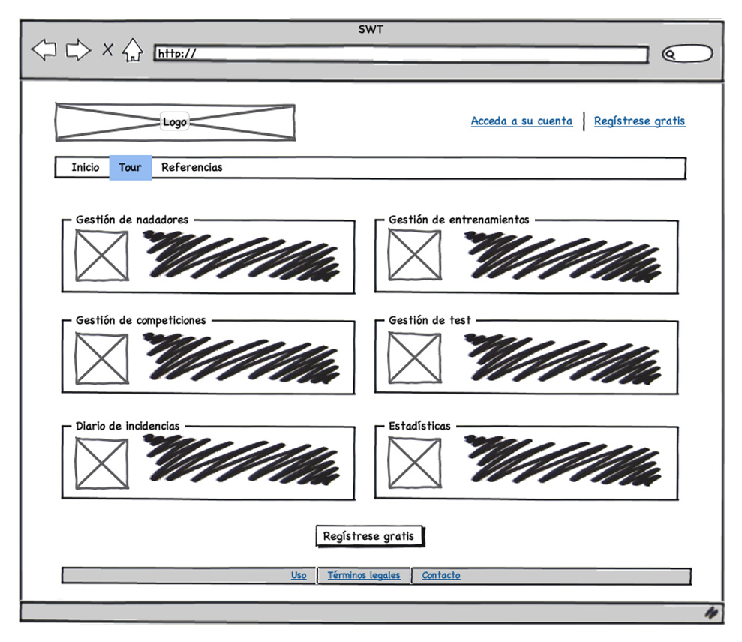
\includegraphics[width=8cm]{./eps/p_interfaz/2_Tour.eps}
  		  \caption{Tour en la interfaz pública}
  		  \label{fig:interfaz_publica_tour}
  		\end{figure}

  		\begin{figure}[H]
  		  \centering
  		    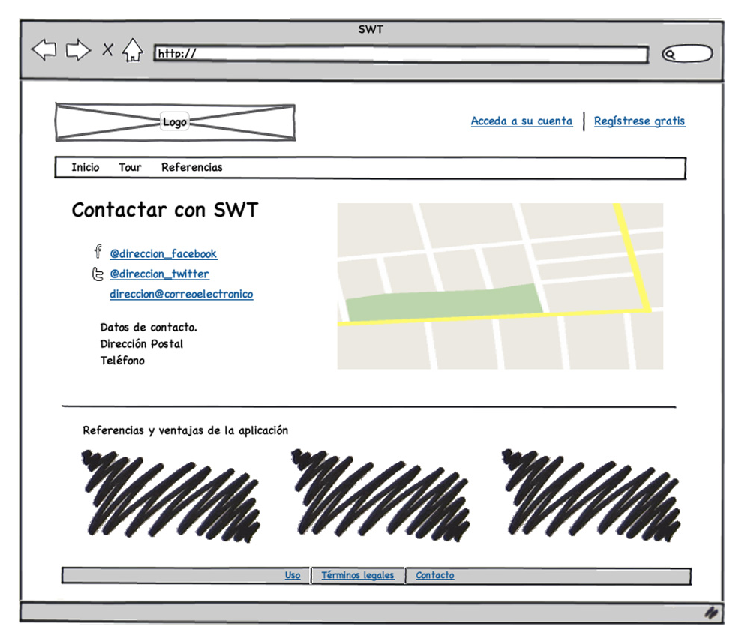
\includegraphics[width=8cm]{./eps/p_interfaz/3_Contacto.eps}
  		  \caption{Contacto en la interfaz pública}
  		  \label{fig:interfaz_publica_contacto}
  		\end{figure}

  	% subsection interfaz_pública (end)

  	\subsection{Registro y acceso} % (fold)
  		\label{sub:registro_y_acceso}

  		Las interfaces para el registro (figura \ref{fig:interfaz_registro}) y acceso (figura \ref{fig:interfaz_acceso}) de un entrenador al sistema son muy similares. Su estructura es algo diferente al resto de páginas de la aplicación, eliminando elementos que puedan interferir en el objetivo último ---registrarse o acceder. Hay que destacar que para el acceso, el identificador de usuario viene proporcionado por el correo electrónico insertado en la fase de registro.

  		\begin{figure}[H]
  		  \centering
  		    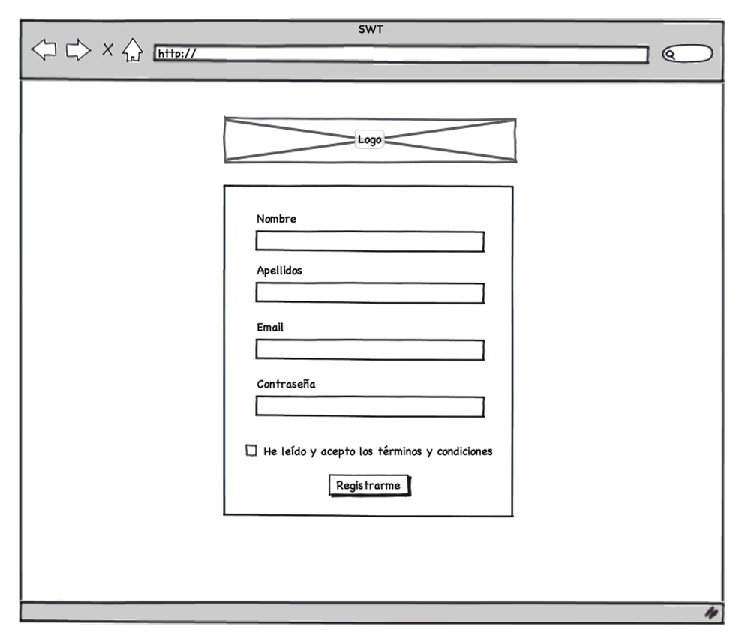
\includegraphics[width=8cm]{./eps/p_interfaz/4_Registro.eps}
  		  \caption{Interfaz para el registro de un entrenador}
  		  \label{fig:interfaz_registro}
  		\end{figure}

  		\begin{figure}[H]
  		  \centering
  		    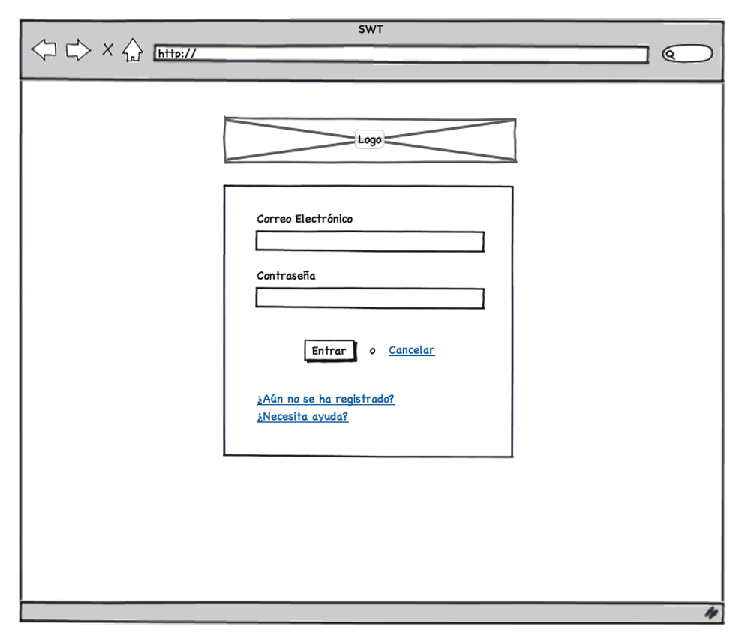
\includegraphics[width=8cm]{./eps/p_interfaz/5_Acceder.eps}
  		  \caption{Interfaz para el acceso de un entrenador}
  		  \label{fig:interfaz_acceso}
  		\end{figure}
  	% subsection registro_y_acceso (end)

  	\subsection{Dashboard} % (fold)
  		\label{sub:interfaz_dashboard}

  	Cuando el entrenador se registra en la aplicación, la primera página a la que accede es la de {\it dashboard} o resumen (figura \ref{fig:interfaz_dashboard}). En ella, lo primero que aparece es un recordatorio de los pasos que tiene que hacer para empezar a sacar provecho de la aplicación. A diferencia de las páginas vistas hasta el momento, ésta incluye en su estructura una barra lateral con los accesos que más frecuentemente se usan.

  		\begin{figure}[H]
  		  \centering
  		    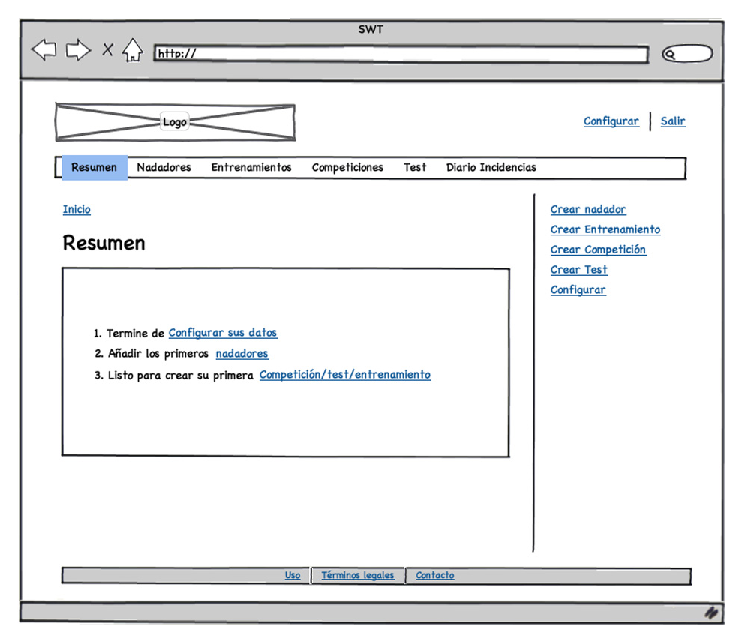
\includegraphics[width=8cm]{./eps/p_interfaz/6_Dashboard.eps}
  		  \caption{Interfaz para el dashboard de un entrenador}
  		  \label{fig:interfaz_dashboard}
  		\end{figure}

  	% subsection dashboard (end)

  	\subsection{Configuración del perfil} % (fold)
  		\label{sub:configuracion_del_perfil}

  	Cada entrenador registrado tiene un perfil asociado, donde se guarda información del tipo personal (figura \ref{fig:interfaz_conf_personal}), de contacto (figura \ref{fig:interfaz_conf_contacto}) y los parámetros relacionados con el índice de Mujika (figura \ref{fig:interfaz_conf_mujika}). La información está estructurada en pestañas para una mayor facilidad de navegación.

  		\begin{figure}[H]
  		  \centering
  		    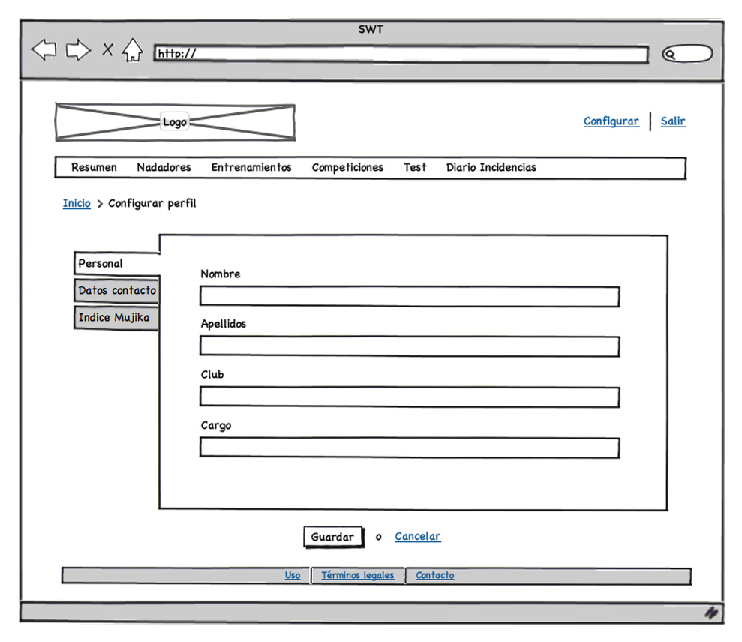
\includegraphics[width=8cm]{./eps/p_interfaz/7_Conf_personal.eps}
  		  \caption{Interfaz para la configuración de la información personal en el perfil}
  		  \label{fig:interfaz_conf_personal}
  		\end{figure}

  		\begin{figure}[H]
  		  \centering
  		    \includegraphics[width=8cm]{./eps/p_interfaz/8_Conf_contacto.eps}
  		  \caption{Interfaz para la configuración de la información de contacto en el perfil}
  		  \label{fig:interfaz_conf_contacto}
  		\end{figure}

  		\begin{figure}[H]
  		  \centering
  		    \includegraphics[width=8cm]{./eps/p_interfaz/9_Conf_mujika.eps}
  		  \caption{Interfaz para la configuración del índice de Mujika en el perfil}
  		  \label{fig:interfaz_conf_mujika}
  		\end{figure}

  	% subsection configuración_del_perfil (end)

  	\subsection{Gestión de nadadores} % (fold)
  		\label{sub:gestion_de_nadadores}

  	Uno de los módulos fundamentales en la aplicación es el de gestión de nadadores. Es, en gran medida, la base para las competiciones y los test, puesto que los resultados que se insertan en ellos dependen de los nadadores que un entrenador maneja. 

  	La estructura de la interfaz es común al resto de módulos y está compuesta de:

  	\begin{itemize}
  		\item {{\bf Tabla}. Muestra los registros insertados por un entrenador pertenecientes al módulo en que se encuentre. En este caso, como se está en la sección de nadadores, aparece el conjunto de nadadores que el entrenador ha dado de alta en el sistema.}
  		\item {{\bf Buscador}. Campo de búsqueda que localiza registros por diferentes parámetros.}
  		\item {{\bf Resumen}. Muestra información relevante al módulo en que se encuentre. Lo normal es que aparezca el número de registros insertados en cada módulo.}
  		\item {{\bf Barra lateral}. Desde ella se accede a cada una de las opciones del módulo que se esté gestionando.}
  	\end{itemize}

  	A continuación se muestran las interfaces de {\it ver listado de nadadores} (figura \ref{fig:interfaz_nadadores}), {\it añadir nadador} (figura \ref{fig:interfaz_nadadores_new}), {\it ver nadador} (figura \ref{fig:interfaz_nadadores_show}) y {\it modificar nadador} (figura \ref{fig:interfaz_nadadores_modif}). La primera de ellas muestra todos los nadadores insertados en la aplicación por un entrenador registrado; la segunda refleja el proceso para añadir un nuevo nadador; y la tercera como se modificaría. Es destacable que la información relacionada con las competiciones y test que aparece en {\it ver nadador}, no pueden ser modificadas desde este módulo, sino desde los que gestionan las competiciones y test.

  	\begin{figure}[H]
  	  \centering
  	    \includegraphics[width=8cm]{./eps/p_interfaz/10_Nadadores.eps}
  	  \caption{Interfaz para ver listado de nadadores}
  	  \label{fig:interfaz_nadadores}
  	\end{figure}

  	\begin{figure}[H]
  	  \centering
  	    \includegraphics[width=8cm]{./eps/p_interfaz/11_Nadadores_new.eps}
  	  \caption{Interfaz para añadir nadador}
  	  \label{fig:interfaz_nadadores_new}
  	\end{figure}

  	\begin{figure}[H]
  	  \centering
  	    \includegraphics[width=8cm]{./eps/p_interfaz/12_Nadadores_show.eps}
  	  \caption{Interfaz para ver nadador}
  	  \label{fig:interfaz_nadadores_show}
  	\end{figure}

  	\begin{figure}[H]
  	  \centering
  	    \includegraphics[width=8cm]{./eps/p_interfaz/13_Nadadores_modif.eps}
  	  \caption{Interfaz para modificar nadador}
  	  \label{fig:interfaz_nadadores_modif}
  	\end{figure}
  	% subsection gestión_de_nadadores (end)

  	\subsection{Gestión de Competiciones} % (fold)
  		\label{sub:gestion_de_competiciones}

  	La figura \ref{fig:interfaz_competiciones} muestra la interfaz para ver las competiciones añadidas por un entrenador registrado. Su estructura, como se especificó anteriormente, es similar a la del resto de módulos. La particularidad que tiene es que aparece un calendario de la temporada. A medida que se {\it añadan competiciones} (figura \ref{fig:interfaz_competiciones_new}) irán apareciendo ahí. 

  		\begin{figure}[H]
  		  \centering
  		    \includegraphics[width=8cm]{./eps/p_interfaz/14_Competiciones.eps}
  		  \caption{Interfaz para ver listado de competiciones}
  		  \label{fig:interfaz_competiciones}
  		\end{figure}

  		\begin{figure}[H]
  		  \centering
  		    \includegraphics[width=8cm]{./eps/p_interfaz/15_Competiciones_new.eps}
  		  \caption{Interfaz para añadir competición}
  		  \label{fig:interfaz_competiciones_new}
  		\end{figure}

  Cuando un entrenador hace clic sobre el nombre de la competición en la tabla, se accede a {\it ver una competición} (figura \ref{fig:interfaz_competiciones_show}). Cuando se modifica una competición (figura \ref{fig:interfaz_competiciones_modif}), se da la posibilidad de modificar cada uno de los resultados añadidos a la misma. Esta información es la que aparecerá modificada en la ficha de cada nadador.

  		\begin{figure}[H]
  		  \centering
  		    \includegraphics[width=8cm]{./eps/p_interfaz/16_Competiciones_show.eps}
  		  \caption{Interfaz para ver competición}
  		  \label{fig:interfaz_competiciones_show}
  		\end{figure}

  		\begin{figure}[H]
  		  \centering
  		    \includegraphics[width=8cm]{./eps/p_interfaz/17_Competiciones_modif.eps}
  		  \caption{Interfaz para modificar competición}
  		  \label{fig:interfaz_competiciones_modif}
  		\end{figure}
  	% subsection gestión_de_competiciones (end)

  	\subsection{Gestión de entrenamientos} % (fold)
  		\label{sub:gestion_de_entrenamientos}

  		\begin{figure}[H]
  		  \centering
  		    \includegraphics[width=8cm]{./eps/p_interfaz/18_Entrenamientos.eps}
  		  \caption{Interfaz para ver listado de entrenamientos}
  		  \label{fig:interfaz_entrenamientos}
  		\end{figure}

  	La {\it lista de entrenamientos} (figura \ref{fig:interfaz_entrenamientos}) refleja cada una de las sesiones que inserta el entrenador a lo largo de una temporada. En el resumen se muestran la cantidad de sesiones, el volumen y la carga realizadas en total. Al hacer clic sobre el nombre del entrenamiento, se accede a {\it ver entrenamiento} (figura \ref{fig:interfaz_entrenamientos_show}), que incluye cada uno de los ejercicios añadidos al mismo. Como cada ejercicio tiene asociado un volumen y una carga, se muestra el total de esa sesión. Esto ayuda al entrenador a la hora de hacer los entrenamientos, puesto que conoce el estado a medida que los va desarrollando.\\
  	\newline
  	{\it Añadir} (figura \ref{fig:interfaz_entrenamientos_new}) y {\it modificar entrenamiento} son iguales, con la salvedad de que el segundo permite cambiar los datos de los formularios que se agregan en el primero.

  		\begin{figure}[H]
  		  \centering
  		    \includegraphics[width=8cm]{./eps/p_interfaz/20_Entrenamientos_show.eps}
  		  \caption{Interfaz para ver entrenamiento}
  		  \label{fig:interfaz_competiciones_show}
  		\end{figure}

  		\begin{figure}[H]
  		  \centering
  		    \includegraphics[width=8cm]{./eps/p_interfaz/19_Entrenamientos_new.eps}
  		  \caption{Interfaz para añadir entrenamiento}
  		  \label{fig:interfaz_entrenamientos_new}
  		\end{figure}

  	% subsection gestión_de_entrenamientos (end)

  	\subsection{Gestión de test} % (fold)
  		\label{sub:gestion_de_test}

  	Al igual que para las competiciones, la gestión de test (figura \ref{fig:interfaz_test}) se realiza de la misma forma. La diferencia fundamental está en la información que aparece en la tabla de test insertados por el entrenador en la aplicación. Como para las competiciones, cada uno de los resultados asociados a cada test, aparecen en la ficha de cada nadador.

  		\begin{figure}[H]
  		  \centering
  		    \includegraphics[width=8cm]{./eps/p_interfaz/26_Test.eps}
  		  \caption{Interfaz para ver listado de test}
  		  \label{fig:interfaz_test}
  		\end{figure}
  	% subsection gestión_de_test (end)

  	\subsection{Gestión diario de incidencias} % (fold)
  		\label{sub:interfaz_gestion_diario_de_incidencias}

  	La interfaz para el diario de incidencias del entrenador difiere del resto en que, cada incidencia, tiene asociada una o varias etiquetas. Por ello, en el resumen que aparece en la interfaz de {\it ver diario de incidencias} (figura \ref{fig:interfaz_incidencias}), se muestran los valores más usados por los entrenadores. Esto ayudará a localizar rápidamente cada tipo de incidencia. Como en casos anteriores, a continuación se muestra {\it ver incidencia} (figura \ref{fig:interfaz_incidencias_show}), {\it añadir incidencia} (figura \ref{fig:interfaz_incidencias_new}) y {\it modificar incidencia} (figura \ref{fig:interfaz_incidencias_modif}).

  		\begin{figure}[H]
  		  \centering
  		    \includegraphics[width=8cm]{./eps/p_interfaz/22_Diario.eps}
  		  \caption{Interfaz para ver diario de incidencias}
  		  \label{fig:interfaz_incidencias}
  		\end{figure}

  		\begin{figure}[H]
  		  \centering
  		    \includegraphics[width=8cm]{./eps/p_interfaz/23_Diario_new.eps}
  		  \caption{Interfaz para añadir incidencia}
  		  \label{fig:interfaz_incidencias_new}
  		\end{figure}

  		\begin{figure}[H]
  		  \centering
  		    \includegraphics[width=8cm]{./eps/p_interfaz/24_Diario_show.eps}
  		  \caption{Interfaz para ver incidencia}
  		  \label{fig:interfaz_incidencias_show}
  		\end{figure}

  		\begin{figure}[H]
  		  \centering
  		    \includegraphics[width=8cm]{./eps/p_interfaz/25_Diario_modif.eps}
  		  \caption{Interfaz para modificar incidencia}
  		  \label{fig:interfaz_incidencias_modif}
  		\end{figure}
  	% subsection interfaz_gestión_diario_de_incidencias (end)
  % section diseño_de_interfaz_de_usuario (end)
  
	% ----------------------------------
	% Sec Diagramas clases
	% ----------------------------------
	\section{Diagramas de clases} % (fold)
		\label{sec:diagramas_de_clases}
		
		Una clase de diseño y sus objetos, y de ese modo también los subsistemas que contienen las clases de diseño, a menudo participan en varias realizaciones de casos de uso. También puede darse el caso de algunas operaciones, atributos y asociaciones sobre una clase específica que son relevantes para sólo una realización de caso de uso. Esto es importante para coordinar todos los requisitos que diferentes realizaciones de casos de uso imponen a una clase, a sus objetos y a los subsistemas que que contiene. Para manejar todo esto, se utilizan los diagramas de clases conectados a una realización de caso de uso, mostrando sus clases participantes, subsistemas y sus relaciones. 
		
		% ----------------------------------
		% Sub Patrón MVC
		% ----------------------------------
		\subsection{Patrón MVC} % (fold)
			\label{sub:patron_mvc}
			
			MVC es un patrón de diseño que considera dividir una aplicación en tres módulos claramente identificables y con funcionalidad bien definida: {\it el modelo, las vistas y el controlador}.
			
			\begin{itemize}
				\item {\bf El modelo} es un conjunto de clases que representan la información del mundo real que el sistema debe procesar, sin tomar en cuenta ni la forma en la que esa información va a ser mostrada ni los mecanismos que hacen que esos datos estén dentro del modelo, es decir, sin tener relación con ninguna otra entidad dentro de la aplicación. 
				\item {\bf Las vistas} son el conjunto de clases que se encargan de mostrar al usuario la información contenida en el modelo. Una vista está asociada a un modelo, pudiendo existir varias vistas asociadas al mismo modelo. Una vista obtiene del modelo solamente la información que necesita para desplegar y se actualiza cada vez que el modelo del dominio cambia por medio de notificaciones generadas por el modelo de la aplicación.
				\item {\bf El controlador} es un objeto que se encarga de dirigir el flujo del control de la aplicación debido a mensajes externos, como datos introducidos por el usuario u opciones del menú seleccionadas por él. A partir de estos mensajes, el controlador se encarga de modificar el modelo o de abrir y cerrar vistas. El controlador tiene acceso al modelo y a las vistas, pero las vistas y el modelo no conocen de la existencia del controlador.
			\end{itemize}			
			
			\begin{figure}[H]
			  \centering
			    \includegraphics[width=12cm]{./eps/di_diagclases/mvc.eps}
			  \caption{Disposición en el patrón MVC}
			  \label{fig:patron_MVC}
			\end{figure}
			
			Aunque se pueden encontrar diferentes implementaciones de MVC, el flujo que sigue el control generalmente es el siguiente:
			
			\begin{itemize}
				\item El usuario interactúa con la interfaz de usuario de alguna forma.
				\item El controlador recibe (por parte de los objetos de la interfaz-vista) la notificación de la acción solicitada por el usuario. El controlador gestiona el evento que llega. 
				\item El controlador accede al modelo, actualizándolo, posiblemente modificándolo de forma adecuada a la acción solicitada por el usuario. Los controladores complejos están a menudo estructurados usando un patrón de comando que encapsula las acciones y simplifica su extensión.
				\item El controlador delega a los objetos de la vista la tarea de desplegar la interfaz de usuario. La vista obtiene sus datos del modelo para generar la interfaz apropiada para el usuario donde se reflejan los cambios en el modelo. El modelo no debe tener conocimiento directo sobre la vista. El controlador no pasa objetos de dominio (el modelo) a la vista aunque puede dar la orden a la vista para que se actualice. 
				\item La interfaz de usuario espera nuevas interacciones del usuario, comenzando el ciclo nuevamente. 
			\end{itemize}
			
			La disposición de los paquetes de la aplicación se organizarán según el patrón MVC ({\it véase} Figura \ref{fig:patron_MVC}). Por ello, los modelos, los controladores y las vistas se encontrarán aisladas entre sí.
			
			Para simplificar el diagrama de clases de la aplicación, en la figura \ref{fig:di_diag_clases} se muestran las clases con los estereotipos usados en el {\it framework} de desarrollo, agrupando únicamente las pertenecientes al modelo.
			
			\begin{figure}[H]
			  \centering
			    \includegraphics[width=16cm]{./eps/di_diagclases/di_diagclases.eps}
			  \caption{Diagrama de clases para el diseño}
			  \label{fig:di_diag_clases}
			\end{figure}
			
			Los controladores se relacionan directamente con las vistas y los modelos, habiendo tal y como se explicó anteriormente, una separación lógica entre vistas y modelos.
			
			El {\bf Modelo} es donde residen los datos y es el encargado de acceder a los mismos. Se comunica con el gestor de bases de datos para que se realice todo el almacenamiento de estos. En las aplicaciones basadas en {\it Ruby on Rails}, la definición del modelo es sumamente importante, puesto que el modelo de negocio se sustenta en él.

    	 \begin{figure}[H]
    		  \centering
    		    \includegraphics[width=13cm]{./eps/di_modelo_er/ModeloER.eps}
    		  \caption{Estructuración del modelo de bases de datos}
    		  \label{fig:di_diag_despliegue}
    		\end{figure}
			
		% subsection patrón_mvc (end)
		
	% section diagramas_de_clases (end)
	
	% ----------------------------------
	% Sec Diagramas de Secuencia
	% ----------------------------------
	\section{Diagramas de secuencia} % (fold)
		\label{sec:diagramas_de_secuencia}
	
		Cómo fue explicado en capítulos anteriores, los diagramas de interacción son diagramas que describen cómo grupos de objetos colaboran para conseguir algún fin. Estos diagramas muestran objetos, así como los mensajes que se pasan entre ellos dentro del caso de uso, es decir, capturan el comportamiento de los casos de uso.
		
		La secuencia de acciones en un caso de uso comienza cuando un actor invoca el caso de uso mediante el envío de algún tipo de mensaje al sistema. Si se considera el <<interior>> del sistema, se tiene algún objeto de diseño que recibe el mensaje del actor. Después el objeto de diseño llama a algún otro objeto, y de esa manera los objetos implicados interactúan para realizar y llevar a cabo un caso de uso. En el diseño, es preferible representar esto con diagramas de secuencia, ya que el centro de atención principal es el encontrar secuencias de interacciones detalladas y ordenadas en el tiempo.
		
		Hay dos tipos de diagrama de interacción, ambos basados en la misma información, pero cada uno enfatizando un aspecto particular: {\bf Diagramas de Secuencia} y Diagramas de Colaboración.
		
		Un diagrama de secuencia muestra una interacción ordenada según la secuencia temporal de eventos. En particular, muestra los objetos participantes en la interacción y los mensajes que intercambian ordenados según su secuencia en el tiempo. Es decir, muestra la interacción de un conjunto de objetos en una aplicación a través del tiempo y se modela para cada caso de uso.
		
		A continuación se detallarán dos diagramas de secuencia que hacen referencia a la cada uno de los módulos detallados en la fase de análisis (capítulo \ref{cha:analisis}).
		
		Se recuerda al lector que los paquetes principales son:
		\begin{itemize}
		  \item Gestión de nadadores
		  \item Gestión de competiciones
		  \item Gestión de test
		  \item Gestión del diario de incidencias
		\end{itemize}
		
		% ----------------------------------
		% Sub Diagrama secuencia añadir nadador
		% ----------------------------------
		\subsection{Diagrama secuencia añadir nadador} % (fold)
		\label{sub:diagrama_secuencia_anadir_nadador}
			
			En el diagrama de secuencia de la figura \ref{fig:di_sec_anadirnadador} se muestra el flujo de acciones correspondiente para poder crear un nuevo nadador en el sistema.
			
			La clase {\it Vista Nadador} engloba las vistas correspondientes a cada uno de los métodos del controlador de nadadores. Así, por ejemplo, al método {\it index} del controlador le corresponde una vista {\it index.html.erb}. Es fundamental conocer esto para entender que en las acciones 3 y 7 el controlador envía la acción de renderizar las vistas correspondientes a los métodos {\it new y show}, debido a que son los que se ejecutan dentro de la clase.
			
			La clase {\it nadador} correspondiente al modelo es la encargada de detectar si es posible la creación de un nuevo registro o no en la base de datos. En caso de no ser posible, notifica al controlador y éste muestra un mensaje de error en la vista. En caso de que todo vaya bien, se muestra el nuevo registro creado con la ficha del nadador.
			
			\begin{figure}[H]
			  \centering
			    \includegraphics[width=15cm]{./eps/di_diagsecuencia/Nadador_Anadir.eps}
			  \caption{Diagrama de secuencia para añadir un nadador}
			  \label{fig:di_sec_anadirnadador}
			\end{figure}
			
		% subsection diagrama_secuencia_añadir_nadador (end) 
		
		% ----------------------------------
		% Sub Diagrama secuencia ver nadador
		% ----------------------------------
		\subsection{Diagrama secuencia ver nadador} % (fold)
		\label{sub:diagrama_secuencia_ver_nadador}
		
			En el diagrama de secuencia de la figura \ref{fig:di_sec_anadirnadador} se muestra el flujo de acciones correspondiente para poder ver un nadador perteneciente a un entrenador registrado.
			
			La secuencia comienza cuando el entrenador registrado solicita ver el listado de nadadores que ha añadido al sistema. Es requisito el ver el listado para poder posteriormente seleccionar un nadador concreto. Para ver todo el conjunto de nadadores, el controlador obtiene del modelo todos los nadadores y los muestra al renderizar {\it index.html.erb}. 
			
			El siguiente paso es el {\it seleccionar un nadador} concreto. Se hace una llamada al método {\it show}, el cuál pedirá al modelo el nadador concreto seleccionado. El modelo devuelve los datos del nadador y el controlador renderizará la ficha del mismo.
			
			Requisitos que se tendrán que contemplar en la fase de implementación:
			
			\begin{itemize}
			 \item No se puede acceder a un nadador perteneciente a otro nadador.
			 \item En caso de no poderse acceder, se mostrará mensaje de error.
			\end{itemize}
			
			\begin{figure}[H]
			  \centering
			    \includegraphics[width=15cm]{./eps/di_diagsecuencia/Nadador_Ver.eps}
			  \caption{Diagrama de secuencia para ver un nadador}
			  \label{fig:di_sec_vernadador}
			\end{figure}
		
		% subsection diagrama_secuencia_ver_lista_de_nadadores (end)
		
		% ----------------------------------
		% Sub Diagrama secuencia eliminar nadador
		% ----------------------------------
		\subsection{Diagrama secuencia eliminar nadador} % (fold)
		  \label{sub:diagrama_secuencia_eliminar_nadador}
		
		  En el diagrama de secuencia de la figura \ref{fig:di_sec_eliminarnadador} se muestra el flujo de acciones correspondiente para poder eliminar un nadador del sistema.
		  
		  Primeramente el entrenador ve la lista de nadadores insertados en el sistema a través de la clase {\it Vista Nadador}. Esto es requisito para poder seleccionar el candidato a eliminar. Una vez elegido, se lanzará el método {\it destroy} desde el controlador, el cuál indicará al modelo que se destruya el registro almacenado en el modelo. Así mismo, se realizará el correspondiente borrado en cascada de la información correspondiente a los resultados almacenados sobre competiciones y test pertenecientes al nadador.
		  
		  \begin{figure}[H]
			  \centering
			    \includegraphics[width=15cm]{./eps/di_diagsecuencia/Nadador_Eliminar.eps}
			  \caption{Diagrama de secuencia para eliminar un nadador}
			  \label{fig:di_sec_eliminarnadador}
			\end{figure}
		% subsection diagrama_secuencia_eliminar_nadador (end)
		
		% ----------------------------------
		% Sub Diagrama secuencia modificar nadador
		% ----------------------------------
		\subsection{Diagrama secuencia modificar nadador} % (fold)
		  \label{sub:diagrama_secuencia_modificar_nadador}
		  
		  En el diagrama de secuencia de la figura \ref{fig:di_sec_modificarnadador} se muestra el flujo de acciones correspondiente para poder modificar un nadador perteneciente a un entrenador determinado del sistema.
		  
		  El flujo de sucesos comienza con la selección por parte del entrenador de la opción {\it Ver lista de nadadores}. Una vez mostrados, se selecciona el candidato a modificar. Es el propio controlador quien llama primeramente al método {\it edit}, donde se muestra un formulario con los datos del nadador almacenados en el modelo. Posteriormente, el {\it Controlador Nadador} renderizará la vista para poder editar los datos.
		
		  Requisito que se tendrá que contemplar en la fase de implementación:
			
			\begin{itemize}
			 \item Únicamente se podrán modificar los datos del modelo de nadador en la {\it Vista Entrenamiento}. Los resultados en competiciones y test no se podrán cambiar desde esta vista.
			\end{itemize}
			
		  \begin{figure}[H]
			  \centering
			    \includegraphics[width=15cm]{./eps/di_diagsecuencia/Nadador_Modificar.eps}
			  \caption{Diagrama de secuencia para modificar un nadador}
			  \label{fig:di_sec_modificarnadador}
			\end{figure}
			
			\newpage
		% subsection diagrama_secuencia_modificar_nadador (end)
		
		% ----------------------------------
		% Sub Diagrama secuencia añadir entrenamiento
		% ----------------------------------
		\subsection{Diagrama secuencia añadir entrenamiento} % (fold)
		  \label{sub:diagrama_secuencia_anadir_entrenamiento}
		  
		  En el diagrama de secuencia de la figura \ref{fig:di_sec_anadirentrenamiento} se muestra el flujo de acciones correspondiente para poder añadir un entrenamiento perteneciente a un entrenador al sistema.
		  
		  El entrenador registrado selecciona la opción de {\it Añadir Entrenamiento} de la {\it Vista Entrenamiento}. Automáticamente, la aplicación enrutará \footnote{El framework rails utiliza un enrutador para guiar el proceso RESTful con cada una de las cabeceras HTTP} el método {\it new} para cargar las vistas con el formulario de un nuevo entrenamiento.
		  
		  El entrenador rellenará el formulario y lo enviará a través del método {\it create}. Será éste el encargado de crear un nuevo entrenamiento en el modelo de {\it Entrenamiento} y, si previamente se han creado ejercicios asociados al mismo, en el de {\it Ejercicios}.
		  
		  \begin{figure}[H]
			  \centering
			    \includegraphics[width=15cm]{./eps/di_diagsecuencia/Entrenamiento_Anadir.eps}
			  \caption{Diagrama de secuencia para añadir un entrenamiento}
			  \label{fig:di_sec_anadirentrenamiento}
			\end{figure}
		
		  \newpage
		% subsection diagrama_secuencia_añadir_entrenamiento (end)
		
		% ----------------------------------
		% Sub Diagrama secuencia ver entrenamiento
		% ----------------------------------
		\subsection{Diagrama secuencia ver entrenamiento} % (fold)
		  \label{sub:diagrama_secuencia_ver_entrenamiento}
		  
		  En el diagrama de secuencia de la figura \ref{fig:di_sec_verentrenamiento} se muestra el flujo de acciones correspondiente para poder ver un entrenamiento perteneciente a un entrenador al sistema.
		  
		  Al igual que en procesos anteriores, para poder ver un entrenamiento previamente se ha seleccionado de una lista. Tras la selección, el controlador busca en el modelo por identificador tanto el entrenamiento como los ejercicios asociados al mismo.
		  
		  Requisitos que se tendrán que contemplar en la fase de implementación:
			
			\begin{itemize}
			 \item No se puede acceder a un entrenamiento perteneciente a otro nadador.
			 \item En caso de no poderse acceder, se mostrará mensaje de error.
			\end{itemize}
			
		  \begin{figure}[H]
			  \centering
			    \includegraphics[width=15cm]{./eps/di_diagsecuencia/Entrenamiento_Ver.eps}
			  \caption{Diagrama de secuencia para ver un entrenamiento}
			  \label{fig:di_sec_verentrenamiento}
			\end{figure}
		
		\newpage
		% subsection diagrama_secuencia_ver_entrenamiento (end)
		
		% ----------------------------------
		% Sub Diagrama secuencia para eliminar entrenamiento
		% ----------------------------------
		\subsection{Diagrama secuencia eliminar entrenamiento} % (fold)
		  \label{sub:diagrama_secuencia_eliminar_entrenamiento}
		
		  En el diagrama de secuencia de la figura \ref{fig:di_sec_eliminarentrenamiento} se muestra el flujo de acciones correspondiente para poder eliminar un entrenamiento perteneciente a un entrenador al sistema.
		  
		  Tras seleccionar el entrenamiento a eliminar del listado de entrenamientos totales, la vista hace una llamada al método {\it destroy} del controlador. Éste elimina el registro seleccionado del modelo y posteriormente, los ejercicios asociados al mismo.
		  
		  Aunque para el caso de nadadores (sección \ref{sub:diagrama_secuencia_eliminar_nadador}) no se explicó, surgió la misma analogía que aparecerá en este diagrama. A la hora de borrar los ejercicios, Rails usando el patrón {\it Active Record} (ver sección \ref{ssub:ror_active_record}) genera parte de lo que se conoce como «magia». Internamente el framework implementa un procedimiento para acceder a los ejercicios asociados a un entrenamiento y, a su vez, de habilitar un procedimiento para borrarlos todos.
		  
		  \begin{figure}[H]
			  \centering
			    \includegraphics[width=15cm]{./eps/di_diagsecuencia/Entrenamiento_Eliminar.eps}
			  \caption{Diagrama de secuencia para eliminar un entrenamiento}
			  \label{fig:di_sec_eliminarentrenamiento}
			\end{figure}
		
		  \newpage
		% subsection diagrama_secuencia_para_eliminar_entrenamiento (end)
		
		% ----------------------------------
		% Sub Diagrama secuencia para modificar entrenamiento
		% ----------------------------------
		\subsection{Diagrama secuencia modificar entrenamiento} % (fold)
		  \label{sub:diagrama_secuencia_modificar_entrenamiento}
		  
		  En el diagrama de secuencia de la figura \ref{fig:di_sec_modificarentrenamiento} se muestra el flujo de acciones correspondiente para poder modificar un entrenamiento perteneciente a un entrenador al sistema.
		  
		  \begin{figure}[H]
			  \centering
			    \includegraphics[width=15cm]{./eps/di_diagsecuencia/Entrenamiento_Modificar.eps}
			  \caption{Diagrama de secuencia para modificar un entrenamiento}
			  \label{fig:di_sec_modificarentrenamiento}
			\end{figure}
			
			\newpage
		% subsection diagrama_secuencia_para_modificar_entrenamiento (end)
		
		% ----------------------------------
		% Sub Diagrama secuencia para añadir competición
		% ----------------------------------
		\subsection{Diagrama secuencia añadir competición} % (fold)
		  \label{sub:diagrama_secuencia_anadir_competicion}
		
		  En el diagrama de secuencia de la figura \ref{fig:di_sec_anadircompeticion} se muestra el flujo de acciones correspondiente para poder añadir una competición perteneciente a un entrenador al sistema.
		  
		  \begin{figure}[H]
			  \centering
			    \includegraphics[width=15cm]{./eps/di_diagsecuencia/Competicion_Anadir.eps}
			  \caption{Diagrama de secuencia para añadir una competición}
			  \label{fig:di_sec_anadircompeticion}
			\end{figure}
			
			\newpage
		% subsection diagrama_secuencia_para_añadir_competición (end)
		
		% ----------------------------------
		% Sub Diagrama secuencia para ver competición
		% ----------------------------------
		\subsection{Diagrama secuencia ver competición} % (fold)
		  \label{sub:diagrama_secuencia_ver_competicion}
		  
		  En el diagrama de secuencia de la figura \ref{fig:di_sec_vercompeticion} se muestra el flujo de acciones correspondiente para poder ver una competición perteneciente a un entrenador al sistema.
		  
		  \begin{figure}[H]
			  \centering
			    \includegraphics[width=15cm]{./eps/di_diagsecuencia/Competicion_Ver.eps}
			  \caption{Diagrama de secuencia para ver una competición}
			  \label{fig:di_sec_vercompeticion}
			\end{figure}
		
		  \newpage
		% subsection diagrama_secuencia_para_ver_competición (end)
		
		% ----------------------------------
		% Sub Diagrama secuencia para eliminar competición
		% ----------------------------------
		\subsection{Diagrama secuencia eliminar competición} % (fold)
		  \label{sub:diagrama_secuencia_eliminar_competicion}
		  
		  En el diagrama de secuencia de la figura \ref{fig:di_sec_eliminarcompeticion} se muestra el flujo de acciones correspondiente para poder eliminar una competición perteneciente a un entrenador al sistema.
		  
		  \begin{figure}[H]
			  \centering
			    \includegraphics[width=15cm]{./eps/di_diagsecuencia/Competicion_Eliminar.eps}
			  \caption{Diagrama de secuencia para eliminar una competición}
			  \label{fig:di_sec_eliminarcompeticion}
			\end{figure}
		
		  \newpage
		% subsection diagrama_secuencia_para_eliminar_competición (end)
		
		% ----------------------------------
		% Sub Diagrama secuencia para modificar competición
		% ----------------------------------
		\subsection{Diagrama secuencia modificar competición} % (fold)
		  \label{sub:diagrama_secuencia_modificar_competicion}
		  
		  En el diagrama de secuencia de la figura \ref{fig:di_sec_modificarcompeticion} se muestra el flujo de acciones correspondiente para poder modificar una competición perteneciente a un entrenador al sistema.
		  
		  \begin{figure}[H]
			  \centering
			    \includegraphics[width=15cm]{./eps/di_diagsecuencia/Competicion_Modificar.eps}
			  \caption{Diagrama de secuencia para modificar una competición}
			  \label{fig:di_sec_modificarcompeticion}
			\end{figure}
		
		  \newpage
		% subsection diagrama_secuencia_para_modificar_competición (end)
		
		% ----------------------------------
		% Sub Diagrama secuencia para añadir test
		% ----------------------------------
		\subsection{Diagrama secuencia añadir test} % (fold)
		  \label{sub:diagrama_secuencia_anadir_test}
		
		  En el diagrama de secuencia de la figura \ref{fig:di_sec_anadirtest} se muestra el flujo de acciones correspondiente para poder añadir un test perteneciente a un entrenador al sistema.
		  
		  \begin{figure}[H]
			  \centering
			    \includegraphics[width=15cm]{./eps/di_diagsecuencia/Test_Anadir.eps}
			  \caption{Diagrama de secuencia para añadir un test}
			  \label{fig:di_sec_anadirtest}
			\end{figure}
			
			\newpage
		% subsection diagrama_secuencia_para_añadir_test (end)
		
		% ----------------------------------
		% Sub Diagrama secuencia para ver test
		% ----------------------------------
		\subsection{Diagrama secuencia ver test} % (fold)
		  \label{sub:diagrama_secuencia_ver_test}
		  
		  En el diagrama de secuencia de la figura \ref{fig:di_sec_vertest} se muestra el flujo de acciones correspondiente para poder ver un test perteneciente a un entrenador al sistema.
		  
		  \begin{figure}[H]
			  \centering
			    \includegraphics[width=15cm]{./eps/di_diagsecuencia/Test_Ver.eps}
			  \caption{Diagrama de secuencia para ver un test}
			  \label{fig:di_sec_vertest}
			\end{figure}
		
		  \newpage
		% subsection diagrama_secuencia_para_ver_test (end)
		
		% ----------------------------------
		% Sub Diagrama secuencia para eliminar test
		% ----------------------------------
		\subsection{Diagrama secuencia eliminar test} % (fold)
		  \label{sub:diagrama_secuencia_eliminar_test}
		
		  En el diagrama de secuencia de la figura \ref{fig:di_sec_eliminartest} se muestra el flujo de acciones correspondiente para poder añadir un eliminar perteneciente a un entrenador al sistema.
		  
		  \begin{figure}[H]
			  \centering
			    \includegraphics[width=15cm]{./eps/di_diagsecuencia/Test_Eliminar.eps}
			  \caption{Diagrama de secuencia para eliminar un test}
			  \label{fig:di_sec_eliminartest}
			\end{figure}
			
			\newpage
		% subsection diagrama_secuencia_para_eliminar_test (end)
		
		% ----------------------------------
		% Sub Diagrama secuencia para modificar test
		% ----------------------------------
		\subsection{Diagrama secuencia modificar test} % (fold)
		  \label{sub:diagrama_secuencia_modificar_test}
		
		  En el diagrama de secuencia de la figura \ref{fig:di_sec_modificartest} se muestra el flujo de acciones correspondiente para poder modificar un test perteneciente a un entrenador al sistema.
		  
		  \begin{figure}[H]
			  \centering
			    \includegraphics[width=15cm]{./eps/di_diagsecuencia/Test_Modificar.eps}
			  \caption{Diagrama de secuencia para modificar un test}
			  \label{fig:di_sec_modificartest}
			\end{figure}
			
			\newpage
		% subsection diagrama_secuencia_para_modificar_test (end)
		
		% ----------------------------------
		% Sub Diagrama secuencia añadir incidencia
		% ----------------------------------
		\subsection{Diagrama secuencia añadir incidencia} % (fold)
		  \label{sub:diagrama_secuencia_anadir_incidencia}
		
		  En el diagrama de secuencia de la figura \ref{fig:di_sec_anadirincidencia} se muestra el flujo de acciones correspondiente para poder añadir una incidencia perteneciente a un entrenador al sistema.
		  
		  \begin{figure}[H]
			  \centering
			    \includegraphics[width=15cm]{./eps/di_diagsecuencia/RegistroInc_Anadir.eps}
			  \caption{Diagrama de secuencia para modificar una incidencia}
			  \label{fig:di_sec_anadirincidencia}
			\end{figure}
			
			\newpage
		% subsection diagrama_secuencia_añadir_incidencia (end)
		
		% ----------------------------------
		% Sub Diagrama secuencia ver incidencia
		% ----------------------------------
		\subsection{Diagrama secuencia ver incidencia} % (fold)
		  \label{sub:diagrama_secuencia_ver_incidencia}
		
		  En el diagrama de secuencia de la figura \ref{fig:di_sec_verincidencia} se muestra el flujo de acciones correspondiente para poder ver una incidencia perteneciente a un entrenador al sistema.
		  
		  \begin{figure}[H]
			  \centering
			    \includegraphics[width=15cm]{./eps/di_diagsecuencia/RegistroInc_Ver.eps}
			  \caption{Diagrama de secuencia para ver una incidencia}
			  \label{fig:di_sec_verincidencia}
			\end{figure}
			
			\newpage
		% subsection diagrama_secuencia_ver_incidencia (end)
		
		% ----------------------------------
		% Sub Diagrama secuencia eliminar incidencia
		% ----------------------------------
		\subsection{Diagrama secuencia eliminar incidencia} % (fold)
		  \label{sub:diagrama_secuencia_eliminar_incidencia}
		
		  En el diagrama de secuencia de la figura \ref{fig:di_sec_eliminarincidencia} se muestra el flujo de acciones correspondiente para poder eliminar una incidencia perteneciente a un entrenador al sistema.
		  
		  \begin{figure}[H]
			  \centering
			    \includegraphics[width=15cm]{./eps/di_diagsecuencia/RegistroInc_Eliminar.eps}
			  \caption{Diagrama de secuencia para eliminar una incidencia}
			  \label{fig:di_sec_eliminarincidencia}
			\end{figure}
			
			\newpage
		% subsection diagrama_secuencia_eliminar_incidencia (end)
		
		% ----------------------------------
		% Sub Diagrama secuencia modificar incidencia
		% ----------------------------------
		\subsection{Diagrama secuencia modificar incidencia} % (fold)
		  \label{sub:diagrama_secuencia_modificar_incidencia}
		
		  En el diagrama de secuencia de la figura \ref{fig:di_sec_modificarincidencia} se muestra el flujo de acciones correspondiente para poder modificar una incidencia perteneciente a un entrenador al sistema.
		  
		  \begin{figure}[H]
			  \centering
			    \includegraphics[width=15cm]{./eps/di_diagsecuencia/RegistroInc_Modificar.eps}
			  \caption{Diagrama de secuencia para modificar una incidencia}
			  \label{fig:di_sec_modificarincidencia}
			\end{figure}
			
		% subsection diagrama_secuencia_modificar_incidencia (end)
	% section diagramas_de_secuencia (end)

	% ----------------------------------
	% Sec Diagrama de paquetes
	% ----------------------------------
	\section{Diagrama de paquetes} % (fold)
		\label{sec:diagrama_de_paquetes_diseno}
	
		En la sección \ref{sec:diagrama_de_paquetes_analisis} de la fase de análisis se hace una primera aproximación de las capas necesarias de la aplicación. Se hizo referencia a una arquitectura en 4 capas donde se detalló la composición de las capas genérica y específica. El siguiente paso es identificar los subsistemas intermedios y de software del sistema.
		
		El software del sistema y la capa intermedia constituyen los cimientos de un sistema, ya que toda la funcionalidad descansa sobre software como sistemas operativos, sistemas de gestión de bases de datos, software de comunicaciones, tecnologías de distribución de objetos, kits de diseño de IGU y tecnologías de gestión de transacciones. La selección e integración de productos software que se comprar o se construyen son dos de los objetivos fundamentales durante las fases de inicio y elaboración de un proyecto. En una organización, son los arquitectos quienes verifican que los productos software elegidos encajan en la arquitectura y permiten una implementación económica del sistema. 
		
		Debido a que se usará el {\it framework rails}, la capa intermedia se compondrá básicamente por las gemas (equivalente a componentes) ruby que se necesitarán. Tanto las capas específicas como genéricas dependerán de ellas para una integración total del sistema. Además, por el tipo de aplicación, la cuarta capa ---software del sistema--- se encuentra vacía.
		
		\begin{figure}[H]
		  \centering
		    \includegraphics[width=16cm]{./eps/di_diagpaquetes/di_diagpaquetes.eps}
		  \caption{Diagrama de paquetes con subsistemas de las capas intermedia y de software del sistema}
		  \label{fig:di_sec_vernadador}
		\end{figure}
		
		Para poder integrar los subsistemas de la capa específica, el {\it framework} cuenta con el soporte de clases internas que dan forma al patrón MVC. Éstas serán las que aparecen como estereotipos en el diagrama de clases que aparece en la figura \ref{fig:di_diag_clases}. 
	
	% section diagrama_de_paquetes (end)

	% ----------------------------------
	% Sec Modelo de despliegue
	% ----------------------------------
	\section{Modelo de despliegue} % (fold)
		\label{sec:modelo_de_despliegue}
	
		El modelo de despliegue es un modelo de objetos que describe la distribución física del sistema en términos de cómo se distribuye la funcionalidad entre los nodos de cómputo. El modelo de despliegue se utiliza como entrada fundamental en las actividades de diseño e implementación debido a que la distribución tiene una influencia principal en su diseño.
		
		Se puede observar lo siguiente sobre el modelo de despliegue:
		\begin{itemize}
			\item Cada nodo representa un recurso de cómputo, normalmente un procesador o un dispositivo hardware similar.
			\item Los nodos poseen relaciones que representan medios de comunicación entre ellos, tales como {\it internet, intranet, bus y similares}.
			\item El modelo de despliegue puede describir diferentes configuraciones de red, incluidas las configuraciones para pruebas y para simulación.
			\item La funcionalidad (los procesos) de un nodo se definen por los componentes que se distribuyen sobre ese nodo.
			\item El modelo de despliegue en sí mismo representa una correspondencia entre la arquitectura {\it software} y la arquitectura {\it del sistema} (hardware).
		\end{itemize}
	
		\begin{figure}[H]
		  \centering
		    \includegraphics[width=14cm]{./eps/di_diagdespliegue/di_diagdespliegue.eps}
		  \caption{Diagrama de despliegue}
		  \label{fig:di_diag_despliegue}
		\end{figure}
		
		La figura \ref{fig:di_diag_despliegue} hace referencia al diagrama de despliegue de la aplicación. El actor principal actúa en el {\bf nodo cliente} a través del navegador. Desde él se conecta usando la red de internet mediante protocolo http/https con el {\bf nodo servidor}. 
		
		En el nodo servidor se encuentran los subsistemas definidos desde la fase de análisis. En el diagrama, por simplificación, se muestran cada uno de los componentes que representan el patrón MVC, obviando que cada uno de ellos incluye los paquetes de la capa específica y genérica del sistema. La gema {\it ActiveRecord} actúa de interfaz con el SGBD.
		
	% section modelo_de_despliegue (end)
	
% chapter diseño (end) % Diseño
	
	% ----------------- Glosario --------------------------- 
	% Para mostrar todas las entradas aunque no estén referenciadas en el documento
	\newgloss{default}{.gls}{Glosario términos del modelo del dominio}{glsplain}
	\gloss[nocite]{*} 		
	\printgloss{glsbase,glosario}

	% INCLUIMOS LOS APÉNDICES.
	\cleardoublepage
	\addappheadtotoc
	\appendixpage
	
	\appendix
	%
% Configuración y uso de Git
%

\chapter[Uso de Git y diferencias con Subversion]{
	Uso de sistema de control de versiones Git
	\label{ap:git}
}

Los dos sistemas de control de versiones más comunes en el mercado del desarrollo de software son SVN y Git. La principal diferencia entre ambos es que uno gestiona los cambios de manera centralizada, y por el otro lado, se realiza de forma distribuida. Sin embargo, a continuación se detallarán las distinciones más importantes.

%
% Sección diferencias entre Git y SVN
%
\section{Diferencias entre Git y SVN \label{sec:git_vs_svn}}

La lista detallada con una comparación exhaustiva sobre Git y SVN puede encontrarse en \cite{svnvsgit}. Debido a que es un documento muy extenso, se hará alusión a las diferencias destacadas.

\begin{itemize}
	\item{
		Git es mucho más rápido que Subversion.
	}	
	\item{
		Subversion permite permite realizar «checkout» sólo a un subárbol del repositorio; Git requiere que se clone el repositorio entero (incluyendo la historia) y crear una copia de trabajo a partir de uno de los árboles.
	}
	\item{
		Los repositorios de Git son mucho más pequeños que los de SVN (para el proyecto Mozilla, aprox. 30 veces más pequeño).
	}
	\item{
		Git fue diseñado para ser totalmente distribuido desde el inicio, permitiendo a cada desarrollador tener un control total en una versión local.
	}
	\item{
		Las ramas en Git son más simples y requieren menos recursos que en SVN.
	}
	\item{
		Las ramas en Git incluyen toda su historia.
	}
	\item{
		Git provee de mecanismos para una mejor auditoría de ramas y eventos de fusión de ramas.
	}
	\item{
		Los formatos de fichero de los repositorios Git son simples, por lo que repararlos es fácil y muy eventualmente se producirán casos de corrupción.
	}
	\item{
		SVN es centralizado y Git descentralizado, por lo que hacer copias de seguridad en SVN es muxo más sencillo. En Git habría que seleccionar la carpeta o rama que se quiere respaldar.
	}
	\item{
		Clonar un repositorio en Git implica copiar el repositorio entero.
	}
	\item{
		La interfaz de usuario de SVN está más madura que la de Git.
	}
	\item{
		Recorrer las versiones es más simple en SVN debido a que se usan números de revisión secuencial; Git usa descriptores hash impredecibles. En Git, ir hacia atrás sobre el repositorio es fácil usando la sintaxis ``\textasciicircum'', pero no hay manera fácil de ir hacia delante.
	}
\end{itemize}

%
%	Sección Uso de Git Uso de Git
%
\section{Uso de Git}
Para poder manejar un sistema de control de versiones, se puede crear un servidor exclusivo para ello o utilizar algún servicio que permita almacenar repositorios.

%
%	Subseccion Darse de alta en servicio GitHub
%
\subsection{Darse de alta en servicio GitHub}

Un ejemplo del segundo caso es usar {\it GitHub} (\url{http://www.github.com}), el cuál es un servicio --- desarrollado utilizando el {\it framework Ruby on Rails} --- donde, de forma gratuita, se pueden alojar proyectos. 

Por tanto, una vez en el portal del servicio, se crea una cuenta y se añaden repositorios para cada una de las aplicaciones en las que se esté trabajando.

Una de las ventajas de usar este servicio es que no se necesita poner recursos propios de la empresa para mantener el control de versiones. Además, el nivel de configuración es bastante alto, permitiendo que se puedan hacer repositorios públicos o privados; dar permisos para trabajar en equipo sobre un mismo proyecto; crear wikis o enlazar el gestor de versiones con otros servicios que se usen en el proyecto (Basecamp, PivotalTracker, Twitter, etc.).

%
%	Subseccion Instalar Git en el equipo de trabajo
%
\subsection{Instalar Git en el equipo de trabajo \label{sub:inst_git}}

Desde \url{Github.com} se muestra una guía de instalación del software \cite{guia_inst_git}. Es multiplataforma, por lo se puede realizar tanto para entornos Linux, OSX o Windows.

%
%	Subseccion Gernerar llaves SSH
%
\subsection{Generar llaves SSH}

La generación de llaves SSH necesarias para el funcionamiento correcto del servicio, se detalla en el enlace que aparece en \ref{sub:inst_git}.

El procedimiento básico es el de, primeramente, generar un par de llaves RSA. A continuación se añadiría la llave a la cuenta de Github.

\begin{center}{
	\fboxsep 10px
	\fcolorbox{white}{gray}{\parbox{0.95\textwidth}{
		{\bf \$} ssh-keygen -t rsa -C ``direccion@correo.com''
	}}}
\end{center}

\begin{center}{
	\fboxsep 10px
	\fcolorbox{white}{gray}{\parbox{0.95\textwidth}{
		{\bf \$} cat \textasciitilde /.ssh/id\mathunderscore rsa.pub \textbar pbcopy
	}}
}
\end{center}

Con el comando pbcopy se copia la clave al portapapeles, la cuál hay que escribir en la sección de ``Añadir otra llave pública'' en ``{\it SSH Public Keys}''.

%
%	Subseccion Obteniendo un repositorio Git
%
\subsection{Obteniendo un repositorio Git}

Se puede obtener un proyecto Git de dos formas. La primera toma un proyecto o directorio existente y lo importa en Git. La segunda clona un repositorio Git existente de otro servidor.

Si se está empezando el seguimiento en Git de un proyecto existente, hay que ir al directorio del proyecto y escribir:

\begin{center}{
	\fboxsep 10px
	\fcolorbox{white}{gray}{\parbox{0.95\textwidth}{
		{\bf \$} git init
	}}}
\end{center}

Esto crea un nuevo subdirectorio llamado .git que contiene todos los archivos necesarios del repositorio --- un esqueleto de un repositorio Git.

Si se desea empezar a controlar versiones de archivos existentes (a diferencia de un directorio vacío), probablemente habría que comenzar el seguimiento de esos archivos y hacer una confirmación inicial. Esto se consigue con unos pocos comandos: {\it git add} para especificar qué archivos se quieren controlar, seguidos de un {\it commit} para confirmar los cambios:

\begin{center}{
	\fboxsep 10px
	\fcolorbox{white}{gray}{\parbox{0.95\textwidth}{
		{\bf \$} git add *.c\\
		{\bf \$} git add README\\
		{\bf \$} git commit -m ``versión inicial del proyecto''
	}}}
\end{center}

En este momento, se tendría un repositorio Git con archivos bajo seguimiento, y una confirmación inicial.

\subsubsection{Clonando un repositorio existente}

Si se desea obtener una copia de un repositorio Git existente --- por ejemplo, un proyecto en el que te gustaría contribuir --- el comando que se necesita es {\it git clone}. Con ello, cada versión de cada archivo de la historia del proyecto es descargado cuando se ejecuta el comando. De hecho, si el disco de tu servidor se corrompe, se puede usar cualquiera de los clones en cualquiera de los clientes para devolver al servidor al estado en el que estaba cuando fue clonado.

\begin{center}{
	\fboxsep 10px
	\fcolorbox{white}{gray}{\parbox{0.95\textwidth}{
		{\bf \$} git clone git://github.com/schacon/grit.git
	}}}
\end{center}

%
%	Subseccion Guardando cambios en el repositorio
%
\subsection{Guardando cambios en el repositorio}

Se tiene un repositorio Git completo, y una copia de trabajo de los archivos de ese proyecto. Es necesario hacer algunos cambios, y confirmar instantáneas de esos cambios al repositorio cada vez que el proyecto alcance un estado que desees grabar.

Cada archivo del directorio de trabajo puede estar en uno de estos dos estados: bajo seguimiento ({\it tracked}), o sin seguimiento ({\it untracked}). Los archivos bajo seguimiento son aquellos que existían en la última instantánea; pueden estar sin modificaciones, modificados, o preparados. Los archivos sin seguimiento son todos los demás --- cualquier archivo del directorio que no estuviese en la última instantánea ni está en el área de preparación. La primera vez que se clona un repositorio, todos los archivos estarán bajo seguimiento y sin modificaciones, ya que se acaban de copiar y no han sido modificados.

A medida que se editan archivos, Git los ve como modificados, porque se han cambiado desde la última confirmación. Se preparan estos archivos modificados y luego son confirmados los cambios que se hayan preparado, formando un ciclo que se repite. Este proceso queda ilustrado en la figura \ref{fig:ciclo_vida_estado_archivos}.

\begin{figure}
  \centering
    \includegraphics[width=350px]{./eps/git/git_ciclo_vida_status_archivos.eps}
  \caption{El ciclo de vida del estado de los archivos}
  \label{fig:ciclo_vida_estado_archivos}
\end{figure}

\subsubsection{Comprobando el estado de los archivos}

La principal herramienta para determinar qué archivos están en qué estado es el comando {\it git status}. Si se ejecuta este comando justo después de clonar un repositorio, se debería ver algo así:

\begin{center}{
	\fboxsep 10px
	\fcolorbox{white}{gray}{\parbox{0.95\textwidth}{
		{\bf \$} git status\\
		\# On branch master\\
		nothing to commit (working directory clean)
	}}}
\end{center}

\subsubsection{Seguimiento de nuevos archivos}

Para empezar el seguimiento de un nuevo archivo se usa el comando {\it git add}. El seguimiento del archivo README comienza ejecutando esto:

\begin{center}{
	\fboxsep 10px
	\fcolorbox{white}{gray}{\parbox{0.95\textwidth}{
		{\bf \$} git add README
	}}}
\end{center}

Si se vuelve a ejecutar el comando {\it git status}, se observa que {\it README} está ahora bajo seguimiento y preparado:

\begin{center}{
	\fboxsep 10px
	\fcolorbox{white}{gray}{\parbox{0.95\textwidth}{
		{\bf \$} git status\\
		\# On branch master\\
		\# Changes to be committed:\\
		\#   (use ``git reset HEAD file..'' to unstage)\\
		\#\\
		\#	new file:   README\\
		\#\\
	}}}
\end{center}

\subsubsection{Viendo los cambios preparados y no preparados}

El comando {\it git status} puede ser demasiado impreciso --- se quieren saber exactamente los cambios realizados, no sólo qué archivos fueron modificados. Por ello, se puede usar el comando {\it git diff}. Con el uso de {\it git diff} se muestran exactamente las líneas añadidas y eliminadas.

\begin{center}{
	\fboxsep 10px
	\fcolorbox{white}{gray}{\parbox{0.95\textwidth}{
		{\bf \$} git diff
	}}}
\end{center}

\subsubsection{Confirmando los cambios}

Ahora que el área de preparación está como se quiere, se pueden confirmar los cambios. Hay que recordar que cualquier cosa que todavía esté sin preparar ---cualquier archivo creado o modificado, y sobre el que no se haya ejecutado {\it git add} desde su última edición--- no se incluirá en esta confirmación. Se mantendrán como modificados en el disco.

En este caso, la última vez que se ejecutó {\it git status}, se comprobó que estaba todo preparado, por lo que se está listo para confirmar los cambios. La forma más fácil de confirmar es escribiendo {\it git commit}:

\begin{center}{
	\fboxsep 10px
	\fcolorbox{white}{gray}{\parbox{0.95\textwidth}{
		{\bf \$} git commit
	}}}
\end{center}

El editor mostrará el siguiente texto:

\begin{center}{
	\fboxsep 10px
	\fcolorbox{white}{gray}{\parbox{0.95\textwidth}{
		\# Please enter the commit message for your changes. Lines starting\\
		\# with ``\#'' will be ignored, and an empty message aborts the commit.\\
		\# On branch master\\
		\# Changes to be committed:\\
		\#   (use ``git reset HEAD file..'' to unstage)\\
		\#\\
		\#       new file:   README\\
		\#       modified:   benchmarks.rb\\
	}}}
\end{center}

%
% Subsection Trabajando con repositorios remotos
%
\subsection{Trabajando con repositorios remotos}

Para poder realizar la colaboración en un proyecto Git, se necesita saber cómo gestionar los repositorios remotos. Los repositorios remotos son versiones del proyecto que se encuentran alojados en Internet o en algún punto de la red. Puedes tener varios, cada uno de los cuales puede ser de sólo lectura, o de lectura/escritura, según los permisos que tengas. Colaborar con otros implica gestionar estos repositorios remotos, y mandar (push) y recibir (pull) datos de ellos cuando se necesite compartir información.

\subsubsection{Mostrando repositorios remotos}
Para ver qué repositorios remotos se tienen configurados, se ejecuta el comando {\it git remote}. Con él se muestra una lista con los nombres de los remotos que se hayan especificado. Cuando se clona un proyecto, por defecto Git le da el nombre de {\it origin}.

\begin{center}{
	\fboxsep 10px
	\fcolorbox{white}{gray}{\parbox{0.95\textwidth}{
		{\bf \$} git clone git://github.com/schacon/ticgit.git\\
		Initialized empty Git repository in /private/tmp/ticgit/.git/\\
		remote: Counting objects: 595, done.\\
		remote: Compressing objects: 100\\
		remote: Total 595 (delta 255), reused 589 (delta 253)\\
		Receiving objects: 100\\
		Resolving deltas: 100\\
		\$ cd ticgit\\
		\$ git remote\\
		origin
	}}}
\end{center}

\subsubsection{Añadiendo repositorios remotos}

Para añadir un nuevo repositorio Git remoto, asignándole un nombre con el que referenciarlo fácilmente, se ejecuta {\it git remote add [nombre] [url]}.

\begin{center}{
	\fboxsep 10px
	\fcolorbox{white}{gray}{\parbox{0.95\textwidth}{
		{\bf \$} git remote\\
		origin\\
		{\bf \$} git remote add pb git://github.com/paulboone/ticgit.git\\
		{\bf \$} git remote -v\\
		origin	git://github.com/schacon/ticgit.git\\
		pb	git://github.com/paulboone/ticgit.git\\
	}}}
\end{center}

\subsubsection{Recibiendo de los repositorios remotos}

Una vez añadido un nuevo repositorio, y siguiendo con el ejemplo anterior, se podría recuperar toda la información que no se tuviese en el repositorio local ejecutando {\it git fetch [remote-name]}.

\begin{center}{
	\fboxsep 10px
	\fcolorbox{white}{gray}{\parbox{0.95\textwidth}{
		{\bf \$} git fetch pb\\
		remote: Countin objects: 58, done.\\
		remote: Compressing objects: 100.\\
		remote: Total 44 (delta 24), reused 1 (delta 0)\\
		Unpacking objects: 100.\\
		From git://github.com/paulboone/ticgit\\
		new branch      master pb/master\\
		new branch      ticgit pb/ticgit\\
	}}}
\end{center}

Si se clona un repositorio, el comando añade automáticamente ese repositorio remoto con el nombre de ``origin''. Por tanto, {\it git fetch origin} recupera toda la información enviada a ese servidor desde que se clonó (o desde la última vez que se ejecutó el comando {\it fetch}). Es importante tener en cuenta que el comando {\it fetch} sólo recupera la información y la pone en el repositorio local ---no la une automáticamente con el trabajo ni modifica aquello en lo que se está trabajando. Hay que unir ambos manualmente a posteriori---.

Normalmente, si se ha configurado una rama para seguir otra rama remota, se puedes usar el comando {\it git pull} para recuperar y unir automáticamente la rama remota con la rama actual.

\subsubsection{Enviando a los respositorios remotos}

Cuando un proyecto se encuentra en un estado en el que se quiere compartir información, hay que enviarlo a un repositorio remoto. El comando que permite hacer esto es: {\it git push [nombre-remoto][nombre-rama]}. Si se quiere enviar la rama maestra (master) al servidor origen (origin), se ejecutaría la siguiente instrucción para enviar el trabajo al servidor:

\begin{center}{
	\fboxsep 10px
	\fcolorbox{white}{gray}{\parbox{0.95\textwidth}{
		{\bf \$} git push origin master
	}}}
\end{center}

Este comando funciona únicamente si se ha clonado de un servidor en el que se tiene permiso de escritura, y nadie ha enviado información mientras tanto. Si dos personas clonan a la vez, enviando uno su información y luego enviando el otro la suya, el segundo envío será rechazado. Se tendrá que bajar primero su trabajo e incorporarlo en su rama local para que se le permita hacer un envío.

\subsubsection{Eliminando repositorios remotos}

Si por algún motivo se quiere eliminar una referencia ---se ha movido el servidor o ya no se está usando un determinado {\it mirror}---se puede usar el comando {\it git remote rm}.

\begin{center}{
	\fboxsep 10px
	\fcolorbox{white}{gray}{\parbox{0.95\textwidth}{
		{\bf \$} git remote rm pb\\
		{\bf \$} git remote\\
		origin		
	}}}
\end{center}

%
% Subsection Ramificaciones en Git
%
\subsection{Ramificaciones en Git}

La verdadera potencia de un sistema de control de versiones radica en el uso de ramificaciones. Las buenas prácticas aconsejan que se creen nuevas ramificaciones donde se desarrollen nuevas funcionalidades y, posteriormente, se unan con la rama perteneciente a una versión estable. 

\subsubsection{¿Qué es una rama? \label{que_es_rama}}

Para entender realmente cómo ramifica Git, previamente hemos de examinar la forma en que almacena sus datos. Git no los almacena de forma incremental (guardando solo diferencias), sino que los almacena como una serie de instantáneas (copias puntuales de los archivos completos, tal y como se encuentran en ese momento).

En cada confirmación de cambios ({\it git commit}), Git realiza sumas de control de cada subcarpeta, y guarda en el repositorio Git una copia de cada uno de los archivos contenidos en ellas. Después, Git crea un objeto de confirmación con los metadatos pertinentes y un apuntador al nodo correspondiente del árbol de proyecto. Esto permitirá poder regenerar posteriormente dicha instantánea cuando sea necesario. 

Para ilustrarlo con un ejemplo, en un momento dado, el repositorio de Git contendrá cinco objetos: un ``blob'' para cada uno de los tres archivos, un árbol con la lista de contenidos de la carpeta (más sus respectivas relaciones con los ``blobs''), y una confirmación de cambios ({\it commit}) apuntando a la raíz de ese árbol y conteniendo el resto de metadatos pertinentes. Conceptualmente, el contenido del repositorio Git será algo parecido a la figura \ref{fig:ramas_conf_senc}.

\begin{figure}
  \centering
    \includegraphics[width=350px]{./eps/git/git_datos_repositorio_confirmacion_sencilla.eps}
  \caption{Datos en el repositorio tras una confirmación sencilla}
  \label{fig:ramas_conf_senc}
\end{figure}

Si se hacen más de un cambio y se vuelven a confirmar, la siguiente confirmación guardará un apuntador a su confirmación precedente. Tras un par de confirmaciones más, el registro ha de ser algo parecido a la figura \ref{fig:ramas_conf_serie}.

\begin{figure}
  \centering
    \includegraphics[width=350px]{./eps/git/git_datos_repositorio_serie_conf.eps}
  \caption{Datos en el repositorio tras una serie de confirmaciones}
  \label{fig:ramas_conf_serie}
\end{figure}

Una rama Git es simplemente un apuntador móvil apuntando a una de esas confirmaciones. La rama por defecto de Git es la rama ``master''. Con la primera confirmación de cambios que se realice, se creará esta rama principal ``master'' apuntando a dicha confirmación. En cada confirmación de cambios que se realice, la rama irá avanzando automáticamente. La rama ``master'' apuntará siempre a la última confirmación realizada (figura \ref{fig:ramas_apuntadores_reg}).

\begin{figure}
  \centering
    \includegraphics[width=350px]{./eps/git/git_apuntador_registro_conf_rama.eps}
  \caption{Apuntadores en el registro de confirmaciones de una rama}
  \label{fig:ramas_apuntadores_reg}
\end{figure}

Cuando se crea una nueva rama, simplemente se crea un nuevo apuntador para que se pueda mover libremente. Por ejemplo, si se quiere crear una nueva rama denominada ``testing'', se usará el comando {\it git branch}.

\begin{center}{
	\fboxsep 10px
	\fcolorbox{white}{gray}{\parbox{0.95\textwidth}{
		{\bf \$} git branch testing		
	}}}
\end{center}

Esto creará un nuevo apuntador apuntando a la misma confirmación donde se esté actualmente (figura \ref{fig:ramas_apuntadores_varias}).

\begin{figure}
  \centering
    \includegraphics[width=350px]{./eps/git/git_apuntador_varias_ramas.eps}
  \caption{Apuntadores de varias ramas en el registro de confirmaciones de cambio}
  \label{fig:ramas_apuntadores_varias}
\end{figure}

Y, ¿cómo sabe Git en qué rama está en un momento determinado? Mediante un apuntador especial denominado HEAD (figura \ref{fig:ramas_apuntadores_head}). Aunque es preciso comentar que este HEAD es totalmente distinto al concepto de HEAD en otros sistemas de control de cambios como Subversion o CVS. En Git, es simplemente el apuntador a la rama local en la que se esté en ese momento. En este caso, en la rama ``master''. Puesto que el comando {\it git branch} solamente crea una nueva rama, y no salta a dicha rama.

\begin{figure}
  \centering
    \includegraphics[width=350px]{./eps/git/git_apuntador_head.eps}
  \caption{Apuntador HEAD a la rama donde se esté actualmente}
  \label{fig:ramas_apuntadores_head}
\end{figure}

\subsubsection{Procedimientos básicos para ramificar y fusionar}

Como se menciona en la sección \ref{que_es_rama}, la potencia de Git radica en que se pueden usar ramas locales que posteriormente se pueden fusionar con ramas remotas. Con ello se consigue descentralizar el proceso de control de versiones.

Se va a presentar un ejemplo simple de ramificar y de fusionar, con un flujo de trabajo que se podría presentar en la realidad. Imagine los siguientes pasos:

\begin{enumerate}
	\item{Trabaja en la elabora.ción de un sitio web}
	\item{Crea una nueva rama para desarrollar el rediseño de un módulo.}
	\item{Sube la rama al repositorio remoto para que otros puedan trabajar sobre ella.}
	\item{Termina con el rediseño.}
	\item{Unifica con la versión estable.}
	\item{Elimina la rama creada para el rediseño en el repositorio remoto.}
\end{enumerate}

Una vez hecha la conexión al servidor con el repositorio remoto, lo que corresponde es crear una nueva rama para desarrollar el rediseño del módulo en cuestión. Con el comando {\it git branch [nombre-rama]} se puede crear una nueva rama, pero sin cambiar el puntero a ella. Por ello, con el uso del comando {\it git checkout -b [nombre-rama]} sí que se crea una nueva rama y se cambia el puntero a ella para trabajar sobre la misma.

\begin{center}{
	\fboxsep 10px
	\fcolorbox{white}{gray}{\parbox{0.95\textwidth}{
		{\bf \$} git checkout -b redesign\\
		M public/index.html\\
		Switched to a new branch ``redesign'' 
	}}}
\end{center}

Con este proceso se ha creado una nueva rama en el repositorio local. Lo ideal ahora es crear esta rama en el repositorio remoto, para que el resto del equipo pueda tirar de los cambios realizados en ella. 

\begin{center}{
	\fboxsep 10px
	\fcolorbox{white}{gray}{\parbox{0.95\textwidth}{
		{\bf \$} git push origin redesign
	}}}
\end{center}

Hay que recordar que si quiere conocer la rama en la que está situado el puntero, el comando {\it git branch} sin parámetros lo especifica.

Volviendo a la situación de partida, se está en el punto en que ya se ha creado una rama para el rediseño y se ha subido al repositorio remoto para que otros puedan trabajar sobre ella. Ahora, para obtener la versión estable sobre la cuál trabajar, habría que descargarse el contenido de la rama ``master''.

\begin{center}{
	\fboxsep 10px
	\fcolorbox{white}{gray}{\parbox{0.95\textwidth}{
		{\bf \$} git pull origin\\
		{\bf \$} git merge master
	}}}
\end{center}

Esta combinación de comandos le dice a Git que tire todos los cambios desde el repositorio origin, incluyendo todas las ramas. Entonces, se combinará la rama ``master'' con ``redesign'', sobre la que se desarrollarán los cambios.

Al finalizar con el desarrollo del rediseño del módulo ---haciendo las pruebas de verificación--- hay que realizar el proceso contrario: combinar la rama ``redesign'' con ``master'' para conseguir una versión estable. Primero se cambia a la rama ``master'' y luego se realiza la fusión.

\begin{center}{
	\fboxsep 10px
	\fcolorbox{white}{gray}{\parbox{0.95\textwidth}{
		{\bf \$} git checkout master\\
		{\bf \$} git merge redesign
	}}}
\end{center}

Una vez terminado con la rama local que se creó para el rediseño, se puede borrar usando el parámetro {\it -d} de {\it git branch}.

\begin{center}{
	\fboxsep 10px
	\fcolorbox{white}{gray}{\parbox{0.95\textwidth}{
		{\bf \$} git branch -d redesign
	}}}
\end{center}

Para borrar la rama en el repositorio remoto, se debe usar el comando {\it push} enviando una rama local vacía a la rama remota con {git push [remota] [rama local]:[rama remota]}).

\begin{center}{
	\fboxsep 10px
	\fcolorbox{white}{gray}{\parbox{0.95\textwidth}{
		{\bf \$} git push origin :redesign
	}}}
\end{center}

%
% Fin Capitulo
%
	%\include{pfc_appendix_020}
	
	% ----------- Referencias bibliograficas ------------------ 
	\nocite{*}	% Se usa para indicar en la bibliografia las referencias no citadas.
	\bibliography{bibliografia}
	\bibliographystyle{plain}
	
\end{document}
